\documentclass[bibtotoc,liststotoc,BCOR=5mm,DIV=12]{scrbook}

% use this declaration to set specific page margins
%\usepackage[a4paper , lmargin = {2.7cm} , rmargin = {2.9cm} , tmargin = {2.7cm} , bmargin = {4.6cm} ]{geometry}
\usepackage[a4paper]{geometry}
\usepackage[ngerman, english]{babel}
\usepackage[backend=biber, style=numeric, sortcites=true]{biblatex}
\usepackage[T1]{fontenc} % german characters
\usepackage{graphicx} 				% it's recommended to use PDF images but you can use JPG or PNG as well
\usepackage{url}           		% format URLs
\usepackage{hyperref} 				% create hyperlinks
\usepackage{listings, color}	% for source code
\usepackage{subfig}						% two figures next to each other (example: figure 3a), figure 3b)
\usepackage{scrlayer-scrpage}					% header and footer line
\usepackage{todonotes}
\usepackage{blindtext}
\usepackage{hyperref}
\usepackage{float}
\usepackage{amssymb}

% header and footer line - no header & footer line on pages where a new chapter starts
% \pagestyle{scrheadings}
% \ohead{Design and Implementation of X}
% \ihead{Your Name}
% \ofoot[]{\thepage}
% \ifoot{Thesis, TU Berlin, DAMS, 2024} 

% set path where images are stored
\graphicspath{{./figures/}}

%
% der Befehl \hypenation versteht keine Sonderzeichen, also weder ä
% noch "a noch \"a. Wörter die derartige Zeichen enthalten müssen
% direkt im Text getrennt werden, z.B. Wör\-ter
%
\hyphenation{te-le-com-muni-cation 
te-le-com-muni-cation-specific 
Te-le-kom-mu-ni-ka-tions-API} 	
\addbibresource{./bib/references.bib} 				% use this file to set explicit hyphenations (doesn't seem to work correctly)

\usepackage{amsmath} % Ensure amsmath is included
\usepackage{booktabs}
\usepackage[capitalise, nameinlink]{cleveref}
\usepackage{tablefootnote} % Add this in the preamble

\crefname{Subsection}{subsection}{subsections}
\Crefname{subsection}{Subsection}{Subsections}
\crefname{figure}{Figure}{Figures}
\Crefname{figure}{Figure}{Figures}

\begin{document}
% ---------------------------------------------------------------
\frontmatter
    \thispagestyle{empty}
\begin{center}

\vspace*{1.4cm}
{\LARGE \textbf{Technische Universität Berlin}}

\vspace{0.5cm}

{\large Big Data Engineering (DAMS)\\[1mm]}

Fakultät IV\\
Ernst-Reuter-Platz 7\\
10587 Berlin\\
https://www.tu.berlin/dams\\

\vspace*{1cm}


\includegraphics[width=4cm]{tu_logo}

\vspace*{1.0cm}

{\LARGE \todo{[Choose yours: Bachelor or Master's]} Thesis}\\ %Bachelor or Master's

\vspace{1.0cm}
{\LARGE \textbf{Learned Quantization Schemes}}\\
\vspace*{0.3cm}
{\LARGE \textbf{for Data-centric ML Pipelines}}\\
\vspace*{1.0cm}
{\LARGE Anuun Chinbat}
\\
\vspace*{0.5cm}
Matriculation Number: 0463111\\
20.01.2025\\ % 	date of submission
\vspace*{1.0cm}

Supervised by\\
Prof. Dr. Matthias Boehm \\
% Add additional co-supervisors here
M.Sc. Sebastian Baunsgaard



\end{center}


    \thispagestyle{empty}
    \cleardoublepage
    
    
    \newpage

\thispagestyle{empty}

\begin{large}

\vspace*{6cm}

\noindent
Hereby I declare that I wrote this thesis myself with the help of no more than the mentioned literature and auxiliary means.
\vspace{2cm}

\noindent
Berlin, 01.01.2024\\ % 	date of submission

\vspace{3cm}

\hspace*{7cm}%
\dotfill\\
\hspace*{8.5cm}%
\textit{(Signature \todo{[your name]})}

\end{large}
 
    \thispagestyle{empty}
    \cleardoublepage
    
    
    \thispagestyle{empty}
\vspace*{1.0cm}

\begin{center}
    \textbf{Abstract} \label{abstract}
\end{center}

\vspace*{0.5cm}

\noindent Machine learning (ML) models are notoriously resource-intensive.
Given their widespread application across every-day edge devices,
the need to reduce their memory and computing requirements is becoming ever more pressing.
Despite the said resource-intensiveness of ML models, at the same time 
they offer the main ingredient for the remedy to the malady - redundancy - 
which can be exploited to reduce their memory usage.
While the redundancy exploitation of ML models is already a common 
technique that comes in different forms, starting from weight pruning \cite{han2016deepcompression} and
ending with knowledge distillation, quantization presents itself as an especially promising 
area especically in the sense of learned quantization - 
the process of making ML models learn their optimal quantization parameters
on their own.
Hence, the current work employs two techniques that bypass the main issue of learned quantization,
that is, the non-differentiability of rounding operations.
While the first technique involves custom loss functions that directly take into account
quantization goals, the second, more novel approach incorporates a custom scaling factor gradient calculation that takes into account 
the gradient of the parameters that are being quantized.
As a result of these two techniques, a memory usage reduction of up to ..x is obtained 
on MNIST, CIFAR10, and Imagenette. 
    \addcontentsline{toc}{chapter}{Abstract} 
    \thispagestyle{empty}
    \cleardoublepage


    
    
    \thispagestyle{empty}
\vspace*{0.2cm}

\begin{center}
    \textbf{Zusammenfassung} \label{zusammenfassung}
\end{center}

\vspace*{0.2cm}

\noindent 
Machine Learning (ML) Modelle sind dafür bekannt,
äußerst ressourcenintensiv zu sein.
Da sie immer häufiger auf Endgeräten zum Einsatz kommen,
wird die Notwendigkeit, Speicher- und Rechenaufwand zu verringern, zunehmend dringlich.
Interessanterweise liefert die Redundanz,
die maßgeblich zur Ineffizienz von neuronalen Netzen beiträgt,
zugleich auch den Ansatzpunkt, um genau diese Ineffizienz zu verringern.
Eine Möglichkeit, die Redundanz von neuronalen Netzen auszunutzen,
ist die Quantisierung –
also die Ersetzung ihrer Präzisionsdarstellungen durch Varianten mit geringerer Bit-Breite.
Unter den verschiedenen Ansätzen der Quantisierung erweist sich
\textit{Learned Quantization}, oder auch erlernte Quantisierung, 
aufgrund des breiten Spektrums an Möglichkeiten,
bei denen ML Modelle selbstständig optimale Quantisierungsstrategien erlernen können,
als ein vielversprechendes Forschungsfeld mit Raum für neue Beiträge.
In dieser Arbeit werden daher zwei Techniken der Learned Quantization vorgestellt,
die eine effektive Modellkompression ermöglichen,
ohne zu wesentlichen Einbußen bei der Genauigkeit zu führen. 
Die erste Technik verwendet speziell angepasste Regularisierungsterme, 
die die Ziele der Quantisierung direkt berücksichtigen. 
Der zweite, neuartige Ansatz integriert eine einzigartige Berechnung des 
Gradienten für den Skalierungsfaktor, 
der den Gradienten der zu quantisierenden Parameter nutzt.
Mit diesen Methoden lässt sich der Speicherbedarf für die Modellparameter
– trainiert auf MNIST, CIFAR-10 und Imagenette
(einer vereinfachten Version von ImageNet)
– um das bis zu Zehnfache reduzieren,
ohne dass die Genauigkeit maßgeblich beeinträchtigt wird.
    \addcontentsline{toc}{chapter}{Zusammenfassung} 
    \thispagestyle{empty}
    
    
    \tableofcontents
    \thispagestyle{empty}
    
    % \addcontentsline{toc}{chapter}{Abstract}

% --------------------------------------------------------------

\mainmatter % comment single chapters for faster compilation

    \chapter{Introduction\label{cha:chapter1}}

\hspace*{1em}Modern life runs on ML models working tirelessly in the background every day. 
From unlocking one's phone with Face ID in the morning 
to receiving a curated recommendation feed on Netflix in the evening — 
all is ML — but at what cost?

If we consider GPT-3 as an example \cite{DBLP:journals/corr/abs-2005-14165}, 
its 175 billion parameters need a whopping 700 GB of storage in total —  
4 bytes for each parameter represented in single-precision floating-point format (FP32).
This costliness of modern ML models has increased interest in the research area
of \textit{quantization of NNs} 
which aims to reduce model size by developing methods 
that directly or indirectly decrease the amount of memory 
needed to store parameters numbering in the millions or billions. 
Going back to the GPT-3 example, 
by directly converting its FP32 parameters
to 8-bit integers (INT8), we can reduce its storage requirement 
from 700 to just 175 GB  — a \( 4 \times\) decrease. 

Quantization, however, comes with its own trade-offs. 
While some studies claim that quantization may improve a model's generalization abilities 
by introducing noise that acts as regularization \cite{courbariaux2015binaryconnect}, 
it is still commonly expected to result in reduced accuracy.
To limit the impact of quantization, 
a subfield known as \textit{learned quantization} has emerged, 
focusing on developing schemes that allow models to learn their own quantization parameters
during training, while preserving accuracy.

Various approaches of learned quantization have already been proposed \cite{DBLP:conf/cvpr/JungSLSHKHC19, DBLP:conf/iclr/EsserMBAM20, DBLP:conf/eccv/ZhangYYH18, shuchang2016dorafenet}, 
each employing unique quantization schemes, while overcoming the inherent issue of non-differentiability of rounding operations. 
However, most of these methods rely on a predefined bit width, 
including but not limited to binary quantization \cite{DBLP:conf/nips/HubaraCSEB16, rastegari2016xnor, courbariaux2015binaryconnect} 
or an arbitrary user-defined bit width \cite{shuchang2016dorafenet}, 
thereby lacking the ability to dynamically control the “intensity” of quantization during training.

The option to explore \textit{how much} quantization can be achieved, 
rather than simply deciding if a model can be quantized under given constraints, 
offers a broader perspective on a model's behavior under quantization.
 For example, one could experiment with the intensity of quantization to determine 
 a bit width that suits their requirements or, 
 when resources and time are very limited and achieving maximum quantization is not the main focus, 
 apply — perhaps unintuitively — 
 a \textit{minimal amount of quantization} 
 to achieve moderate but still valuable results 
 without taking too much risk.

Therefore, in this thesis, we address the lack of a flexible approach 
to control quantization intensity during training 
by contributing the following:
\begin{itemize}
    \item We provide a modular framework in \cref{subsec:corelogicandstructure} that can be easily integrated into a wide range of applications and layers
    with minimal adjustments, ensuring flexibility and usability.
    \item In \cref{subsec:learnedscalefactor}, we introduce a novel method that uses the gradient-to-parameter ratio to determine how much a parameter is adjusted relative to its value. With this ratio and a hyperparameter 
    \( \lambda \) controlling quantization intensity, the model learns its quantizing scaling factors at various granularities.
    \item We investigate, in \cref{sec:customloss}, a method for the model to learn its scaling factors through a regularization term that can be tuned via a hyperparameter, enabling further control over the “intensity” of quantization.
    \item To demonstrate the effectiveness of the above contributions, we provide experimental results in \cref{cha:chapter4}.
\end{itemize}
 
    \chapter{Background\label{cha:chapter2}}

This chapter addresses the theoretical and contextual background 
necessary to understand the key concepts and methodologies 
that form the foundation of the current research.
The first section will discuss the basics of deep NNs, 
upon which the technical setup of this thesis is based.
The next section aims to provide a broader context for the term quantization, 
followed by a final section that explains common techniques of \textit{learned quantization}, 
as well as the trade-offs and challenges they present. 


% ------------------------------------------------------------
% ----------------------- deeplearning ----------------------- 
% ------------------------------------------------------------
\section{Fundamentals of Deep Learning}
\label{sec:deeplearning}
This section introduces the fundamental concepts of deep learning, 
beginning with the most basic NN architecture components \ref{subsec:denseconvolutional} and progressing to loss functions with regularization \ref{subsec:lossregularization}. 
The concepts of the forward pass and backpropagation will be explained in the last subsection \ref{subsec:forwardback}.

% -------------------- denseconvolutional --------------------
\subsection{Dense and Convolutional Layers}
\label{subsec:denseconvolutional}
NNs can be considered a mathematical abstraction of the human decision-making process. 
Consider a scenario where, given an image, you need to say aloud what you see. 
The two eyes can be regarded as input nodes that receive the initial data, 
the brain can be seen as a set of \textit{hidden layers} that process this data, 
and your mouth — the output node that provides the final answer.
\\
\\
A hidden layer, which typically consists of many neurons, is where the magic
 — or the transformation of data — happens. In its simplest form, 
 within the classic \textit{Multilayer Perceptron} (MLP) model,
 each hidden layer neuron performs a weighted operation:

\[
\textit{output} = f(w \cdot \textit{input} + b)
\]
\\
\noindent where:

\begin{itemize}
  \item \textit{input} refers to the outputs from the previous layer (or the initial data from input nodes) that are fed into a specific neuron in the hidden layer.
  \item \textit{w} (weights) is a vector of parameters associated with that specific neuron, defining the importance of each input received by this neuron. 
  \item \textit{b} (bias) is an additional scalar parameter specific to the neuron, which shifts the result of the weighted sum, allowing for more flexibility.
  \item \textit{f} is the \textit{activation function}, a nonlinear function applied to the weighted sum of inputs and bias in that specific neuron, allowing for more complexity.
  \item \textit{output} is the result produced by the neuron, which will then be passed on to the next hidden layer (or to the final output layer).
\end{itemize}

\noindent Hidden layers where each neuron is connected to every neuron in the previous layer 
and every neuron in the next layer are called \textit{dense layers}.

\begin{figure}[h!]
  \centering
  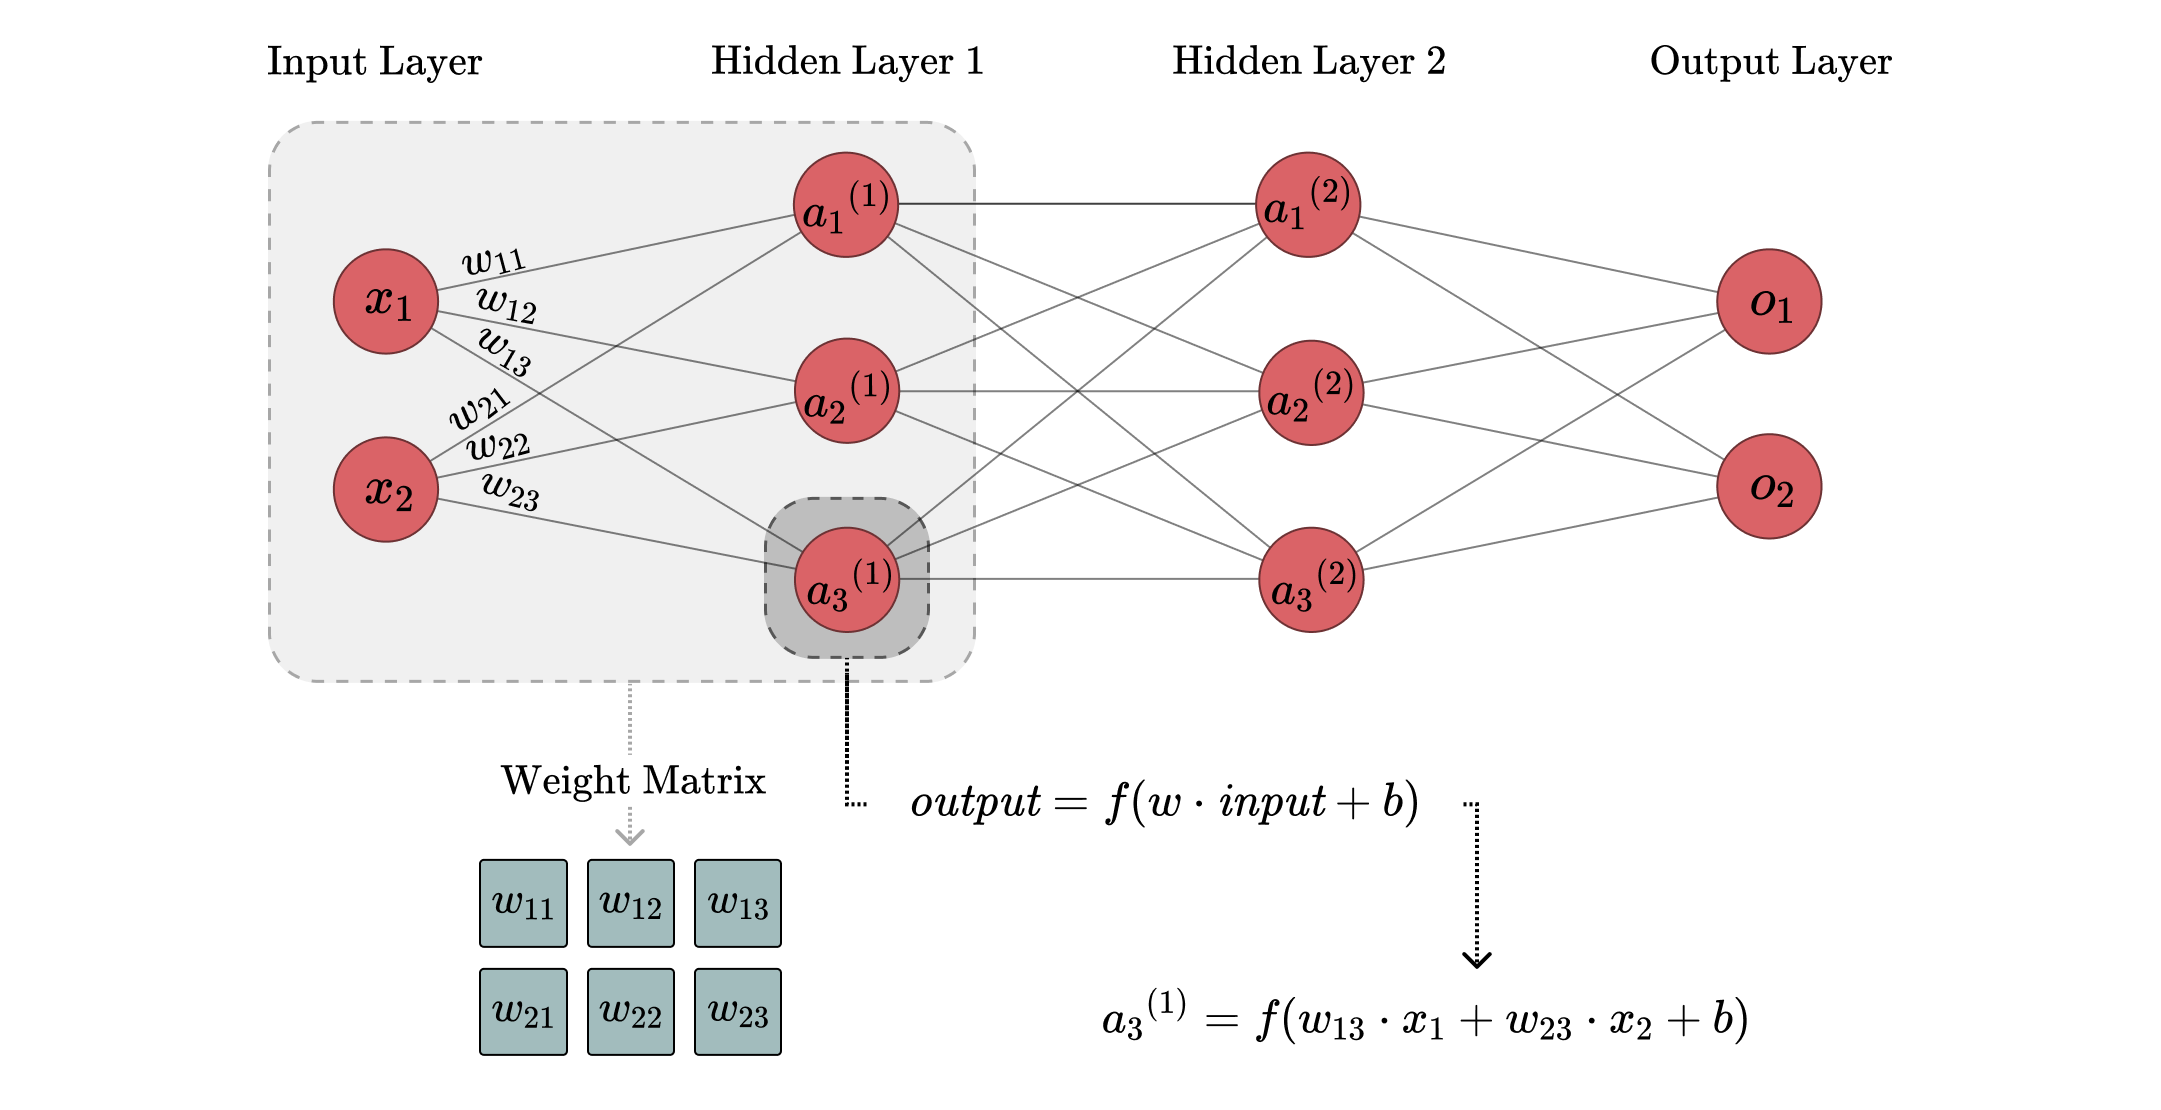
\includegraphics[width=14cm]{dense_layer}
  \caption{An example of a NN with two hidden dense layers, showing the connections between neurons in adjacent layers.}
  \label{fig:dense_layer}
\end{figure}

\noindent Mathematically, dense layers can be represented as:

\[
\textit{a} = f(W \cdot \textit{x} + b)
\]
\\
\noindent where:
\begin{itemize}
  \item \textit{x} is the input vector, representing outputs from the previous layer (or initial input data for the first layer).
  \item \textit{W} is the \textit{weight matrix}, with each row corresponding to the weight vector \( w \) of a specific neuron.
  \item \textit{b} represents the bias vector, where each scalar element corresponds to the bias of a specific neuron.
  \item \textit{f} is the \textit{activation function} that is applied element-wise.
  \item \textit{a} refers to the output vector, representing the activations of all neurons.
\end{itemize}

\noindent This interconnectedness of dense layers introduces the inherent redundancy, 
or the over-parameterizedness of NNs \cite{gholami2021survey}. It is particularly true in models with a large number of neurons, 
where \( W \) results in a vast number of parameters, which do not contribute to the model accuracy equally \cite{hubara2016qnn}.
\\
\\
\noindent \textit{Convolutional layers} are another type of hidden layers 
that involve a \textit{convolution} operation on the input. Intuitively, a standard convolution is 
a process of sliding a small grid over an input to find patterns. The figure below, for example, shows 
the application of the Sobel kernel that detects edges on the input image.

\begin{figure}[h!]
  \centering
  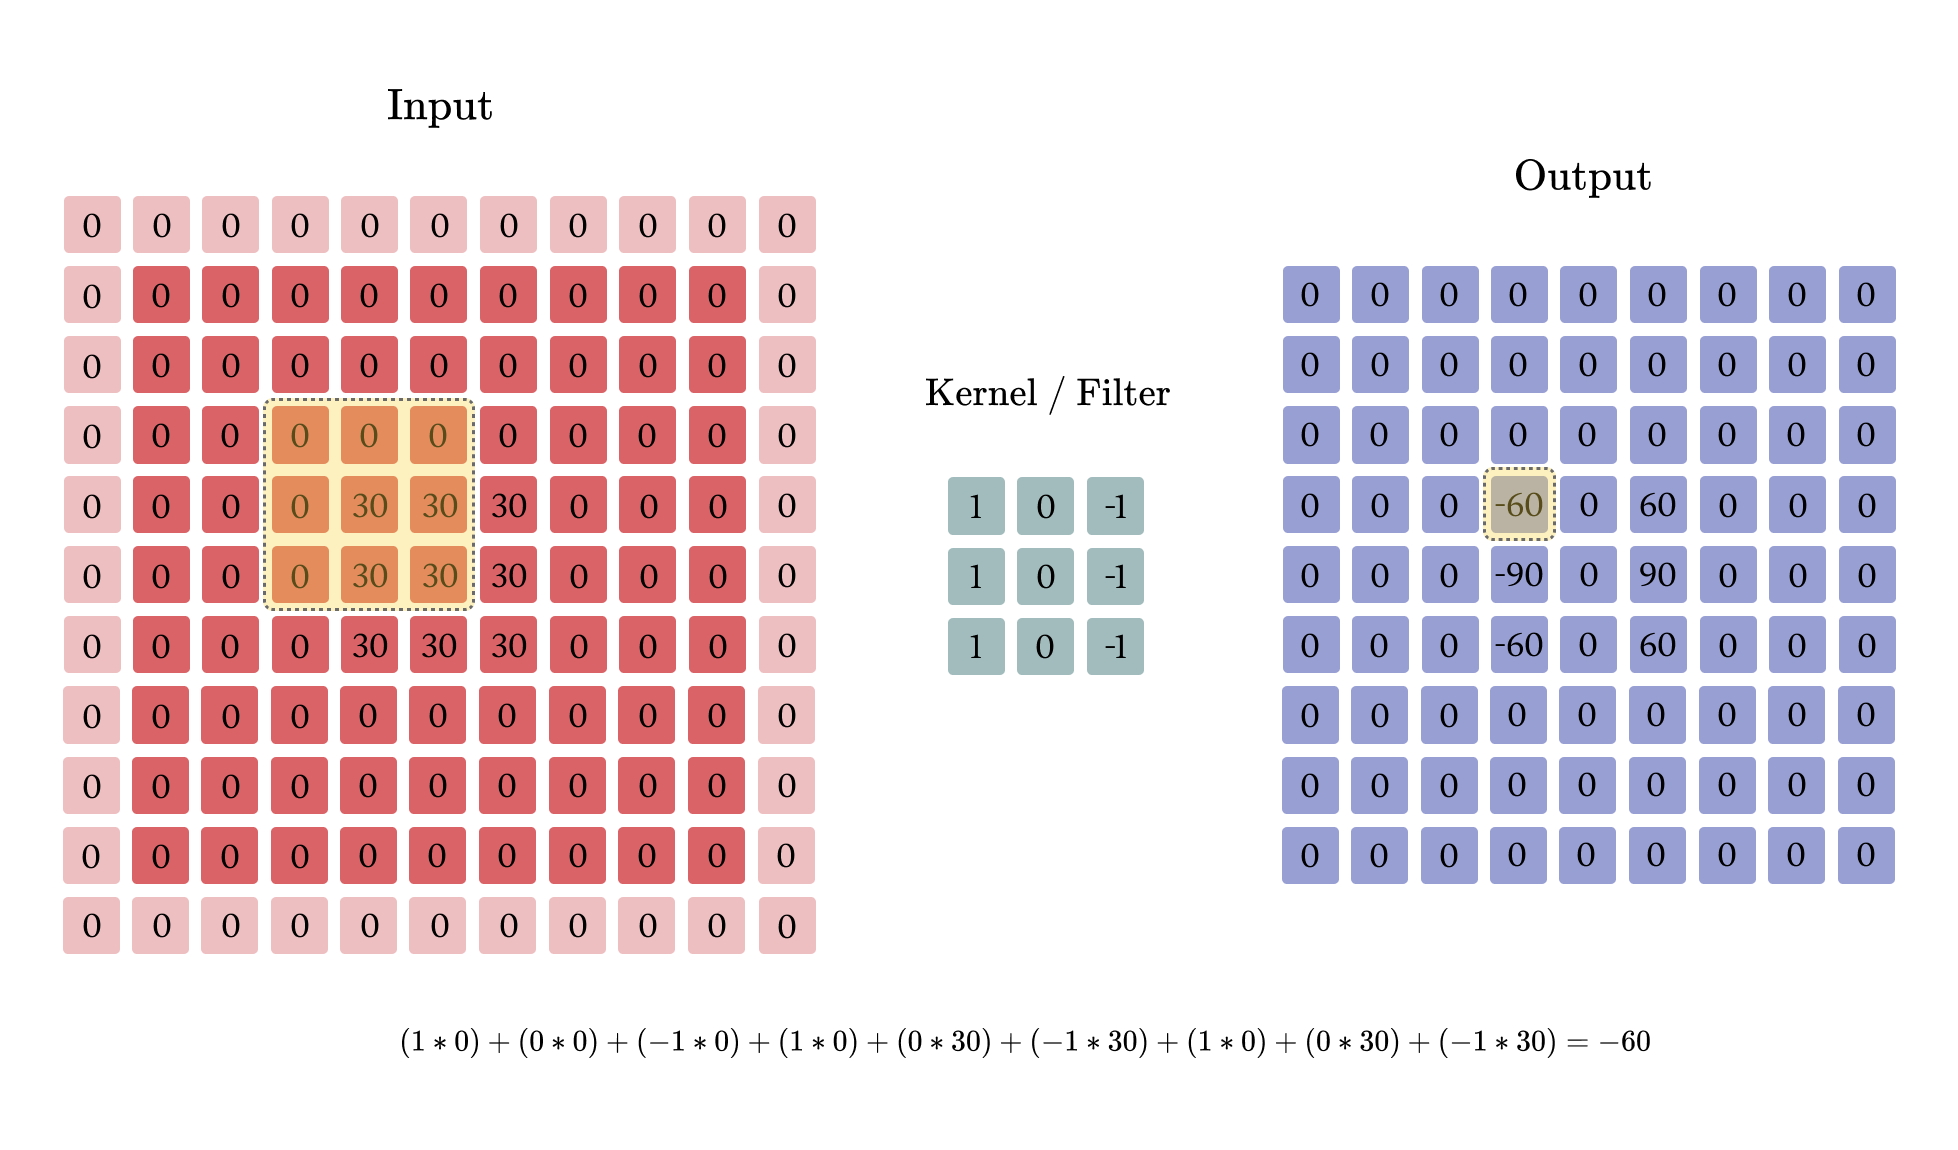
\includegraphics[width=14cm]{convolution}
  \caption{A 3×3 kernel (filter) sliding over a padded input matrix to compute the output feature map, demonstrating the interaction between the kernel weights and input values at a specific position.}
  \label{fig:convolution}
\end{figure}

\noindent For multi-channeled inputs, like RGB images, the convolution operation uses a multi-channeled kernel, as shown in Figure 2.3, 
producing a single-channeled feature map that combines weighted contributions from all input channels. 
A convolutional layer typically includes multiple such kernels, generating feature maps equal to the number of kernels.
After the convolution operation generates the feature maps, a bias term is added to each map, 
and the activation function is applied element-wise — just like in dense layers.

\begin{figure}[h!]
  \centering
  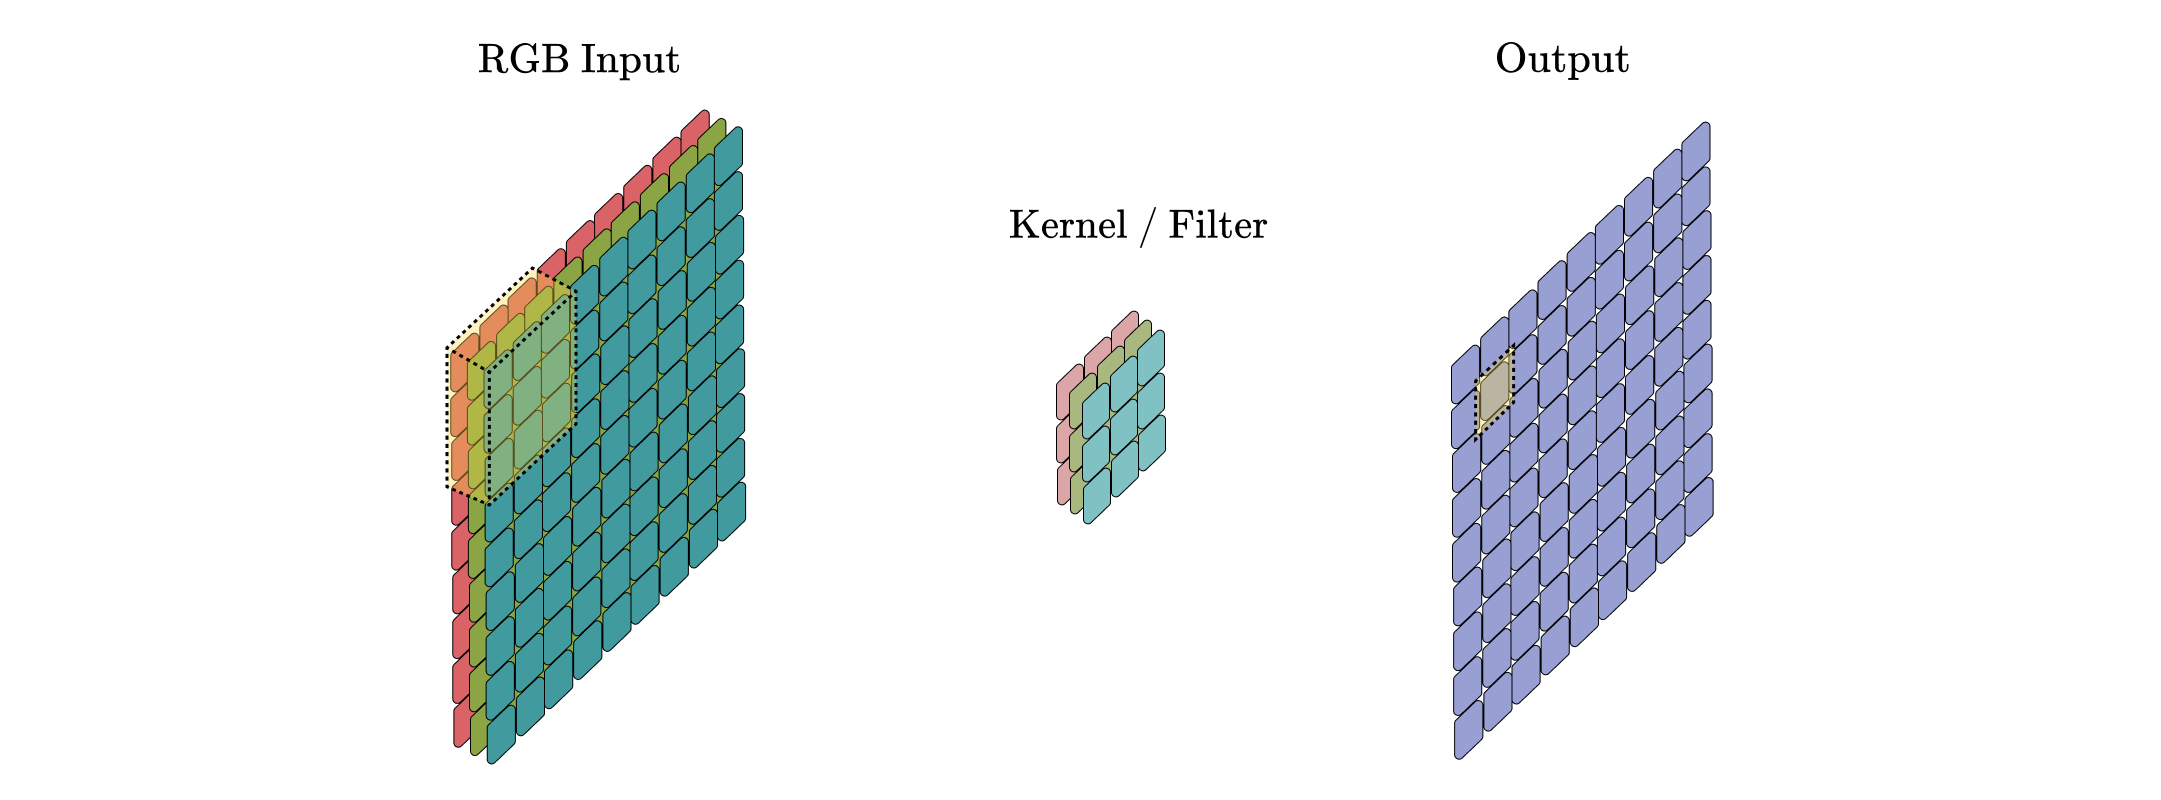
\includegraphics[width=14cm]{convolution_multiple_channels.png}
  \caption{A 3×3x3 kernel (filter) sliding over an RGB input matrix to produce a single-channeled output feature map.}
  \label{fig:convolution_multiple_channels}
\end{figure}

\noindent Mathematically, a convolutional layer can be represented as:

\[
y_{i,j,k} = \phi \left( \sum_{m=1}^M \sum_{p=1}^P \sum_{q=1}^Q x_{i+p-1, j+q-1, m} \cdot w_{p,q,m,k} + b_k \right)
\]
\\
\noindent where:
\begin{itemize}
  \item \( P, Q \) are the height and width of the filter, respectively.
  \item \( M \) is the number of input channels.
  \item \( y_{i,j,k} \) denotes the output at position \((i, j)\) for the \(k\)-th filter.
  \item \( x_{i+p-1, j+q-1, m} \) is the input at position \((i+p-1, j+q-1)\) for the \(m\)-th input channel.
  \item \( w_{p,q,m,k} \) represents the weight of the filter at position \((p, q)\) for the \(m\)-th input channel and \(k\)-th filter.
  \item \( b_k \) is the bias for the \(k\)-th filter.
  \item \( \phi(\cdot) \) is the activation function.
\end{itemize}

\noindent In simpler terms, a convolutional layer applies filter weights 
as it slides over rows \((p)\), columns \((q)\), and channels \((m)\), 
sums the results, adds bias \((b_k)\), 
and repeats this for all positions \((i, j)\) and filters \((k)\).
\\
\\
\noindent Although convolutional layers often have fewer weight parameters than dense layers in typical architectures, 
they still contain redundancies \cite{huang2017densely}, presenting an opportunity for quantization. 
Thus, both dense and convolutional layers will be the focus of this work.

% -------------------- lossregularization --------------------

\subsection{Loss Functions and Regularization}
\label{subsec:lossregularization}
The weights and biases are usually \textit{learnable parameters}
that the model adjusts during \textit{training}.
The training process of NNs is similar to how our brains learn from mistakes. 
Given the ground truth, a NN adjusts its learnable parameters 
using a specific function that compares the ground truth with the output generated by the network, 
essentially measuring the magnitude of the network's errors.
\\
\\
This function is called a \textit{loss function}, and depending on the type of question the network aims to answer, it can take many different forms.
For example, for the MLP described in Figure~\ref{fig:dense_layer} that generates a binary classification, we would use the \textit{log loss} function. 
Since the datasets used in this thesis involve multi-class classification, the \textit{sparse categorical cross-entropy} (SCCE) loss function will be used, 
which measures the difference between the predicted class probabilities and the true labels for each class in the dataset.
\\
\\
Often the loss function alone is not enough for a NN to perform well, 
as it may lead to overfitting or fail to capture desired generalization properties.
This is why a \textit{regularization term} that penalizes unwanted behaviours
is added to the loss function.
\\
\\
A typical regularization term is \( L_2 \), 
which penalizes large weights by adding the sum of the squared weights to the loss. 
The modified loss function is then expressed as:

\[
\mathcal{L}_{\text{total}} = \mathcal{L}_{\text{data}} + \lambda \sum_{i} w_i^2
\]
\\
\noindent where:

\begin{itemize}
  \item \( \mathcal{L}_{\text{data}} \) is the original loss function (in our case, the SCCE loss function).
  \item \( \lambda \) is a scalar parameter that controls the strength of the regularization.
  \item \( w_i \) represents each individual weight value in the model.
\end{itemize}

\noindent The current work employs multiple custom regularization terms 
that encourage specific behaviors in the models while discouraging others. 
These terms will be discussed in detail in the Experimental Setup section \ref{sec:setup}.

% -------------------- forwardback --------------------

\subsection{Forward-Pass and Back-Propagation}
\label{subsec:forwardback}
The repetition of the mathematical operations described earlier in the Dense and Convolutional Layers subsection \ref{subsec:denseconvolutional} 
during model training constitutes the \textit{forward pass}. 
It is the process where input data is passed through the network layer by layer, 
with each layer applying its learned weights and biases to produce a final output. 
\\
\\
As mentioned in the previous subsection, this output is then compared with the ground truth by the loss function that produces an error.
This error is used to update the learnable parameters in \textit{W} and \textit{b} during a process called \textit{back-propagation}.
\\
\\
In other words, back-propagation is the method by which the network adjusts its parameters to minimize the error. 
It calculates the gradient of the loss function with respect to each parameter using the chain rule. 
\( W \) and \( b \) are typically updated as follows:

\[
W = W - \eta \frac{\partial L}{\partial W}, \quad b = b - \eta \frac{\partial L}{\partial b}
\]
\\
\noindent where \( L \) is the loss function, and \( \eta \) is the learning rate.
\\
\\
For example, consider the weight \( w_{1,1} \) represented as the line between \( x_1 \)
 and the hidden layer node \( {a_1}^{(1)} \) in Figure~\ref{fig:dense_layer}. 
The gradient of this weight with respect to the loss is calculated using the chain rule:

\[
\frac{\partial L}{\partial w_{1,1}} = \frac{\partial L}{\partial o_1} \cdot \frac{\partial o_1}{\partial {a_1}^{(1)}} \cdot \frac{\partial {a_1}^{(1)}}{\partial w_{1,1}}
\]

\noindent Where:
\begin{itemize}
    \item \( \frac{\partial L}{\partial o_1} \) is the gradient of the loss with respect to \( o_1 \).
    \item \( \frac{\partial o_1}{\partial {a_1}^{(1)}} \) is the gradient of \( o_1 \) with respect to the output of \( {a_1}^{(1)} \).
    \item \( \frac{\partial {a_1}^{(1)} }{\partial w_{1,1}} \) is the value of  \( x_1 \), since  \( {a_1}^{(1)} \) is a weighted sum of the inputs.
\end{itemize}

\noindent This shows how each weight contributes to the final error during back-propagation.

% ------------------------------------------------------------
% ----------------------- basicsofquantization ----------------------- 
% ------------------------------------------------------------

\section{Basics of Quantization}
\label{sec:basicsofquantization}
This section aims to answer the \textit{why} question with respect to quantization and further provides a broader understanding of the term regarding its types.

% -------------------- purpose and definition --------------------

\subsection{Purpose and Definition}
\label{subsec:purposeanddefinition}
As we become increasingly dependent on deep learning models disguised as everyday tools, 
the need for these models to function in a resource- and time-efficient manner is more imperative than ever. 
The focus on resource efficiency is particularly important, 
with the research community expressing concerns regarding the environmental effects of large models, 
the exponential size growth of which continues to significantly outpace that of system hardware \cite{DBLP:journals/corr/abs-2111-00364}. 
In this regard, studies have examined quantization within the context of Green AI as a method to reduce the carbon footprint of
ML models \cite{DBLP:journals/csi/RegueroMV25}.
\\
\\
Aside from the environmental considerations, the mere need to reduce 
the computational cost and speed of predictive models
comes as an apparent business requirement. 
This requirement is essential when — quite ironically — embedded systems, famous for their compactness, meet 
ML models, infamous for their complexity. Microcontrollers, for instance, 
usually are not able to perform floating-point operations, which must therefore be emulated in software, 
introducing significant overhead. This is why quantization, the process which reduces the memory footprint of a model,
is also extensively covered in the realm of embedded systems that 
inherently prefer integer arithmetic \cite{DBLP:conf/codit/KhalifaM24}\cite{DBLP:journals/corr/abs-2105-13331}.
\\
\\
Another motivation for quantization — although somewhat controversial — is the fact that reducing the bit-width of
ML models makes them robust to adversial attacks in certain cases \cite{DBLP:journals/corr/abs-2404-05639}.
This holds significant value in fields, such as autonomous driving,
where model vulnerability may result in fatal outcomes.
Interestingly enough, the use cases where such robustness is required also demand fast inference, 
as they rely on real-time predictions. Consider healthcare diagnostics needed for emergency scenarios 
or military defense mechanisms designed for immediate action.
\\
\\
The list of reasons why quantization is useful may go on for a while, but regardless of the motivation,
the essence of the term itself — rooted in the early 20th century — remains unchanged:
quantization refers to the division of a quantity into a discrete number
of small parts \cite{gray1998quantization}. With regard to ML models, 
it describes the process of dividing higher bit-width numbers into a discrete number of lower bit-width representations
without causing significant degradation in performance \cite{gholami2021survey}.
\\
\\
Since ML models are generally considered redundant or over-parameterized,
there are multiple points where quantization can be applied.
Specifically, in this thesis, we apply quantization to the weights and biases of dense layers, 
as well as the kernels and biases of convolutional layers. 
Although not explicitly a part of a model, we also explore input data quantization. 
Other applications include, but are not limited to, layer activation and layer input quantization (two sides of the same coin),
as well as gradient quantization. The bottom line is that wherever there is an opportunity for arithmetic or memory optimization,
there is room for quantization.

% -------------------- Common Quantization Approaches --------------------

\subsection{Core Quantization Approaches}
\label{subsec:commonquantizationapproaches}

There is a multitude of ways to classify NN quantization methods, a broader overview of which will be covered
in the Related Work chapter \ref{cha:chapter5}.
For now, we will focus on a few basic approaches from the general categories of both 
\textit{data-driven} and \textit{data-free} methods \cite{Edouard2022SPIQ} to provide a basic understanding of the NN quantization process.
\\
\\
The simplest form of data-free quantization, or \textit{post-training quantization} \cite{jiang2021efficient},
involves converting already trained parameters from FP32 to a lower bit-width format
without using the initial training data. 
A common approach is to apply \textit{uniform quantization} that maps real values to a set number
of \textit{bins}. The general formula can be written as:

\[
Q(r) = round(\frac{r}{S})
\]

\noindent Where:
\begin{itemize}
    \item $Q(\cdot)$ denotes the quantization operation.
    \item $r$ is the real value of a given model parameter in higher bit-width representation.
    \item $round(\cdot)$ is some rounding operation, such as a simple $floor(\cdot)$.
    \item $S$ is a scaling factor.
\end{itemize}

\noindent  As a result, we essentially end up with a discrete number of values in lower bit precision, 
instead of an almost continuous range of real numbers as shown in Figure \ref{fig:quantizing_example}.
\\
\begin{figure}[h!]
  \centering
  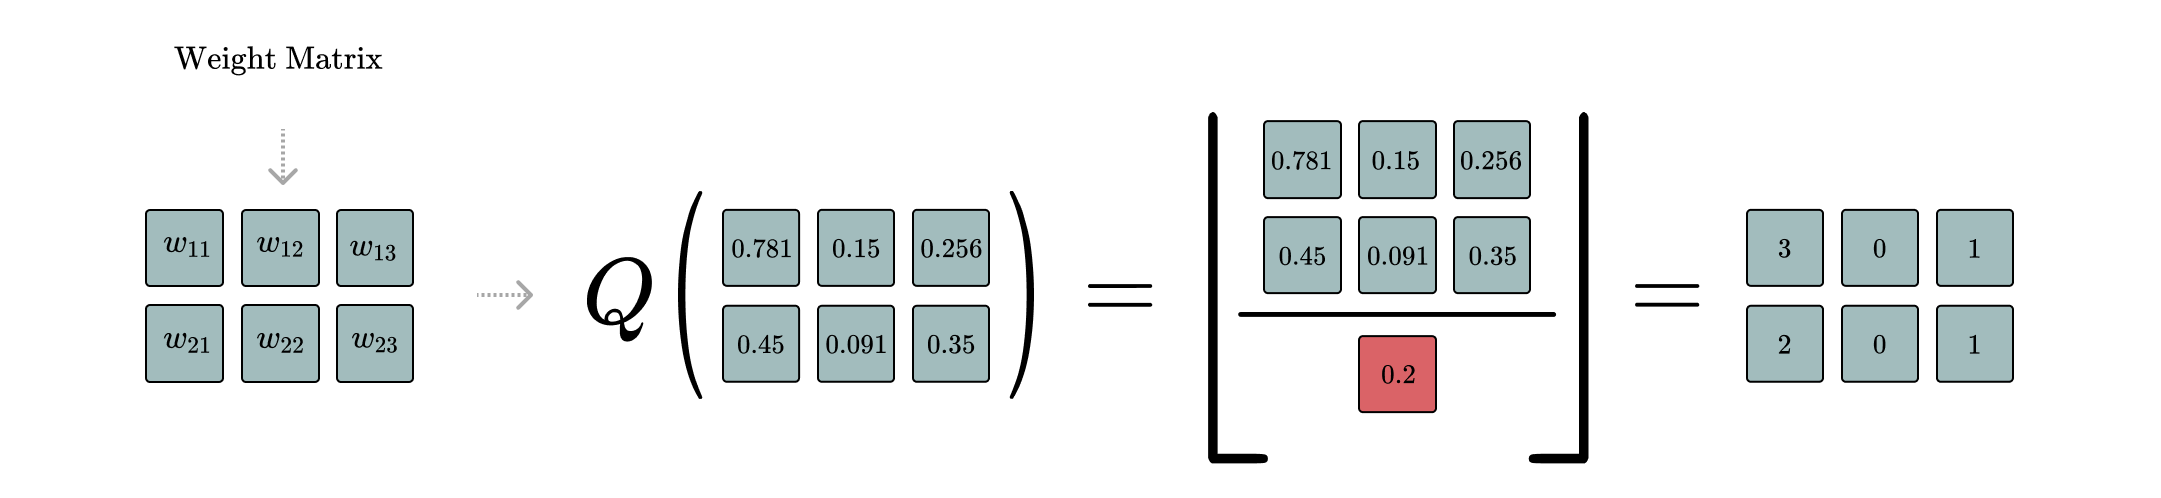
\includegraphics[width=10cm]{quantizing_example.png}
  \caption{An example illustrating the quantization operation on the weight matrix from Figure \ref{fig:dense_layer}, 
  with arbitrary values for demonstration purposes.}
  \label{fig:quantizing_example}
\end{figure}

\noindent Unlike data-free quantization  —  as the name suggests — data-driven quantization typically involves retraining the model
using the initial data. An example of this approach is the Ristretto framework \cite{DBLP:journals/tnn/GyselPMG18}, which, similar to data-free methods, 
first analyzes the trained model to select suitable lower bit-width number formats for its weights.
Then, using a portion of the original dataset, the framework determines appropriate formats for layer inputs and outputs.
As a next step, based on the validation data, Ristretto adjusts the quantization settings to achieve optimal performance 
under the given constraints. Finally, the quantized model is fine-tuned using the training data.
\\
\\
A much simpler example of data-driven quantization could be the min-max quantization on input data as shown in Figure \ref{fig:min_max_quantization}. 
This method can also be used in a data-free scenario to quantize learned model parameters and is internally used as one of the
default techniques in popular ML frameworks like Tensorflow and PyTorch.

\begin{figure}[h!]
  \centering
  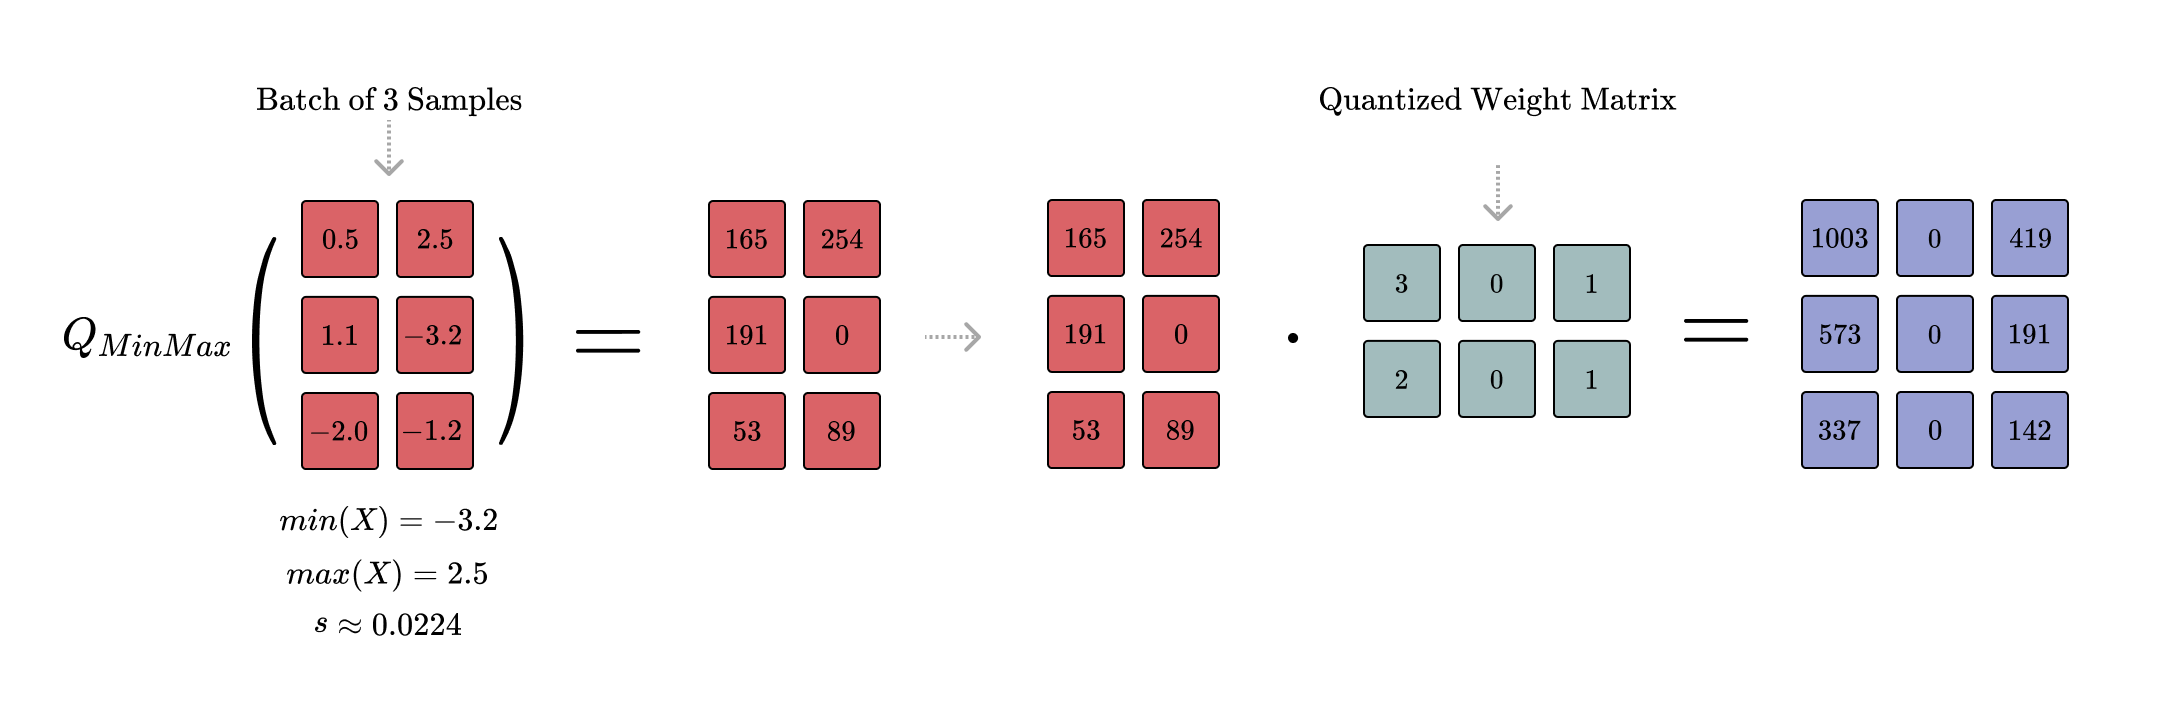
\includegraphics[width=15cm]{min_max_quantization.png}
  \caption{ An example illustrating min-max quantization of input data to 8 bits, followed by matrix multiplication with the quantized weight matrix from Figure \ref{fig:quantizing_example}.
  Input data has arbitrary values for demonstration purposes.}
  \label{fig:min_max_quantization}
\end{figure}

\noindent In the previous subsection, we discussed \textit{where} quantization could be applied in a model, 
mentioning weights, kernels, and biases as the focus of this thesis.
Figures \ref{fig:quantizing_example} and \ref{fig:min_max_quantization} show examples of quantization
using a scalar scaling factor. However, scaling factors could be applied at varying levels of detail,
and this is where the concept of \textit{quantization granularity} comes into play.
\\
\\
Granularity refers to the level of detail at which scaling factors are applied,
ranging from a single factor for an entire kernel (coarse granularity) to separate factors for individual spatial locations,
channels, or filters (fine granularity). For instance, Figure \ref{fig:granularity-conv2d} illustrates various possible granularities
for the kernels of convolutional layers.
Despite this wide range of possibilities, channel-wise quantization is currently the standard for convolutional layers \cite{gholami2021survey},
as it helps parallel processing capabilities of accelerators that compute channel outputs independently. 
For dense layers, row-wise quantization (one scaling factor for weights used by a single output neuron) is more prevalent
because it aligns with matrix-vector multiplication, which then can be carried out by specialized linear algebra libraries
in an optimized way \cite{DBLP:journals/corr/abs-2101-05615}.

\begin{figure}[h!]
  \centering
  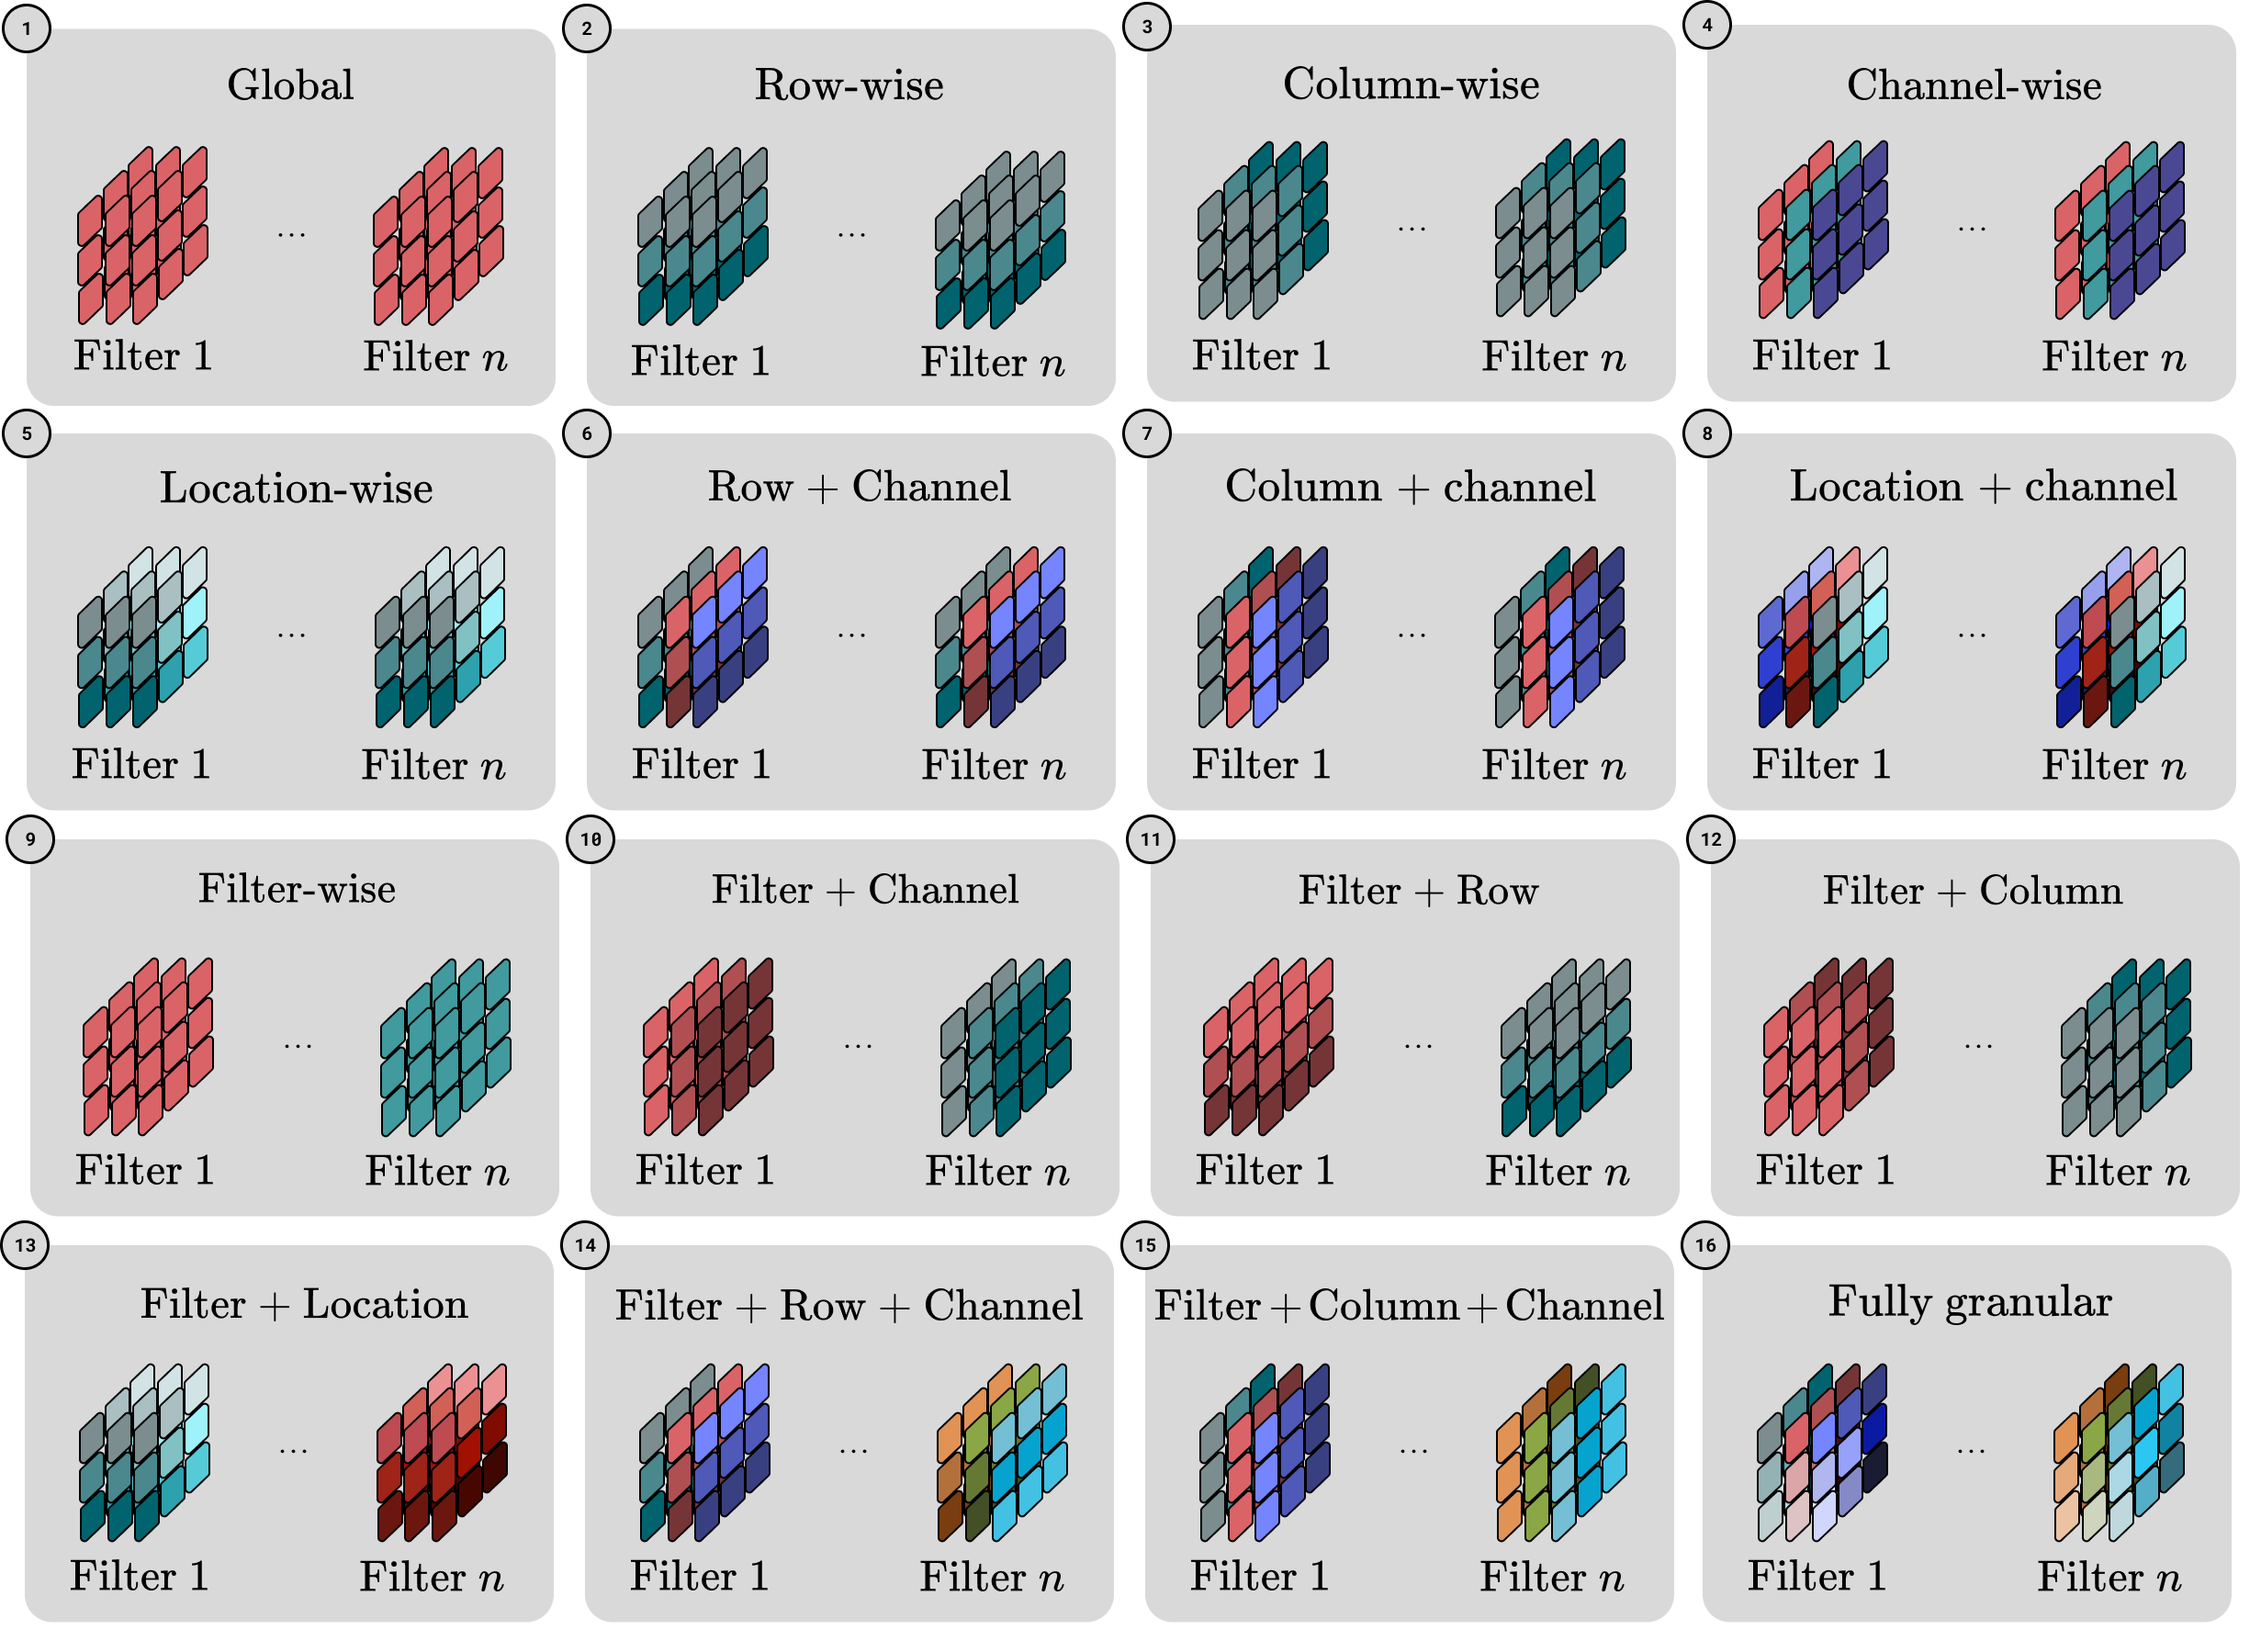
\includegraphics[width=15cm]{granularity-conv2d.png}
  \caption{A demonstration of the varying application of scaling factors, ranging from a single scalar applied to the entire kernel (1) to separate scalars assigned to spatial dimensions (e.g., 1, 2), channels (4), filters (9), and other granular configurations.}
  \label{fig:granularity-conv2d}
\end{figure}



% ------------------------------------------------------------
% ----------------------- learnedquantization ----------------------- 
% ------------------------------------------------------------
\section{Learned Quantization}
\label{sec:section3}
Now that the fundamentals of quantization have been covered, 
this section introduces key concepts commonly encountered in learned quantization,
including its challenges, trade-offs, and the popular techniques used to overcome them.


% -------------------- tradeoffs and challenges --------------------

\subsection{Trade-offs and Challenges}
\label{subsec:subsection1}
The inherent — or rather the generally accepted — characteristic of quantization is
that it negatively influences performance. 
This is referred to as the trade-off between quantization and generalization, 
which reflects the question of how much accuracy — or whatever performance metric is being used — 
we are willing to sacrifice to gain a reduction in computational cost, memory usage, or inference time.
However, the truth is that we usually cannot afford sacrificing anything.  This, coupled with the lack of a guarantee
 that pre-defined \textit{quantizers} can yield optimal results \cite{DBLP:conf/eccv/ZhangYYH18} \cite{DBLP:conf/iclr/EsserMBAM20}, 
 has paved the way for the burgeoning field of learned quantization,
 which aims to \textit{learn} how to quantize the model in a manner that mitigates performance loss.
\\
\\
Learned quantization is, however, a double-edged sword in the sense that, despite producing compact results,
the cost to achieve them is higher \cite{DBLP:conf/eccv/ParkYV18}. The obvious reason is the additional computational overhead
introduced by learnable quantizers.
Thus, it is important to strike a balance between learning optimal quantization and keeping the training process manageable
— which explains the prevailing emphasis on simplicity in most learned quantization research.
\\
\\
The main issue in achieving this simplicity is posed by the fact that discretization, in its essence, is non-differentiable
 — meaning it is challenging to integrate any kind of discretizing operations into gradient-based optimization methods, 
 upon which ML models rely. Using the chain rule back-propagation example from subsection \ref{subsec:forwardback}, let's
consider a simple flooring operation introduced into the process to better understand the problem.
\\
\\
Suppose we want to quantize activations and apply \( floor(\cdot) \) to hidden layer outputs:
\[
  {a_{1,q}}^{(1)} =  floor({a_1}^{(1)})
  \]
As a result, the chain rule becomes:
 \[
  \frac{\partial L}{\partial w_{1,1}} =  \frac{\partial L}{\partial {a_{1,q}}^{(1)}} 
  \cdot \frac{\partial {a_{1,q}}^{(1)}}{\partial {a_1}^{(1)}} 
  \cdot \frac{\partial {a_1}^{(1)}}{\partial w_{1,1}}
  \]
  
  \noindent where \( \frac{\partial {a_{1,q}}^{(1)}}{\partial {a_1}^{(1)}} \) presents a challenge. 
  Since \(  {a_{1,q}}^{(1)} =  floor({a_1}^{(1)}) \), the derivative is: 
            \[
            \frac{\partial a_{1,q}^{(1)}}{\partial a_{1}^{(1)}} =
            \begin{cases} 
                0 & \text{if } a_{1}^{(1)} \notin \mathbb{Z}, \\
                \text{undefined} & \text{if } a_{1}^{(1)} \in \mathbb{Z}.
            \end{cases}
            \]
  This means that for most values of \( {a_1}^{(1)} \), which are non-integer, the gradient becomes $0$, resulting in 
  $w_{1,1}$ not receiving any updates. For integer values of \( {a_1}^{(1)} \), the backpropagation process fails altogether.
\\
\\
In essence, circumventing the issue of non-differentiability is the fundamental problem that learned quantization aims to solve,
all while managing the aforementioned trade-offs to produce a model that is compact, not overly complex to train,
and highly performant.

\subsection{Common Methods}
\label{subsec:subsection2}
STE
\begin{itemize}

  \item In \textbf{learned quantization}, quantization parameters are learned as part of the model training process.
  This corresponds to Quantization Aware Training (QAT) \cite{jacob2018quantization}, where quantization is integrated directly into training rather than applied afterwards.
  Since learned quantization is central to this work, a detailed review of QAT and its applications is provided in the Related Work chapter. 

\end{itemize}

learned parameter



%\subsection{Low-Precision Forward-Pass}
%\label{subsec:subsection1}
%In QAT, the operation performed during the forward-pass is often modified. Instead of propagating the full precision values, 
%the output of a layer is first quantized and then dequantized before being passed to the next layer \cite{jacob2018quantization}. 
%This simulates the effect of quantization during inference, helping the network adjust to the reduced precision parameters.
%\\
%\\
%The \textit{quantization} process can be generalized as follows:
%
%\[
%q(x) = \text{round}\left( \frac{x}{P} \right) - Z
%\]
%\\
%\noindent where \( q(x) \) is the quantized value, \( x \) is the full precision value of the parameter that is being quantized, \( P \) is a quantization parameter, such as a scaling factor, 
%and \( Z \) represents the zero point. This method is the most commonly used \textit{uniform quantization}, which can be either \textit{asymmetric} or \textit{symmetric}, 
%depending on the value of \( Z \), with  \( Z \) = 0 representing \textit{symmetric quantization}.
%\\
%\\
%For \textit{dequantization}, we apply:
%
%\[
%x_{\text{dequant}} = P \cdot ( q(x) + Z)
%\]
%\\
%\noindent Note that the dequantized value does not necessarily match the initial value. 
%For example, if \( x = 7.8 \) and \( P = 2 \), then quantization gives \( q(x) = 4 \), and dequantization results in \( x_{\text{dequant}} = 8 \). 
%This demonstrates how the \textit{quantization} and dequantization process approximates the original value \( x \)
%by rounding it to the nearest representable value based on the quantization parameter \( P \).

%\subsection{Full-Precision Back-Propagation}
%\label{subsec:subsection1}
%In QAT, although the forward-pass operates on quantized values, back-propagation typically uses full-precision values. 
%This is because the rounding operation in the forward-pass is non-differentiable, which makes it impossible to compute gradients directly \cite{polino2018modelcompression}.
%\\
%\\
%Consider the example of computing the gradient of the weight \( W_{I1,H1_1} \) in Figure~\ref{fig:mlp_diagram}:
%
%\[
%\frac{\partial L}{\partial W_{I1,H1_1}} = \frac{\partial L}{\partial \text{Output 1}} \cdot \frac{\partial \text{Output 1}}{\partial H1_1} \cdot \frac{\partial H1_1}{\partial W_{I1,H1_1}}
%\]
%\\
%\noindent If the output of \( H1_1 \) was quantized using a rounding operation, the gradient 
%\[
%\frac{\partial H1_1}{\partial W_{I1,H1_1}} 
%\]
%would be undefined due to the non-differentiability of rounding. This would break the gradient flow, making it impossible to update  \( W_{I1,H1_1} \)
%during back-propagation.
%\\
%\\
%To work around this, techniques such as the Straight-Through Estimator (STE) are commonly used \cite{bengio2013estimating} \cite{fan2021training} \cite{zhuang2018towards} \cite{krishnamoorthi2018quantizing}.
%The STE approximates the gradient by treating the rounding function as if it were differentiable during the back-propagation.
%This approach ensures that the model can simulate low-precision inference during the forward pass,
%while still benefiting from the accuracy of full-precision gradient updates during back-propagation.
%\\
%\\
%The Experimental Setup section will explain a slighly different version of the typical STE that was used in the current work.

THIS PART WILL GO TO THE NEXT SECTION:
\\
\\
An example approach is to define a regularization term that directly penalizes large differences between full-precision values 
and their quantized counterparts \cite{zhuang2018towards}. This can encourage the model to learn parameters that are easily quantizable without significant performance loss.
If the values that are being quantized are \( W \), then this regularization term could look like:

\[
\mathcal{L}_{\text{quant}} = \lambda \sum_{i} \| W_i - q(W_i) \|^2
\]

\noindent Where:
\begin{itemize}
    \item \( \lambda \) is a scalar that controls the importance of the quantization penalty.
    \item \( W_i \) represents the full-precision weight value before quantization at index \( i \).
    \item \( q(W_i) \) represents the quantized version of \( W_i \).
\end{itemize}

\noindent The current work uses multiple custom regularization terms that trigger the quantization process during training. 
These will be discussed in detail in the Experimental Setup section.

    \chapter{Learned Quantization\label{cha:chapter3} Schemes}
This chapter introduces two custom learned quantization schemes — approaches that allow models to learn to quantize themselves
with adjustable aggressiveness. The first one, a custom quantization layer featuring a threshold for gradient based scale updates,
will be discussed in the first section. The second scheme, which focuses on custom regularization terms with a configurable penalty rate,
will be covered second.

% ------------------------------------------------------------
% ----------------------- learnedquantization Schemes ----------------------- 
% ------------------------------------------------------------

\section{Nested Quantization Layer}
\label{sec:nestedquantizationlayer}
To separate the quantization logic from the usual structure of NN layers,
we define a nested quantization layer that can be used within a standard one. 
This approach provides usability, making it easy to extend the functionality to other types of layers beyond dense and convolutional ones.
We will first explain the core logic of the nested quantization layer and how it integrates into a model,
followed by a detailed explanation of how the trainable scaling factors are updated.


% -------------------- Implementation details --------------------

\subsection{Core Logic and Structure}
\label{subsec:quantizedconvolutional}

As the name "nested quantization layer" suggests —
this layer is implemented in a way that it is initialized from within a model layer itself.
\\
\\
To explain, let \( P \) be the parameter of a layer (weights, bias or kernel). This \( P \) is used
as the input for the nested quantization layer, where it undergoes quantization based on 
a scaling factor \( s \). In turn, \( s \) is the only trainable parameter of the nested layer itself.
\\
\\
The forward pass of the nested layer performs the following operation:

\[
  P_{reconstructed} = P_{quantized} \cdot s
\]

\noindent where \( P_{quantized} \) is the quantized integer form of \( P \) and is defined as:

\[
  P_{quantized} = floor(\frac{P}{s})
\]

\noindent During backpropagation, the nested layer receives the upstream gradient of
\( P_{reconstructed} \) and passes it downward as is.  This follows the standard STE behaviour
used with non-differentiable discretizers, such as \( floor(\cdot) \) in our case,
as discussed in Subsection \ref{subsec:commonquantizationapproaches}.
\\
\\
For updating the scale factor \( s \) — its own trainable parameter — 
the nested layer utilizes the upstream gradient information of \( P_{\text{reconstructed}} \)
and applies a custom logic, which will be detailed in the next subsection. 
Essentially, this approach solves two problems with one tool — updating both 
\( P \) and \( s \) using the same gradient, although with different logic.
\\
\\
Conceptually, the resulting structure with one or more nested quantization layers is illustrated in Figure \ref{fig:nested_quantization}
on the example of a convolutional layer.
\\
\begin{figure}[h!]
  \centering
  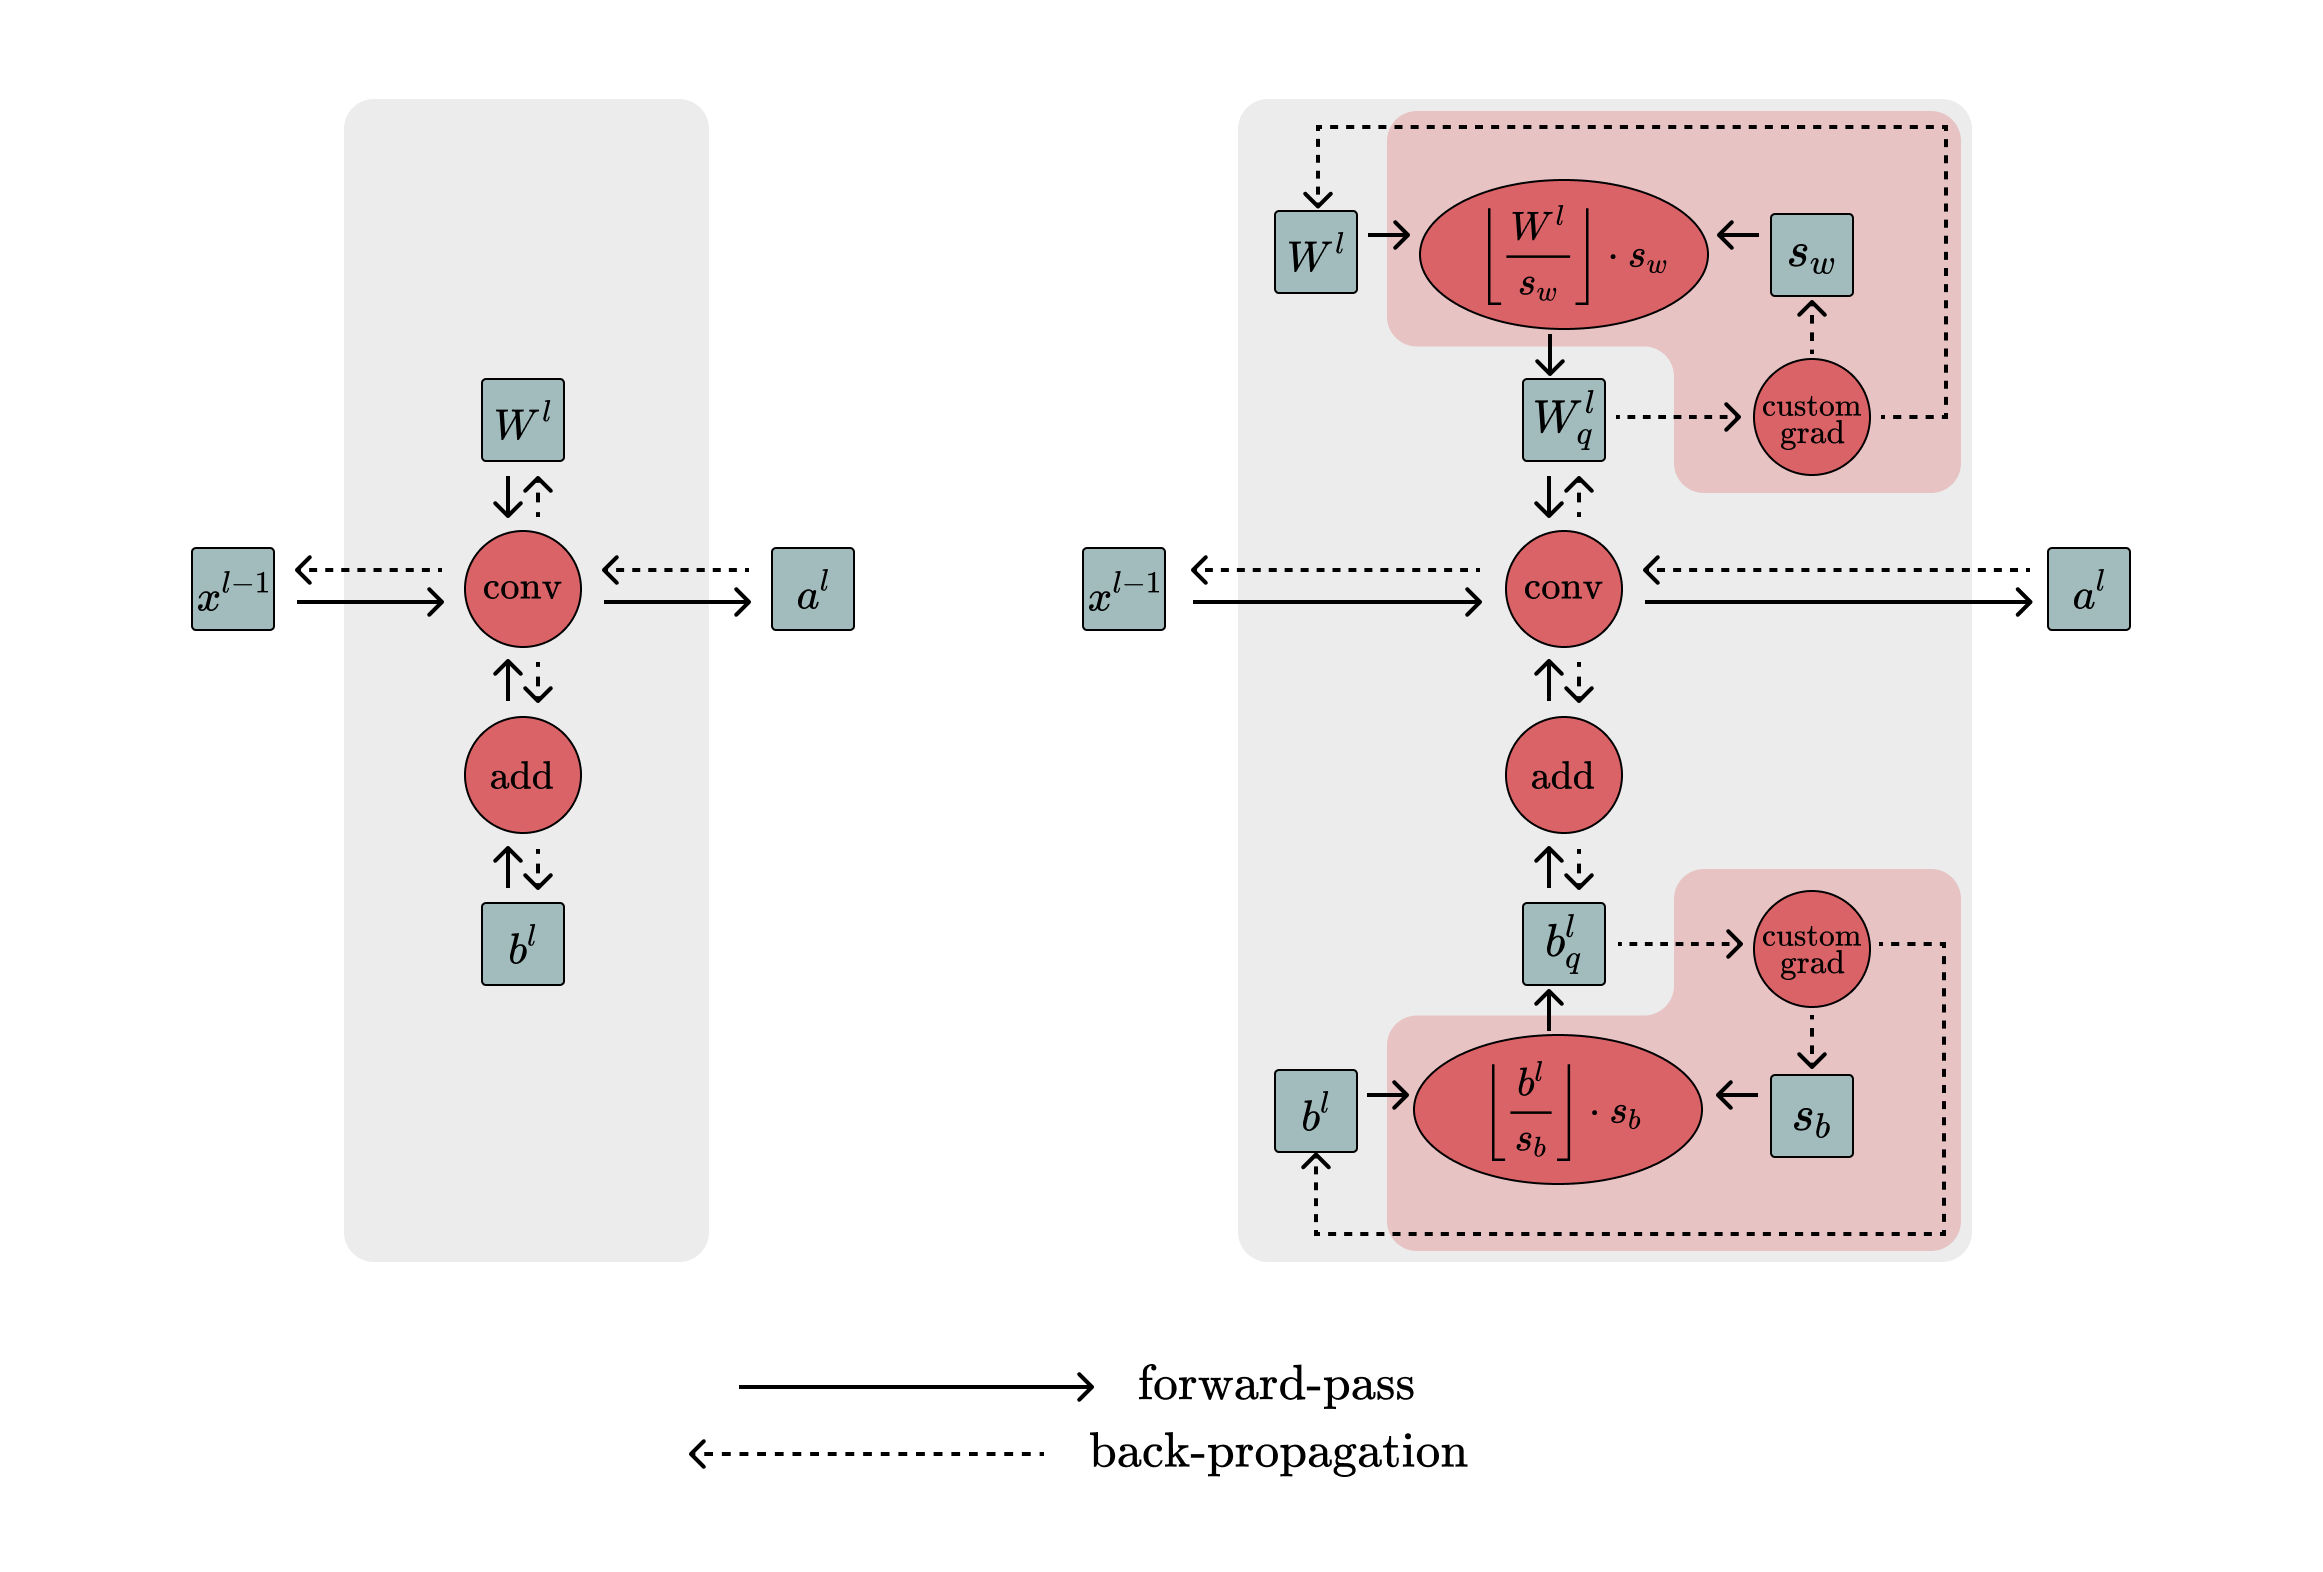
\includegraphics[width=14cm]{nested_quantization_layer.png}
  \caption{A standard convolutional layer (left) and its integration with the nested quantization layer (right) for both weights and bias.
  Quantization logic is applied to weights and biases during the forward pass, with trainable scaling factors 
  updated using custom gradients in the backward pass. Parameter gradients are passed downward as is.}
  \label{fig:nested_quantization}
\end{figure}

\noindent Since the scaling factor \( s \) can have different shapes and be applied at varying levels of granularity,
we have enabled scalar, row-wise, and column-wise application granularity for dense layers,
as shown in Figure \ref{fig:scaler-application-dense}. 
For convolutional layers, we additionally support channel-wise granularity,
corresponding to the first four scenarios in Figure \ref{fig:granularity-conv2d}.
\\
\begin{figure}[h!]
  \centering
  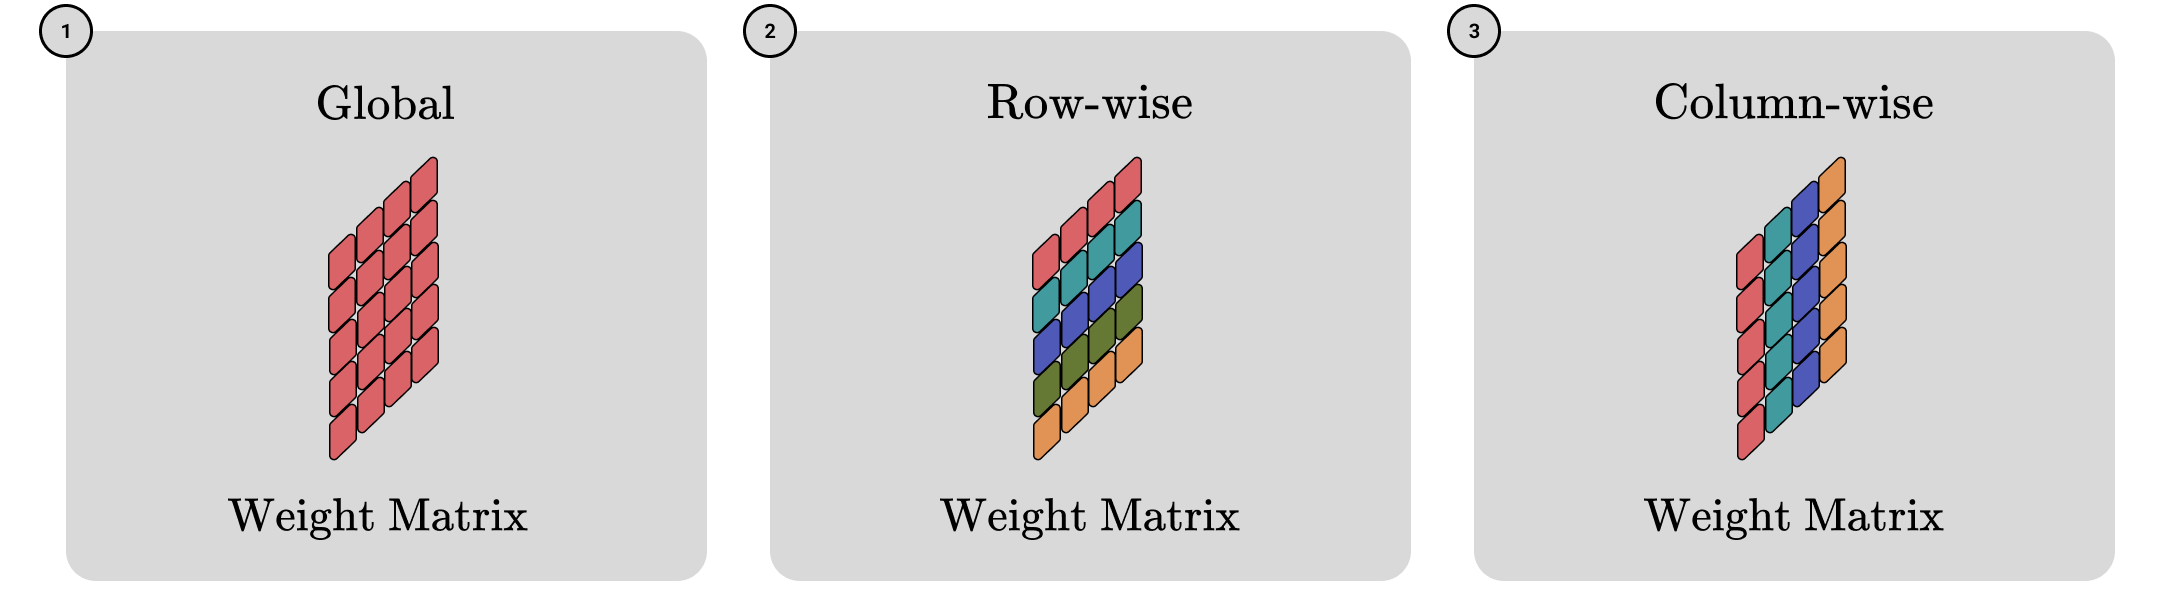
\includegraphics[width=14cm]{Scaler-application-dense.png}
  \caption{A demonstration of the varying applications of scaling factors, ranging from a single scalar applied to the entire weight matrix (1) to row-wise and column-wise application of vector scalers.}
  \label{fig:scaler-application-dense}
\end{figure}

\noindent The nested layer is built upon Tensorflow's \texttt{tf.keras.Layer} class,
which serves as the base for all Keras layers. The gradient calculation logic is wrapped
in Tensorflow's \texttt{tf.custom\_gradient} decorator, allowing proper functioning of the 
model's computational graph. Dense and convolutional layers have been implemented as 
\texttt{tf.keras.Layer} objects with minimal adjustments as well to incorporate the nested layers logic.

% -------------------- concept and design --------------------

\subsection{Learned Scale Factor}
\label{subsec:learnedscalefactor}

For the trainable scale factor \( s \), we define a custom gradient formula. 
The gradient of the loss with respect to \( s \), denoted as \( \nabla_s L \), is computed as:
\[
\nabla_s L = g_s \cdot m,
\]
Let's consider both multiplication terms separately. \(  g_s  \) is the main "decision maker" on whether to
increase the scale and, therefore, quantize more. It is based on a hyperparameter threshold  \(  \lambda  \),
which is compared against the ratio \(  r  \).

\[
g_s = 
\begin{cases} 
0, & \text{if } r \geq \lambda, \\
- \tanh(\lambda - r), & \text{if } r < \lambda,
\end{cases}
\]

\noindent In turn, \(  r  \) is the ratio between the upstream gradient of the layer's reconstructed parameter with respect to the loss
and its absolute value (for simplicity, we done \( P_{reconstructed}\) as \(P_r\)):

\[
r = \frac{\left| \nabla_{P_{r}} L \right|}{\max(\epsilon, \left| P_r \right|)}
\]

\noindent In essence, it conveys the relative impact of the gradient on the parameter's value.
A large ratio indicates that the parameter is not ready for aggressive quantization
because small perturbations can lead to significant changes in its optimization.
Conversely, parameters with a small \(  r  \) are better candidates
for quantization since they are less sensitive.
\\
\\
The decision to replace \( P_r \) with \( \epsilon \) when \( P_r = 0 \)
ensures that the corresponding \( r \) becomes large,
effectively resisting quantization. This behavior is valid regardless of the parameter's sensitivity
 — if the zero parameter is sensitive, quantization could disrupt future optimization steps,
 and if it is not sensitive, quantization adds no value since \( s \) has a positive non-zero constraint 
 and \( \frac{P}{s} \) will remain zero.
\\
\\
The motivation behind using \( tanh(\cdot) \) primarily stems from two key reasons. 
First, it is bounded (in our use case, to \( [-1, 0) \)), which prevents excessive gradient magnitudes.
Second, unlike sigmoid, it does not require any additional rescaling since it is
symmetric around \( 0 \). An additional point is that \( tanh(\cdot) \) saturates comparably faster,
potentially allowing for more decisive gradients,
but it is uncertain how much influence this has.
\\
\\
Now that \( g_s \) is covered, let's take a look at \( m \) defined as:

\[
m = \max\left(\left| P_{\text{quantized}} \right|\right) 
\]

\noindent where the shape of \( m \) corresponds to the shape of \( s \).
For example, if \( s \) is a row-wise scaler, then \( m  \) will hold
the maximum value from each row of \( \left| P_{quantized} \right|\).
Similarly if  \( s \) is a scalar scaler, then \( m \) represents
the maximum across the entire layer parameter.
\\
\\
A larger \( m \) indicates a wider range of quantized values,
implying the parameter can tolerate coarser quantization.
In contrast, a smaller \( m \) means a narrower range,
where aggressive quantization could be rather harmful.
As a result, by multiplying \( g_s\) with \( m \), 
the adjustment to the scale becomes proportional to the parameter's range.
This encourages more aggressive quantization for parameters with larger ranges
while being more conservative for smaller ones.
\\
\\
To sum this part up, the intuition is that the gradient adjustment for the scale factor
\( s \) adapts dynamically based on both the sensitivity of the parameter ( \( g_s\) )
and its range ( \( m \) ). Sensitive parameters are left with a "zero vote,"
while the less sensitive ones have a say on how much quantization they can tolerate.
\\
\\
The final touch is that the scale gradients are initially calculated for each parameter value
but are then aggregated along the corresponding granularity axes.
This reflects the collective behavior of parameters within the same granularity,
where only those deemed quantizable and with a meaningful "say" contribute to the overall adjustment,
while sensitive parameters express their resistance with a "zero vote."
\\
\\
In Chapter \ref{cha:chapter4}, we will present experimental results for different values of 
\( \lambda \), offering guidance on the optimal values for both dense and convolutional layers.


\section{Custom Loss Functions}
\label{sec:customloss}

\subsection{Penalty for Inverse Scale Factor Magnitude} 
\label{subsec:scaleinverse}

\subsection{Constraint on Bin Count for Quantization}
\label{subsec:maxbin}

\subsection{Deviation between Quantized and Original Values}
\label{subsec:difference}
    \chapter{Experiments\label{cha:chapter4}}
\hspace*{1em}This chapter details the experiments conducted in the context of this thesis.
We evaluate the proposed methods on three image classification datasets:
MNIST \cite{lecun2010mnist},
CIFAR-10 \cite{krizhevsky2009learning},
and Imagenette \cite{DBLP:journals/information/HowardG20}, which is a subset of 10 easily classified classes from the ImageNet dataset.
First, we provide an overview of the experimental setup.
We then present the results of the gradient ratio thresholding method, as detailed in \cref{sec:nestedquantizationlayer},
followed by the results of the custom loss terms discussed in \cref{sec:customloss}.

% ------------------------------------------------------------
% ----------------------- Setup ----------------------- 
% ------------------------------------------------------------

\section{Experimental Setup}
\label{sec:setup}
\hspace*{1em}\textbf{Software and Hardware Setup.} As briefly mentioned in \cref{sec:nestedquantizationlayer},
our custom methods are implemented in TensorFlow.
Specifically, we used TensorFlow version 2.11.0, running on Python 3.10.14. 
All experiments are conducted on a server equipped with two NVIDIA A40 GPUs, 
each with 48 GB of memory, running on CUDA 11.4 and driver version 470.256.02.

\textbf{Experiment Networks.} 
For simplicity and tractability, we define custom networks for each dataset.
For MNIST, we use a small network consisting of two dense layers, 
each adjusted to incorporate nested quantization layers for both weights and biases. 
For CIFAR-10, we use a convolutional network with three blocks of convolutional layers, 
each adjusted to incorporate nested quantization layers for both kernels and biases.
These are followed by two dense layers.
The Imagenette model is a ResNet-inspired architecture,
featuring an initial quantized convolutional block followed by four stages of residual blocks. 
Each residual block incorporates the adjusted convolutional layers with nested quantization 
for both kernels and biases. For the experimentation with custom loss terms, 
we use equivalent networks without the nested quantization layer logic.
\begin{table}[b!]
  \centering
  \caption{Network Settings for Different Datasets}
  \label{tab:hyperparameters}
  \begin{tabular}{lccc}
      \toprule
      \textbf{Hyperparameter}     & \textbf{MNIST} & \textbf{CIFAR-10} & \textbf{Imagenette} \\ 
      \midrule
      Learning Rate               & 0.0001            & 0.0001              & 0.0001\footnotemark[1]           \\ 
      Batch Size                  & 32                & 128                 & 64                 \\ 
      Epochs                      & 20               & 100                 & 100                \\ 
      Seed for Reproducibility   & 42               & 42                  & 42                \\ 
      \bottomrule
  \end{tabular}
  \vspace{1.0em}
  \begin{center}
    \parbox{0.86\textwidth}{\footnotesize\footnotemark[1] For Imagenette, the learning rate decays by 0.5 at epoch 40 and by 0.2 at epoch 60.}
  \end{center}
\end{table}


\textbf{Baseline Hyperparameters and Initialization.} Using the hyperparameters described in \cref{tab:hyperparameters}, 
each network optimizes its parameters using the Adam optimizer and the sparse categorical cross-entropy loss function. 
Weights and biases are initialized with random normal values, 
while scale factors are initialized with very small constant values for all cases. 
Scale factors are constrained to be positive and non-zero to avoid numerical issues during division. 
An example implementation for reproducing these networks is available at the following GitHub link: \url{https://github.com/anuunchin/learned-quantization}


% ------------------------------------------------------------
% -----------------------  Nested Quantization Layers ----------------------- 
% ------------------------------------------------------------

\section{Analysis of Nested Quantization Layers}
\label{sec:paretofronts}
\hspace*{1em}For the nested quantization layer method, 
we examine how the approach behaves under different thresholds 
 \( \lambda \)
for both dense and convolutional layers. The first subsection presents results for fully connected layers trained on MNIST,
while the second subsection focuses on convolutional layers trained on CIFAR-10 and Imagenette.

\subsection{Fully Connected Layers}
\label{subsec:paretofrontsdense}
\hspace*{1em}As mentioned earlier, we use a small network with two dense layers trained on the MNIST dataset. 
These two dense layers have weight matrices \( W_1 \) and \( W_2 \),
along with bias vectors \( b_1 \) and \( b_2 \).
We examine three scenarios:
applying the scale factor row-wise, 
column-wise, and as a single scalar for the entire weight matrix.
For all scenarios, a scalar value is used as the scale factor for each bias. 
\cref{tab:scalefactorgranularitydense} shows the configurations.

\begin{table}[b!]
  \centering
  \caption{Scale factor granularity for dense layers}
  \label{tab:scalefactorgranularitydense}
  \begin{tabular}{lccc}
    \toprule
    \textbf{Parameter}             & \textbf{Row-wise}       & \textbf{Column-wise}       & \textbf{Scalar}       \\ 
    \midrule
    \( W_1 \) \( (784, 128) \) & \( s \) \( (784, 1) \)        & \( s \) \( (1, 128) \)           & \( s \) \( (1, 1) \)         \\ 
    \( b_1 \) \( (128, 1) \)   & \( s \) \( (1, 1) \)          & \( s \) \( (1, 1) \)             & \( s \) \( (1, 1) \)         \\ 
    \( W_2 \) \( (128, 10) \)  & \( s \) \( (128, 1) \)        & \( s \) \( (1, 10) \)            & \( s \) \( (1, 1) \)         \\ 
    \( b_2 \) \( (10, 1) \)    & \( s \) \( (1, 1) \)          & \( s \) \( (1, 1) \)             & \( s \) \( (1, 1) \)         \\ 
    \bottomrule
  \end{tabular}
  \vspace{0.5em}
%  \caption*{\footnotesize Note: \( (,) \) represents a scalar value — scalars technically have no dimensions.}
\end{table}


The experiments have demonstrated that the optimal quantization is observed for a penalthy threshold of 
\( \lambda = 1e-10 \) across all three scenarios.
This conclusion is based on Pareto front plots in \cref{fig:pareto-mnist-dense},
which illustrate the trade-off between accuracy loss and quantization.
We see that, for all scenarios, 
the number of unique integer values after quantization, 
aggregated across all parameters of the two dense layers, reaches its lowest point at \( \lambda = 1e-10 \)
without significantly degrading the accuracy.


\begin{figure}[t!]
  \centering
  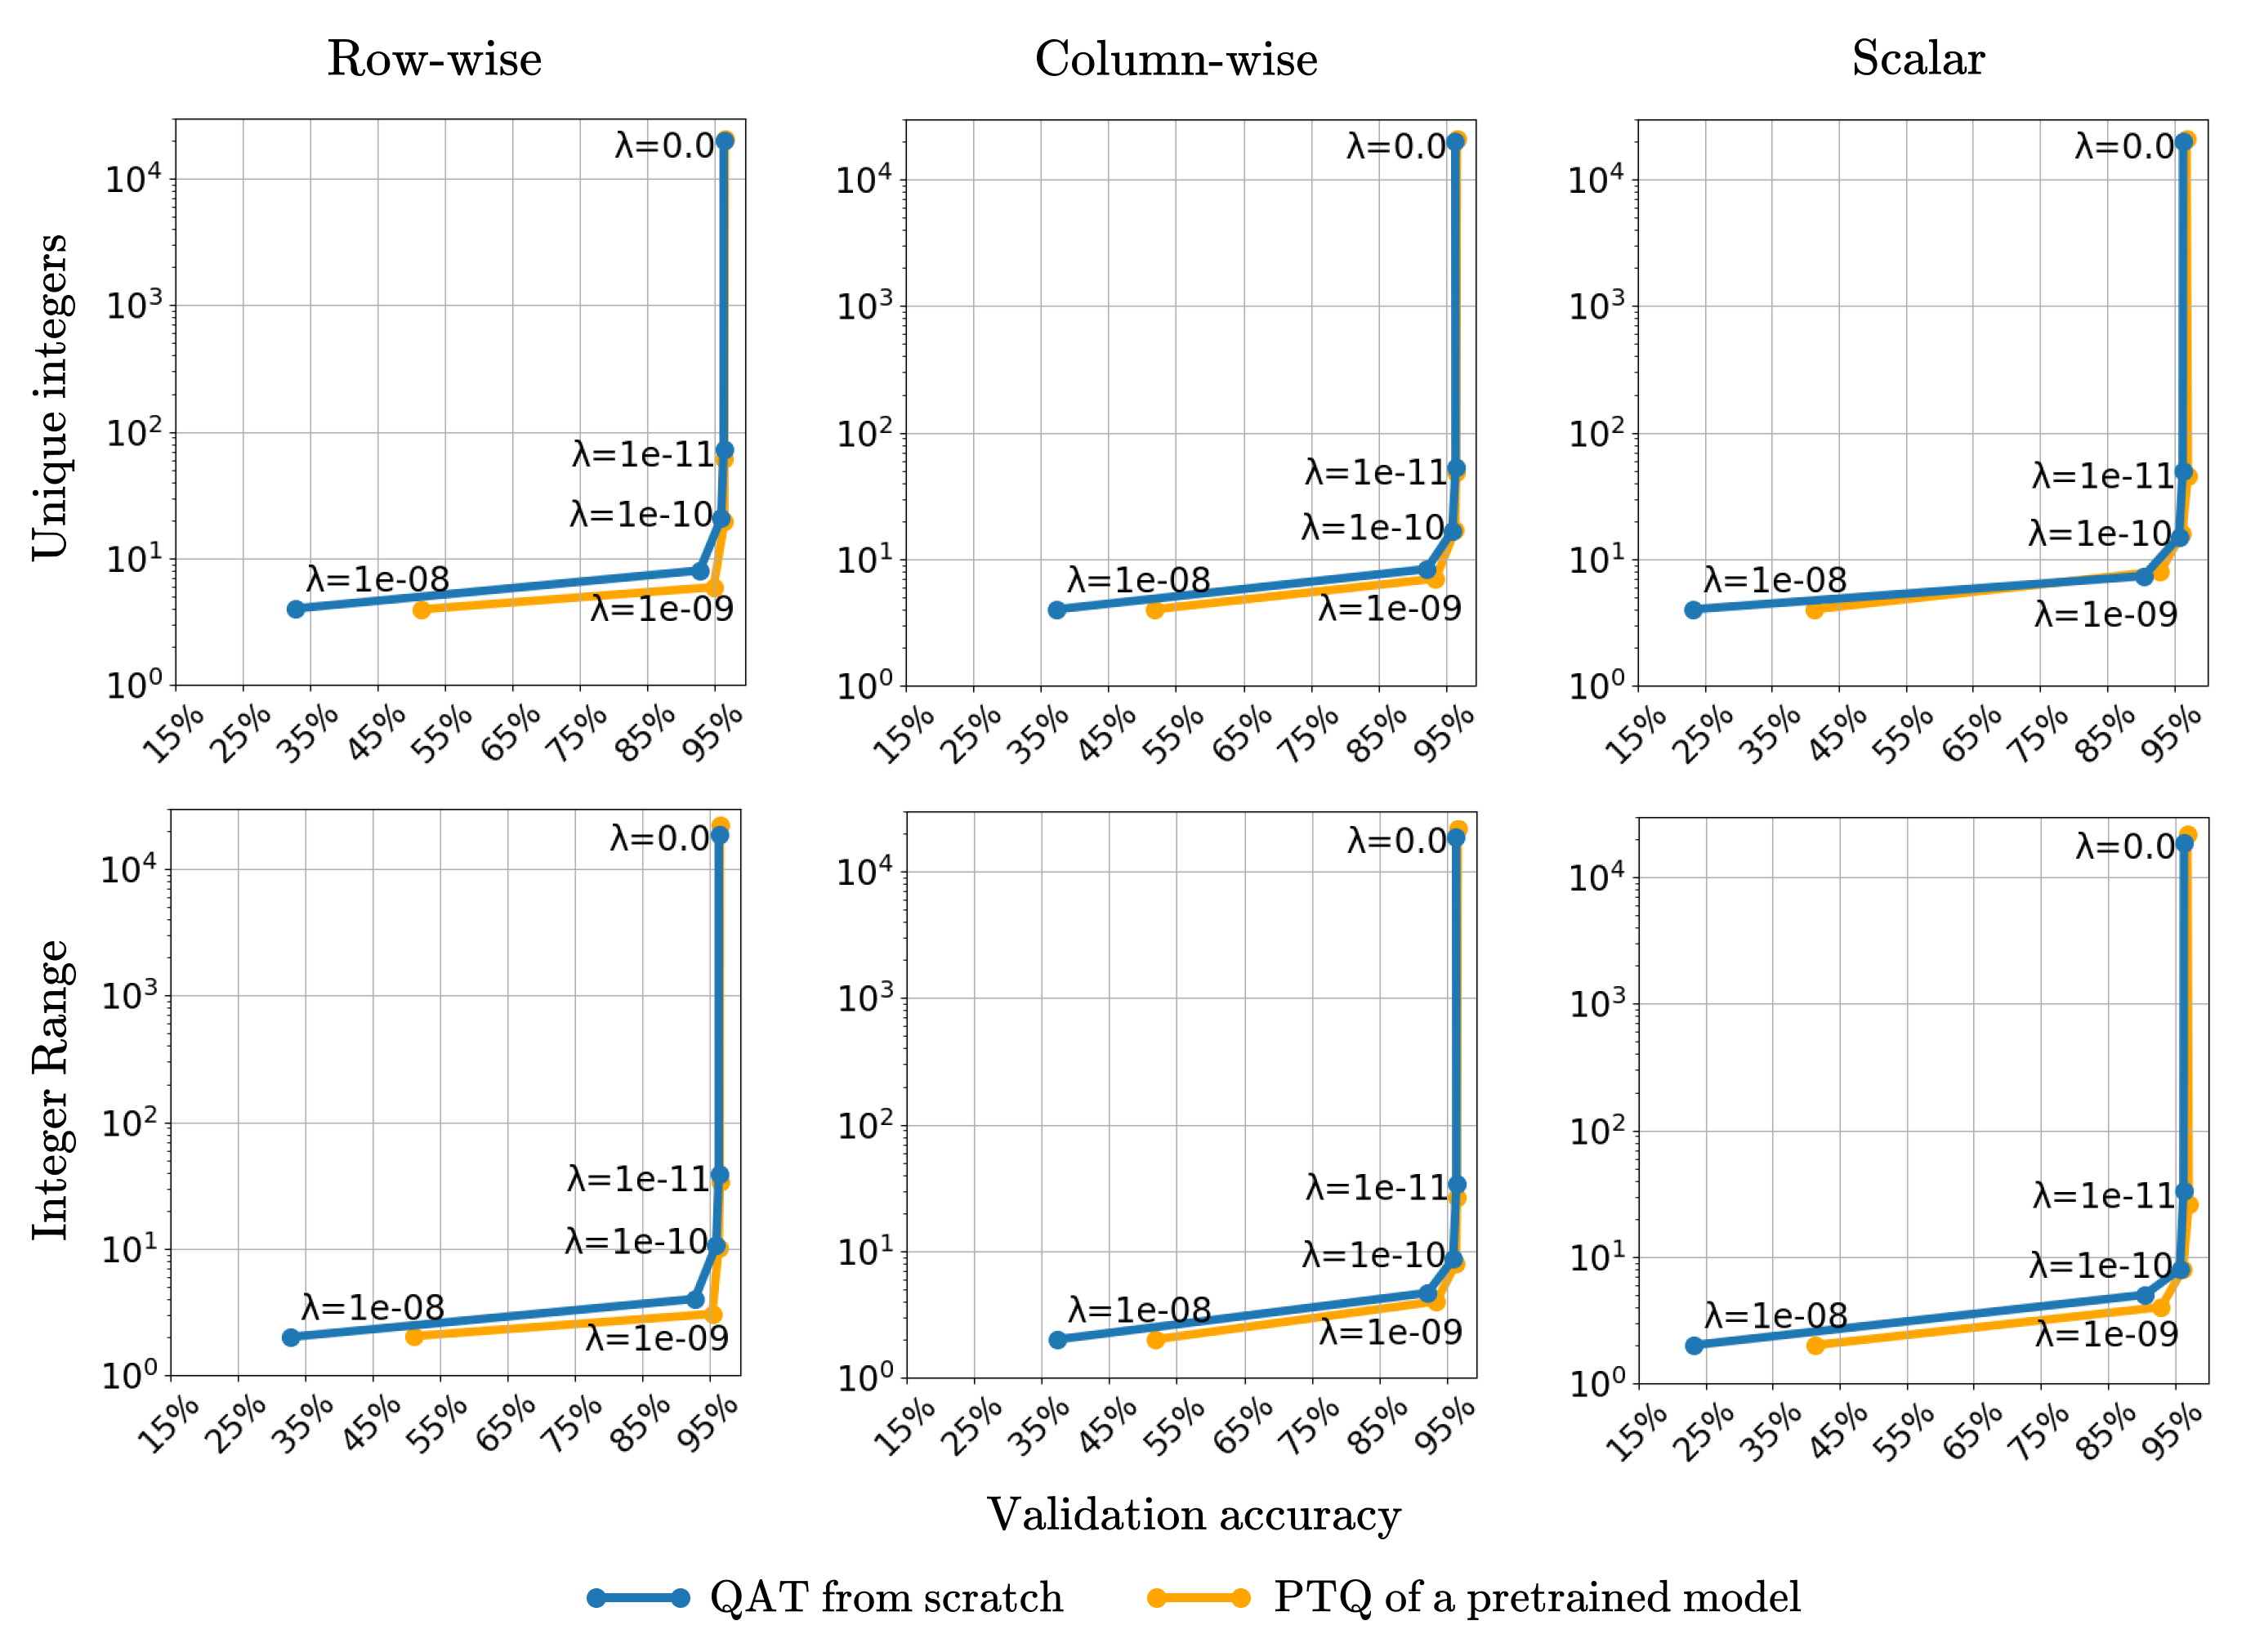
\includegraphics[width=14cm]{pareto-mnist-dense.png}
  \caption{Accuracy – quantization trade-off for nested quantization layers on MNIST.}
  \label{fig:pareto-mnist-dense}
\end{figure}

As an example, the actual integer values after quantization for the rowwise scenario is 
depicted in \cref{fig:quantization_results_1e-10_dense} for all four parameters separately.
While the total number of unique values is only \( 24 \), the range spans from \( -12 \) to \( 11 \).
Consequently, \( 5 \) bits are sufficient to represent the quantized values in the resulting layers, 
as \( \lceil \log_2(24) \rceil = 5 \), covering all 24 unique values within the range. 
The bit requirement can be further reduced using compression techniques like Huffman coding \cite{4051119}, 
considering the concentration of values around 0 in the distributions of quantized weights.


\begin{figure}[b!]
  \centering
  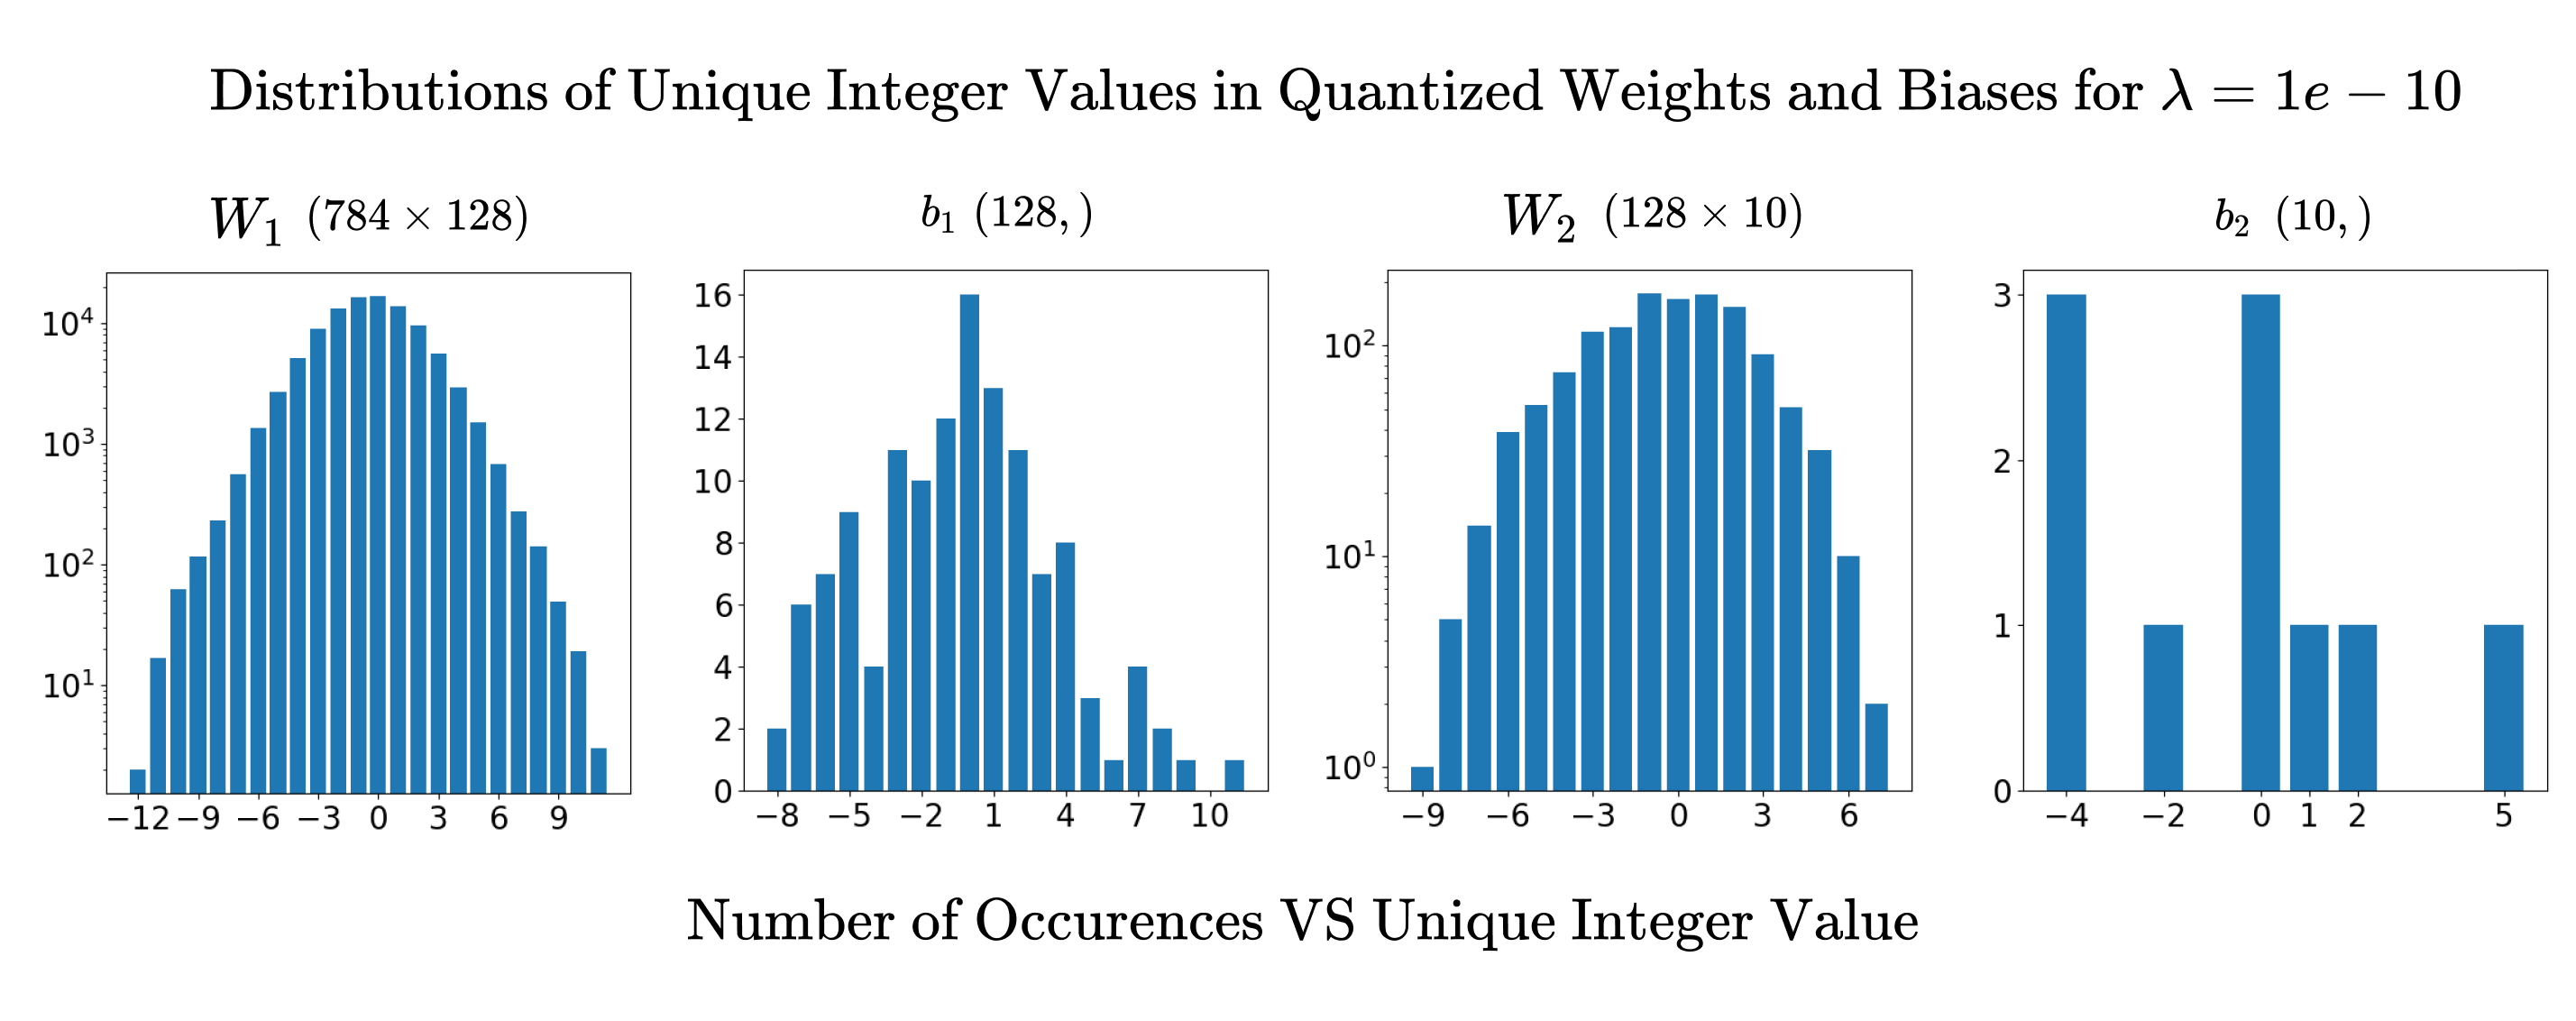
\includegraphics[width=14cm]{quantization_results_1e-10_dense.png}
  \caption{Quantization of MNIST dense layers with row-wise granularity at \( \lambda  = 1e-10 \).}
  \label{fig:quantization_results_1e-10_dense}
\end{figure}


Interestingly, as depicted in \cref{fig:val-accs-over-epochs-dense}, 
the validation loss for \( \lambda = 1e-10 \) 
consistently remains lower than the full-precision baseline and \( \lambda = 0.0 \) throughout the training process.
At the same time, the validation accuracy
remains almost identical to the baseline. This indicates that the penalty threshold of
\( \lambda = 1e-10 \) 
not only preserves the classification accuracy of the model
but also improves generalization with regard to loss,
making the model more confident in its predictions.

\begin{figure}[b!]
  \centering
  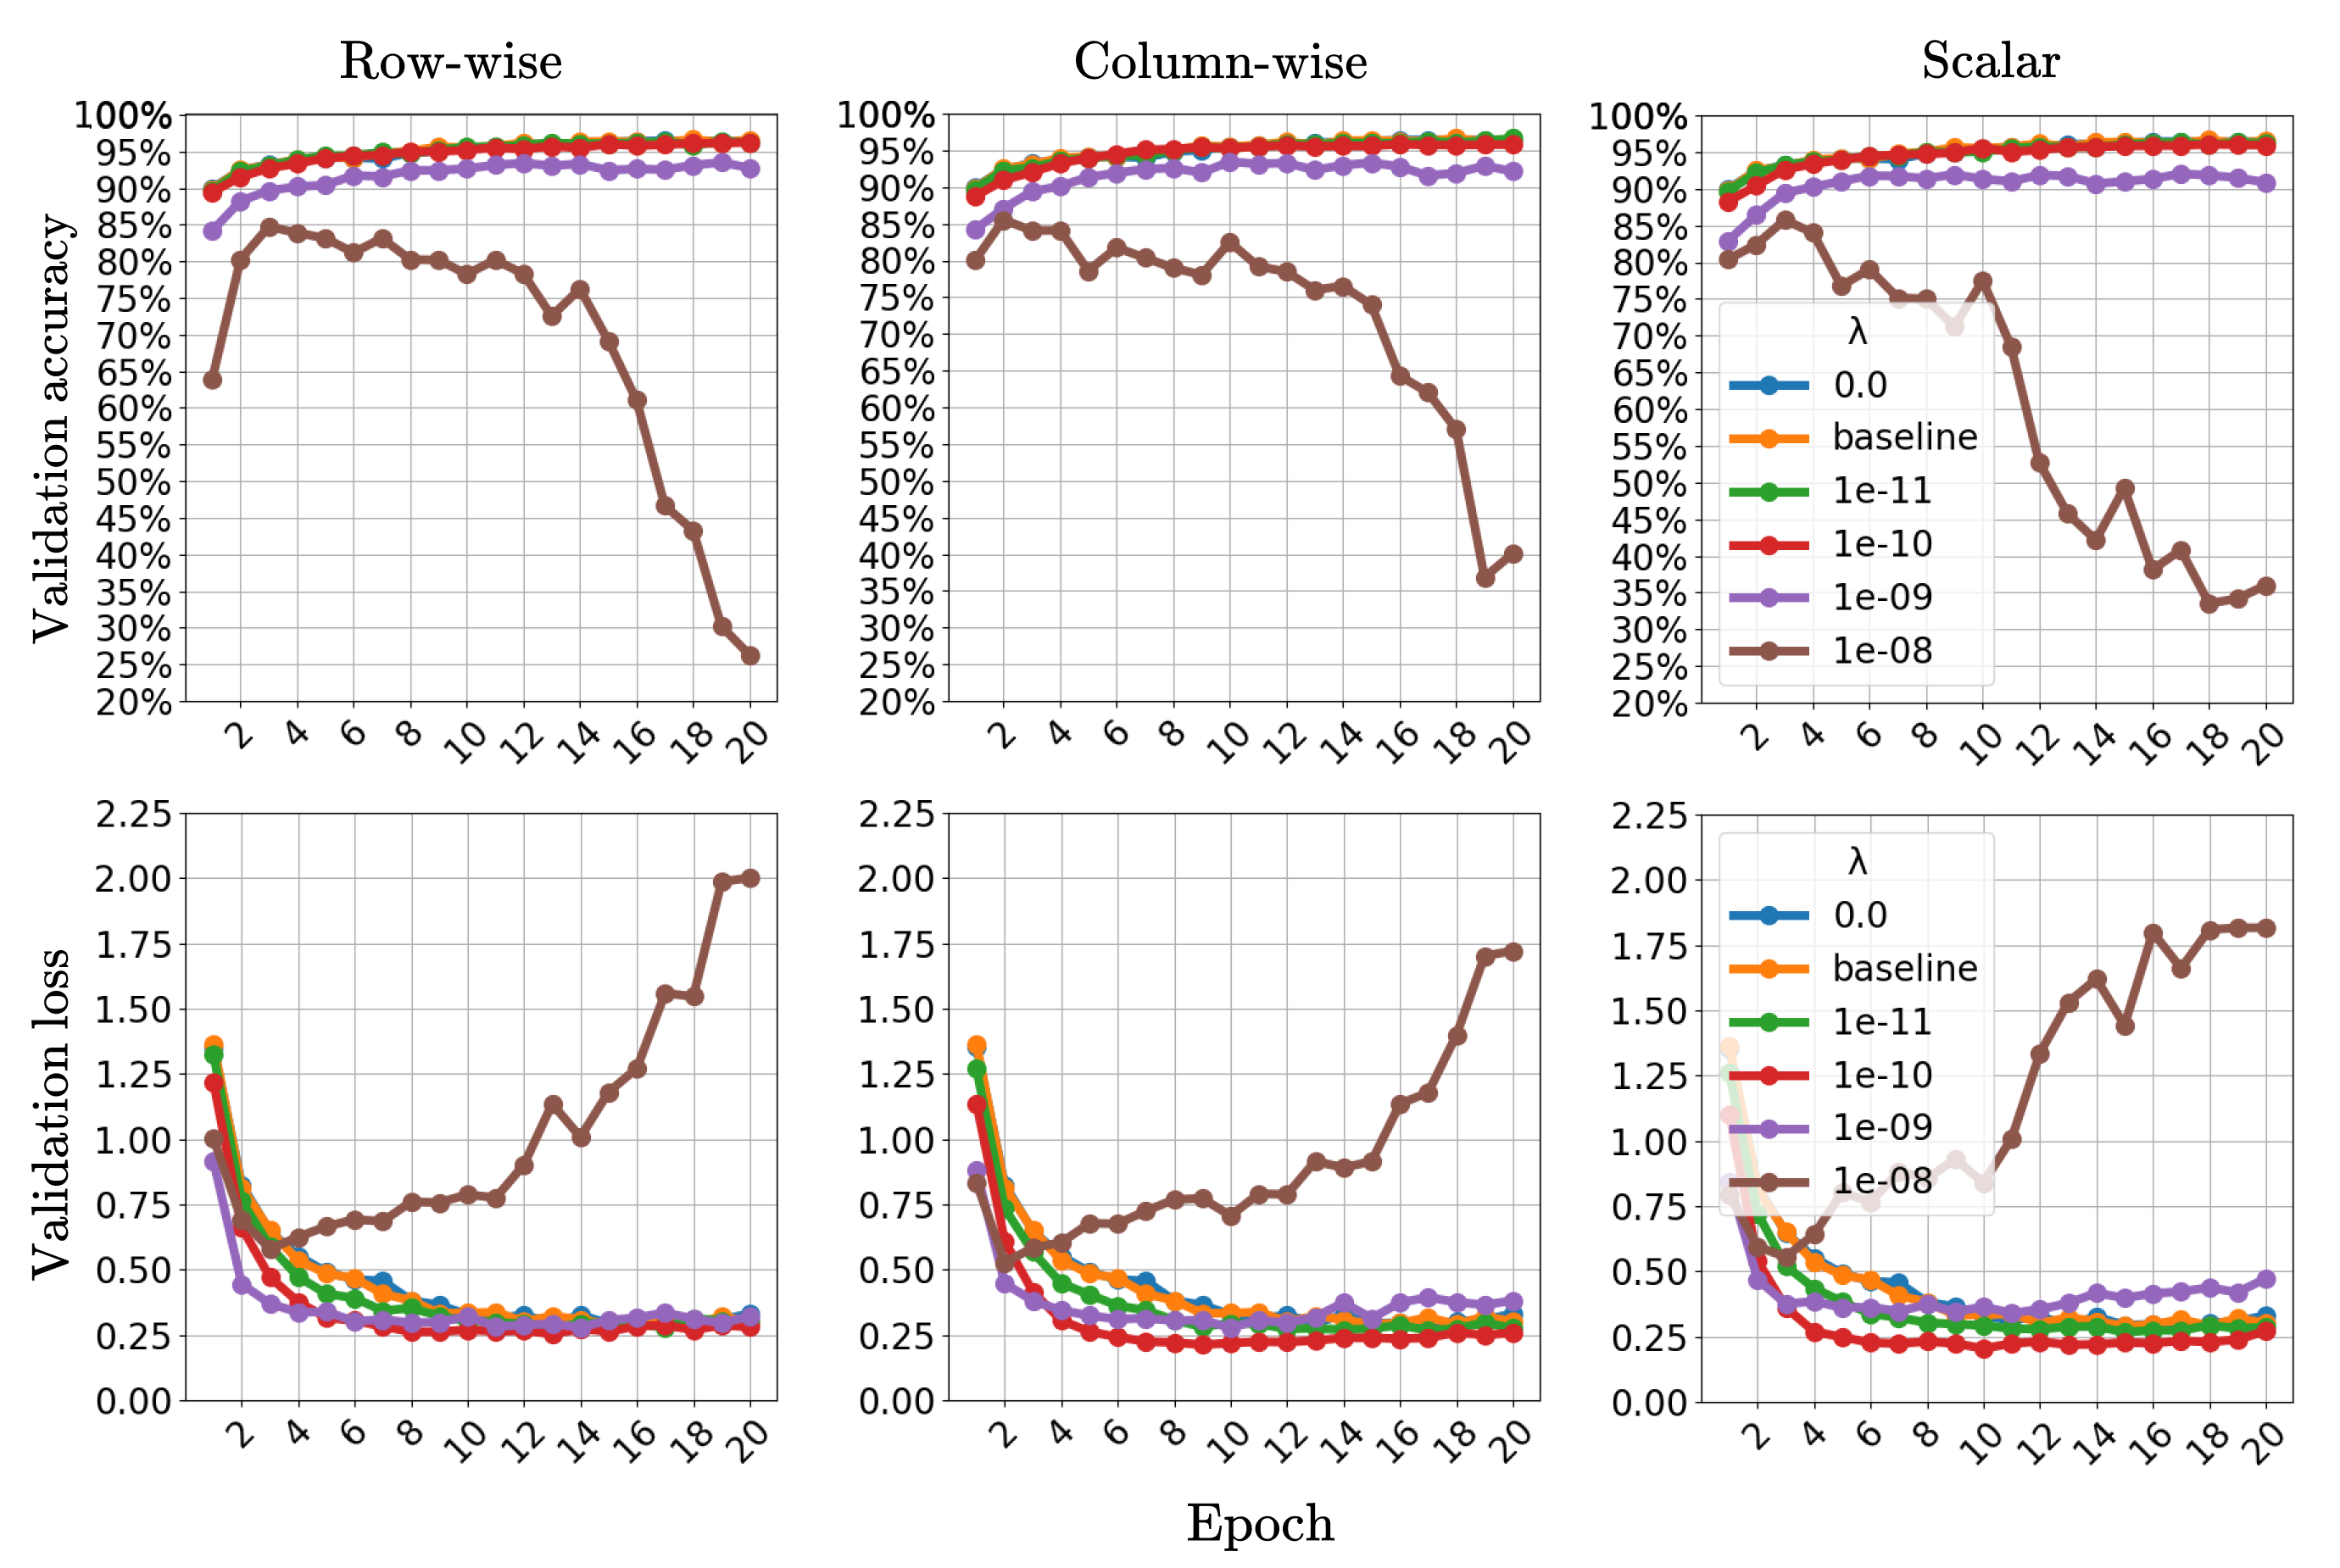
\includegraphics[width=14cm]{dense_nested_val_acc_loss.png}
  \caption{Impact of quantization on accuracy and loss for different \( \lambda \) on MNIST.}
  \label{fig:val-accs-over-epochs-dense}
\end{figure}

In terms of quantization granularity, we see that a scalar scaling factor applied to 
weights produces slightly worse results compared to row-wise and column-wise granularity.
The steeper accuracy degradation and greater loss increase
for \( \lambda = 1e-8\) demonstrate this effect, 
as shown in \cref{fig:val-accs-over-epochs-dense}.
The suboptimal performance of the scalar scaling factor suggests 
that layer-wise quantization, 
which it represents, 
may be too coarse to account for the variability in parameter distributions within a layer.
Therefore, finer granularities, such as row-wise or column-wise scaling, 
are more suitable candidates for optimal quantization granularity of dense layers.

We additionally consider a scenario where the full-precision baseline model is
used to perform post-training quantization (PTQ) with the same set of values for
\( \lambda \). 
In this context, we note that the term PTQ should, in our specific scenario, be extended
to \textit{post-training quantization-aware training}.
However, for simplicity, we continue to use the term PTQ to clearly distinguish this approach from QAT performed from scratch.

As shown
in \cref{fig:pareto-mnist-dense}, we see that the Pareto fronts do not change significantly,
with higher values of \( \lambda \) even achieving a slightly lower number of unique integers at the end
compared to training from scratch.
However, this small advantage is not major. 
As illustrated in \cref{fig:val-accs-over-epochs-dense-pt}, 
this minor benefit occurs only when the model has already lost a significant amount of accuracy.
Nevertheless, the previously defined optimal value of \( \lambda=1e-10 \) holds for PTQ as well,
producing comparable results as shown in \cref{fig:quantization_results_1e-10_dense}

\begin{figure}[b!]
  \centering
  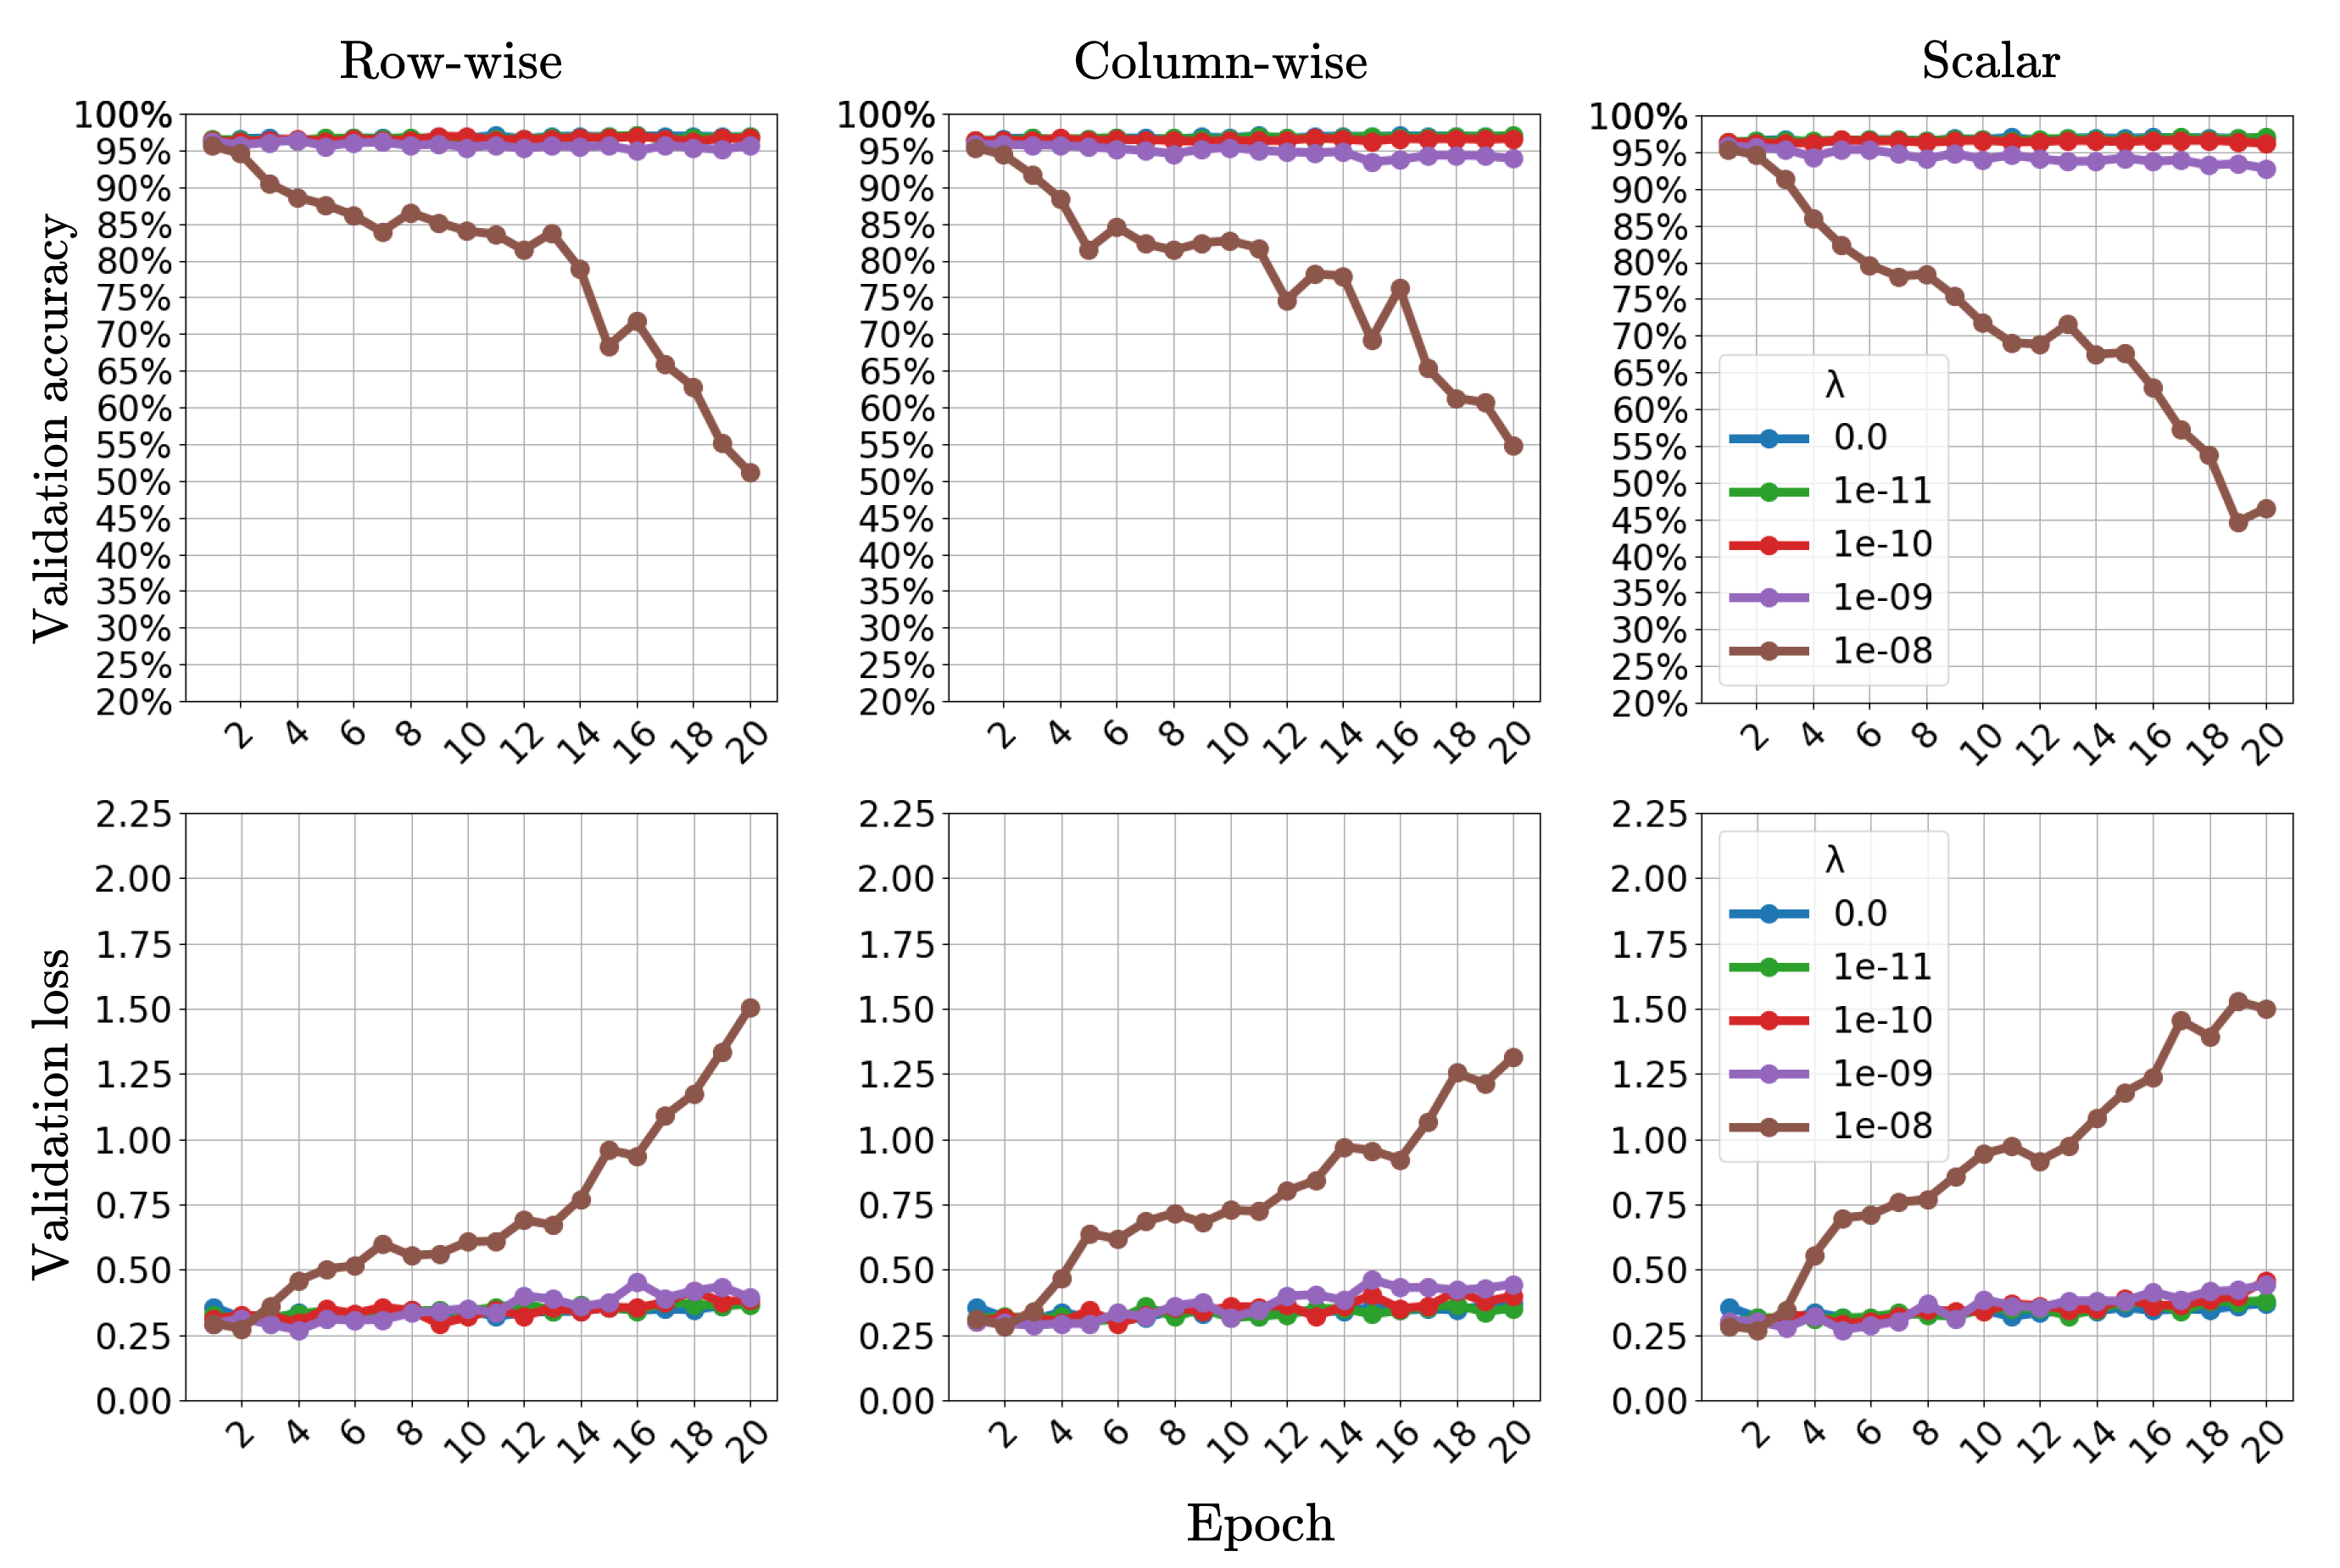
\includegraphics[width=14cm]{dense_nested_val_acc_loss_pt.png}
  \caption{Impact of PTQ on accuracy and loss for different \( \lambda \) on MNIST.}
  \label{fig:val-accs-over-epochs-dense-pt}
\end{figure}

% ----------------------- Nested conv ----------------------- 

\subsection{Convolutional Layers}
\label{subsec:convolutionallayers}
\hspace*{1em}For the CIFAR-10 dataset, we define a CNN, with six nested convolutional layers. 
Each convolutional layer has a kernel and a bias. We examine four scenarios:
applying the scale factor channel-wise, row-wise, column-wise, and as a single
scalar for the entire kernel. For all scenarios, a scalar factor is used for each 
bias vector, similar to how we quantized dense layers. The kernel configurations are shown in
\cref{tab:scalefactorgranularityconv} for clarity.

\begin{table}[t!]
  \centering
  \scriptsize
  \caption{Scale factor granularity for convolutional kernels}
  \label{tab:scalefactorgranularityconv}
  \begin{tabular}{lcccc}
    \toprule
    \textbf{Kernel}                      & \textbf{Channel-wise} & \textbf{Row-wise} & \textbf{Column-wise} & \textbf{Scalar} \\ 
    \midrule
    \( K_{1} \) \( (3, 3, 3, 32) \)     & \( (1, 1, 3, 1) \) & \( (3, 1, 1, 1) \) & \( (1, 3, 1, 1) \) & \( (1, 1, 1, 1) \) \\ 
    \( K_{2} \) \( (3, 3, 32, 32) \)    & \( (1, 1, 32, 1) \) & \( (3, 1, 1, 1) \) & \( (1, 3, 1, 1) \) & \( (1, 1, 1, 1) \) \\ 
    \( K_{3} \) \( (3, 3, 32, 64) \)    & \( (1, 1, 32, 1) \) & \( (3, 1, 1, 1) \) & \( (1, 3, 1, 1) \) & \( (1, 1, 1, 1) \) \\ 
    \( K_{4} \) \( (3, 3, 64, 64) \)    & \( (1, 1, 64, 1) \) & \( (3, 1, 1, 1) \) & \( (1, 3, 1, 1) \) & \( (1, 1, 1, 1) \) \\ 
    \( K_{5} \) \( (3, 3, 64, 128) \)   & \( (1, 1, 64, 1) \) & \( (3, 1, 1, 1) \) & \( (1, 3, 1, 1) \) & \( (1, 1, 1, 1) \) \\ 
    \( K_{6} \) \( (3, 3, 128, 128) \)  & \( (1, 1, 128, 1) \) & \( (3, 1, 1, 1) \) & \( (1, 3, 1, 1) \) & \( (1, 1, 1, 1) \) \\ 
    \bottomrule
  \end{tabular}
  \vspace{0.5em}
  \caption*{\footnotesize Note: \( (1, 1, 1, 1) \) denotes a scalar, broadcasted across the kernel for consistency.}
\end{table}

The experiments show that the optimal value for the hyperparameter is \( \lambda = 1e-11\),
across all four scenarios, as depicted in \cref{fig:pareto-cifar-conv}.
\begin{figure}[b!]
  \centering
  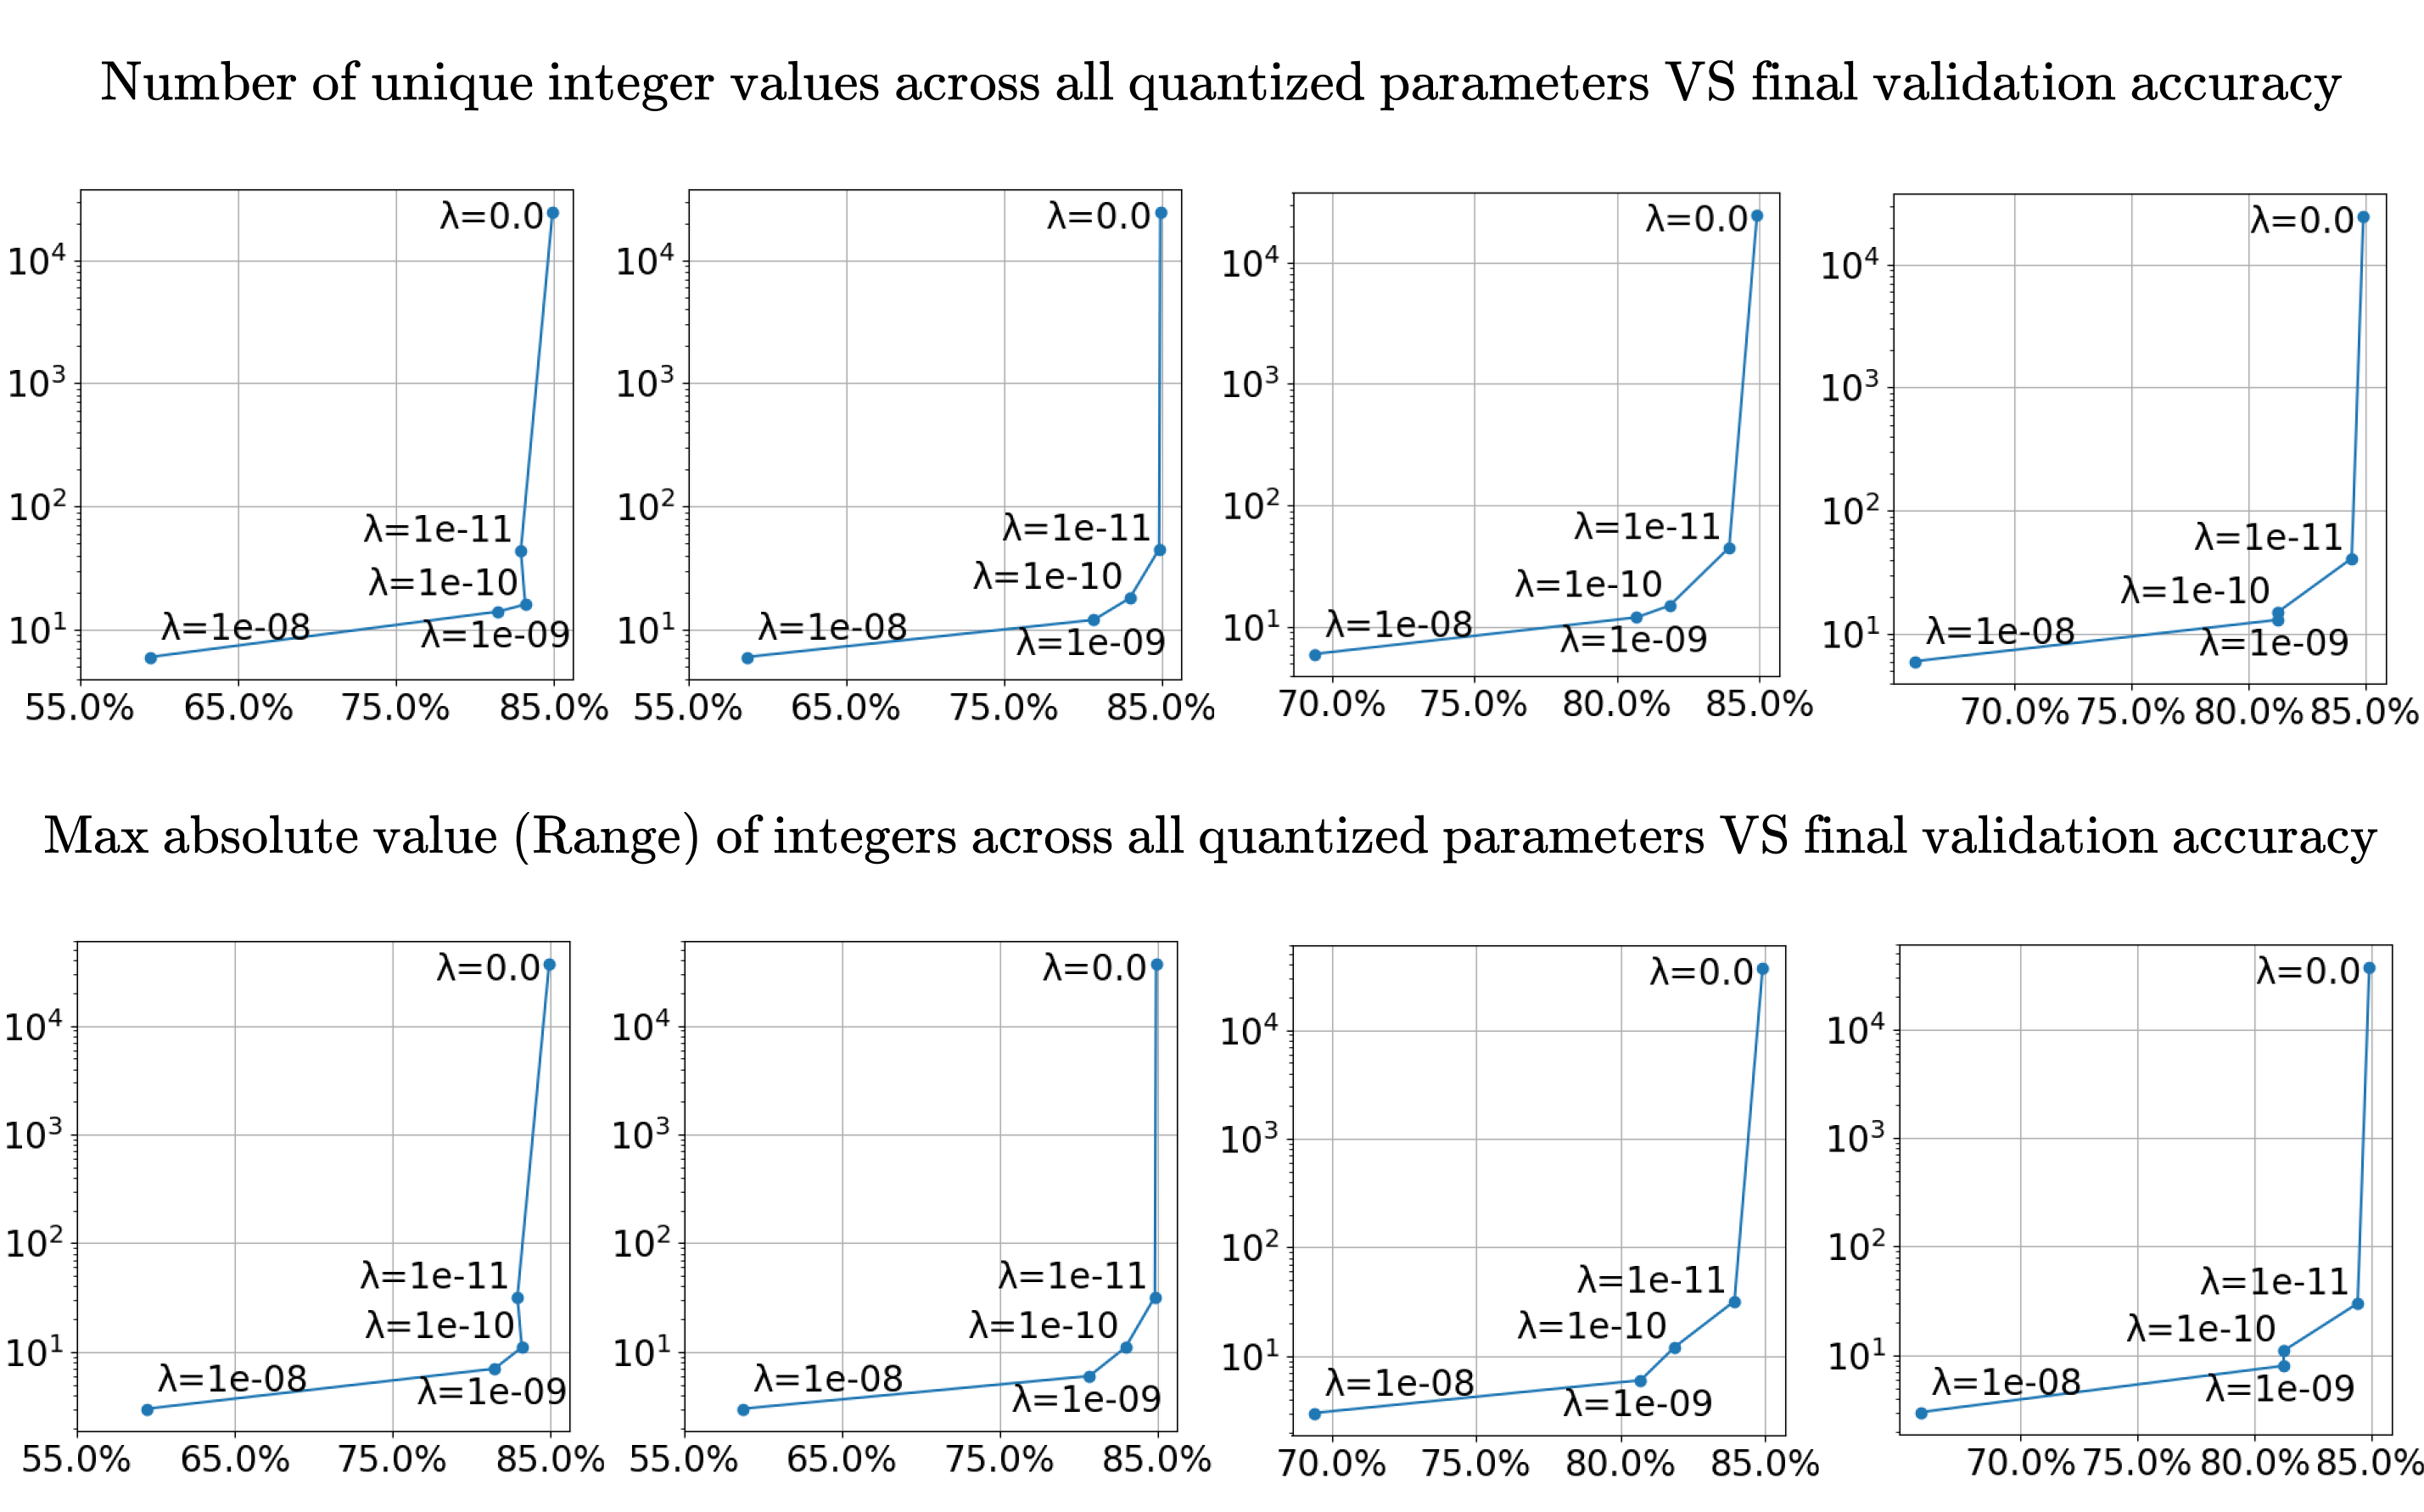
\includegraphics[width=14cm]{pareto-cifar-conv.png}
  \caption{Accuracy–quantization trade-off for nested quantization layers on CIFAR-10.}
  \label{fig:pareto-cifar-conv}
\end{figure}
As an example, the integer values after quantization for the row-wise scenario across
all quantized parameters range from \( -22 \) to \( 32 \), 
resulting in \( 60 \) unique values that can be represented with \( \lceil \log_2(60) \rceil = 6 \) bits.
The histograms of the resulting integer values in the kernels, displayed in \cref{fig:quantization-results-1e-10conv},
form a bell curve similar to the experimental results for dense layer weights.
\begin{figure}[t!]
  \centering
  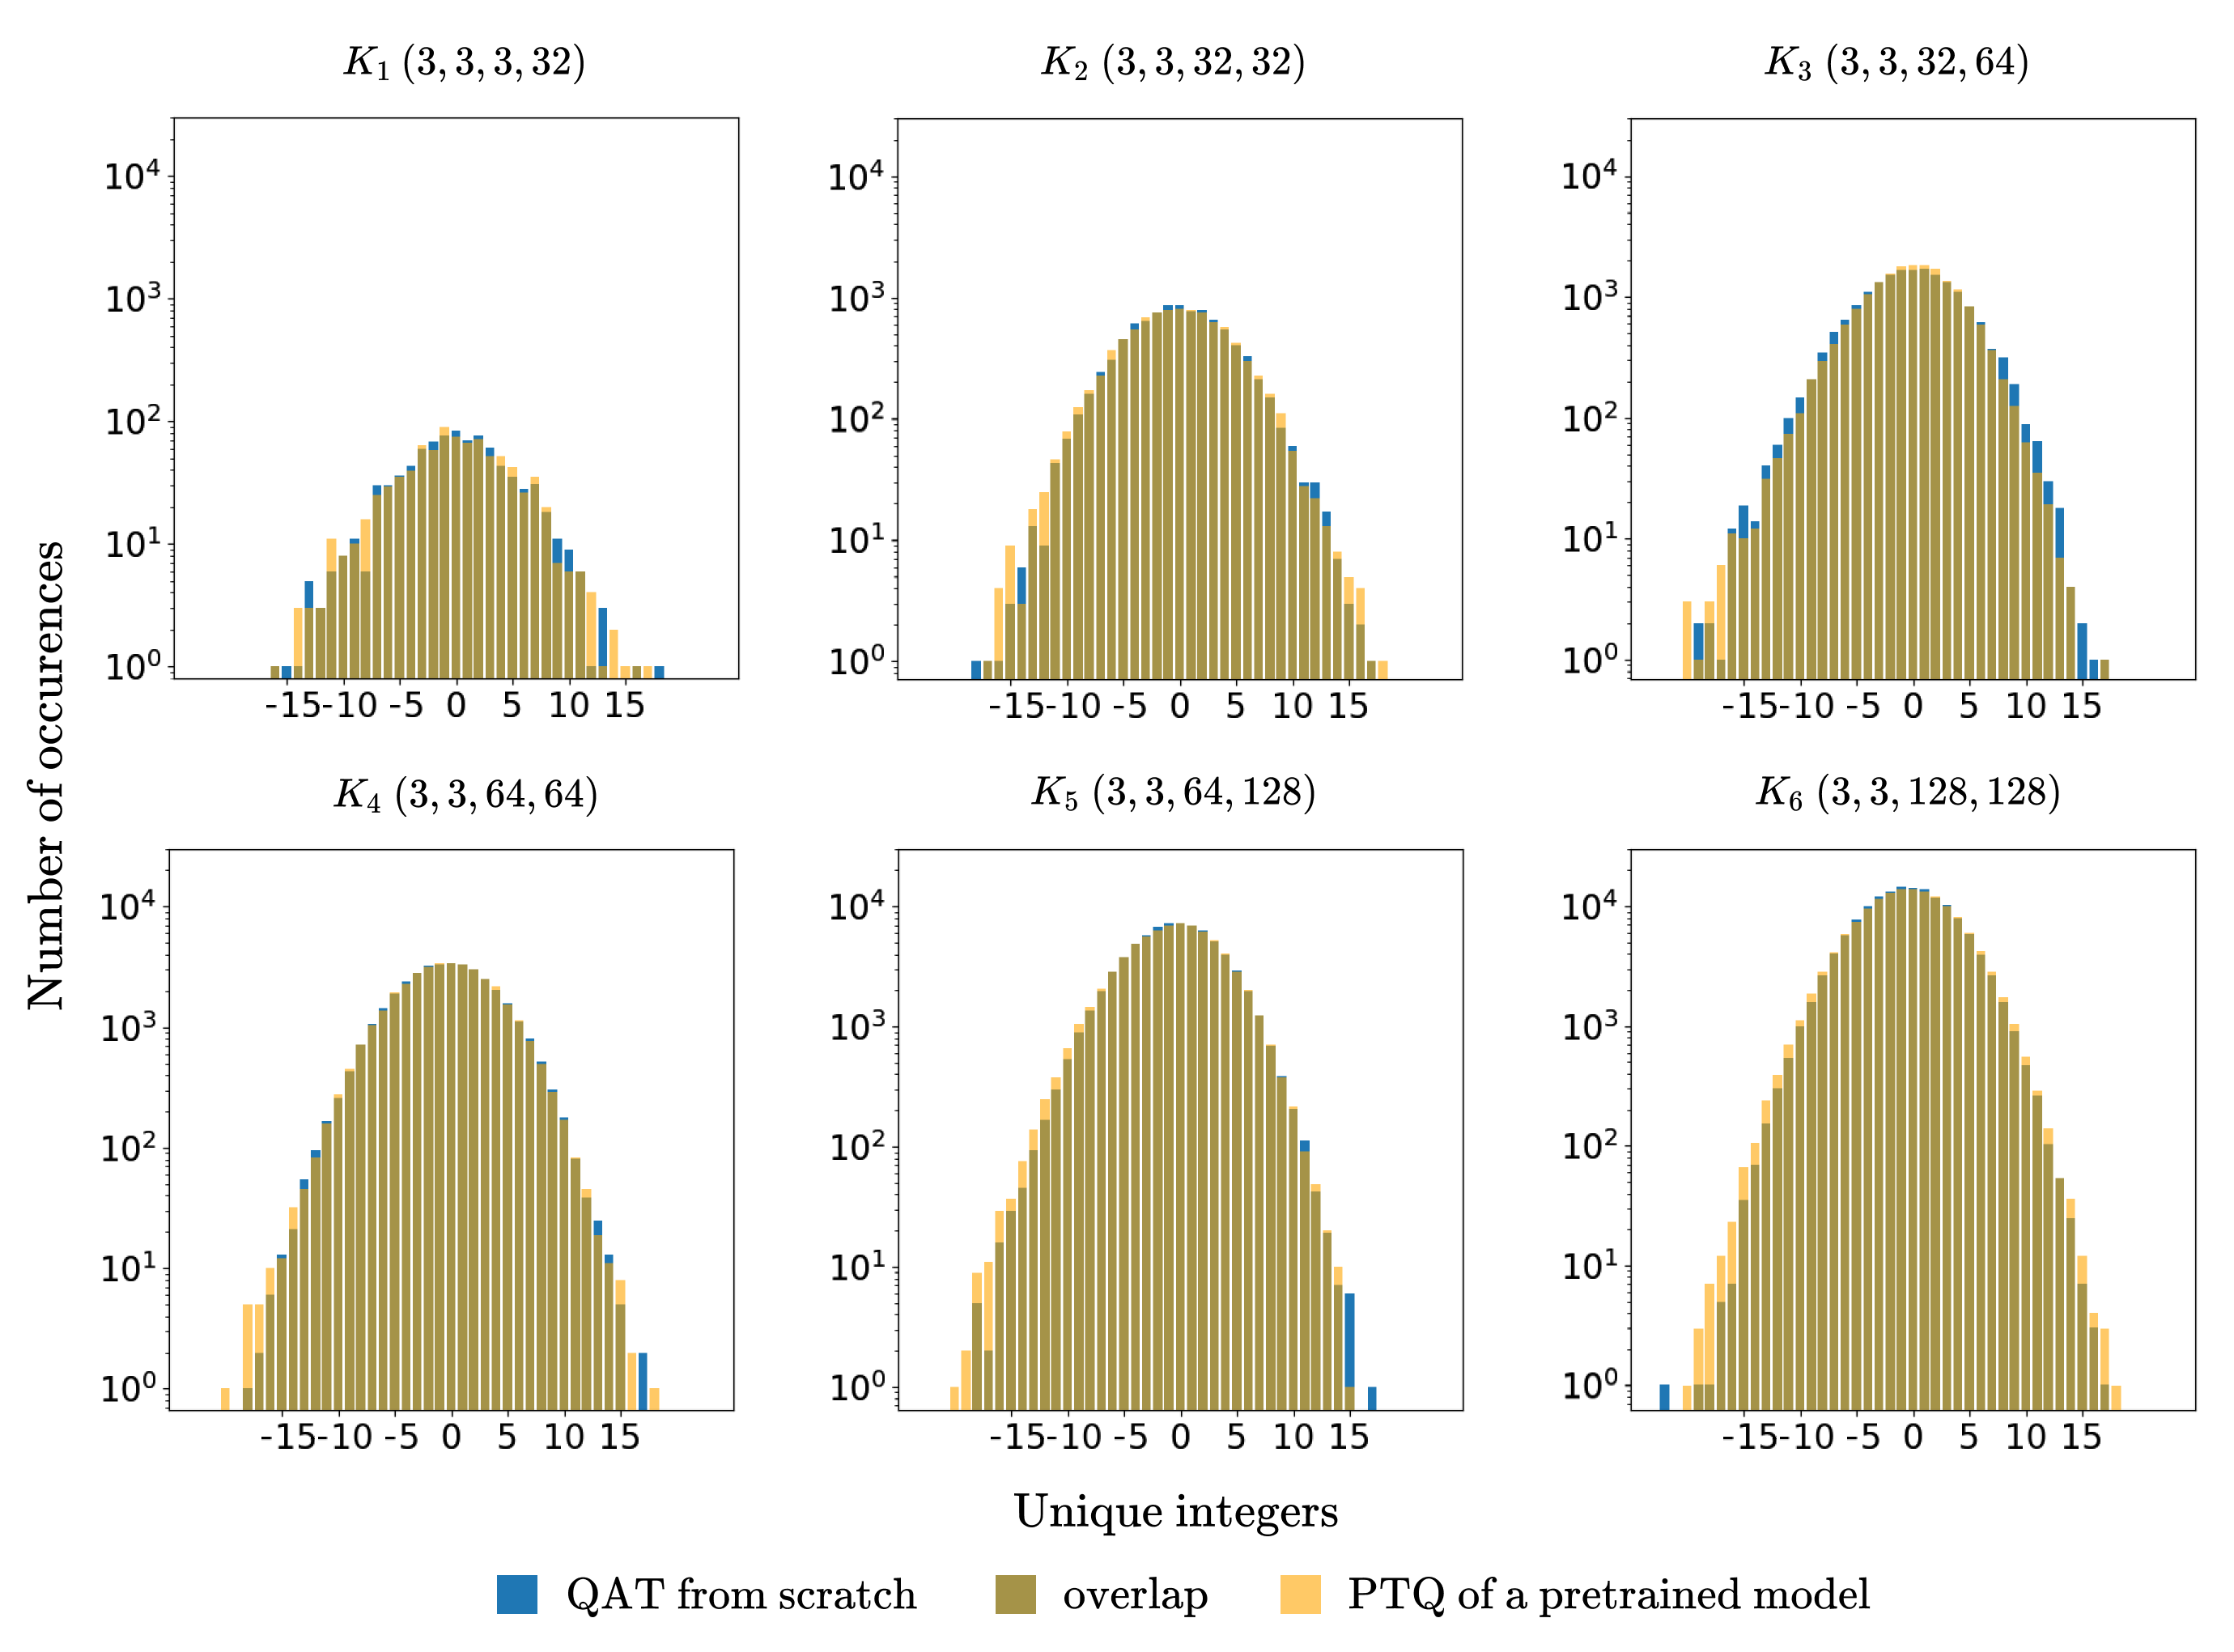
\includegraphics[width=14cm]{quantization_results_1e-11_conv.png}
  \caption{Quantization of CIFAR-10 kernels with row-wise granularity at  \( \lambda  = 1e-11 \).}
  \label{fig:quantization-results-1e-10conv}
\end{figure}
\begin{figure}[t!]
  \centering
  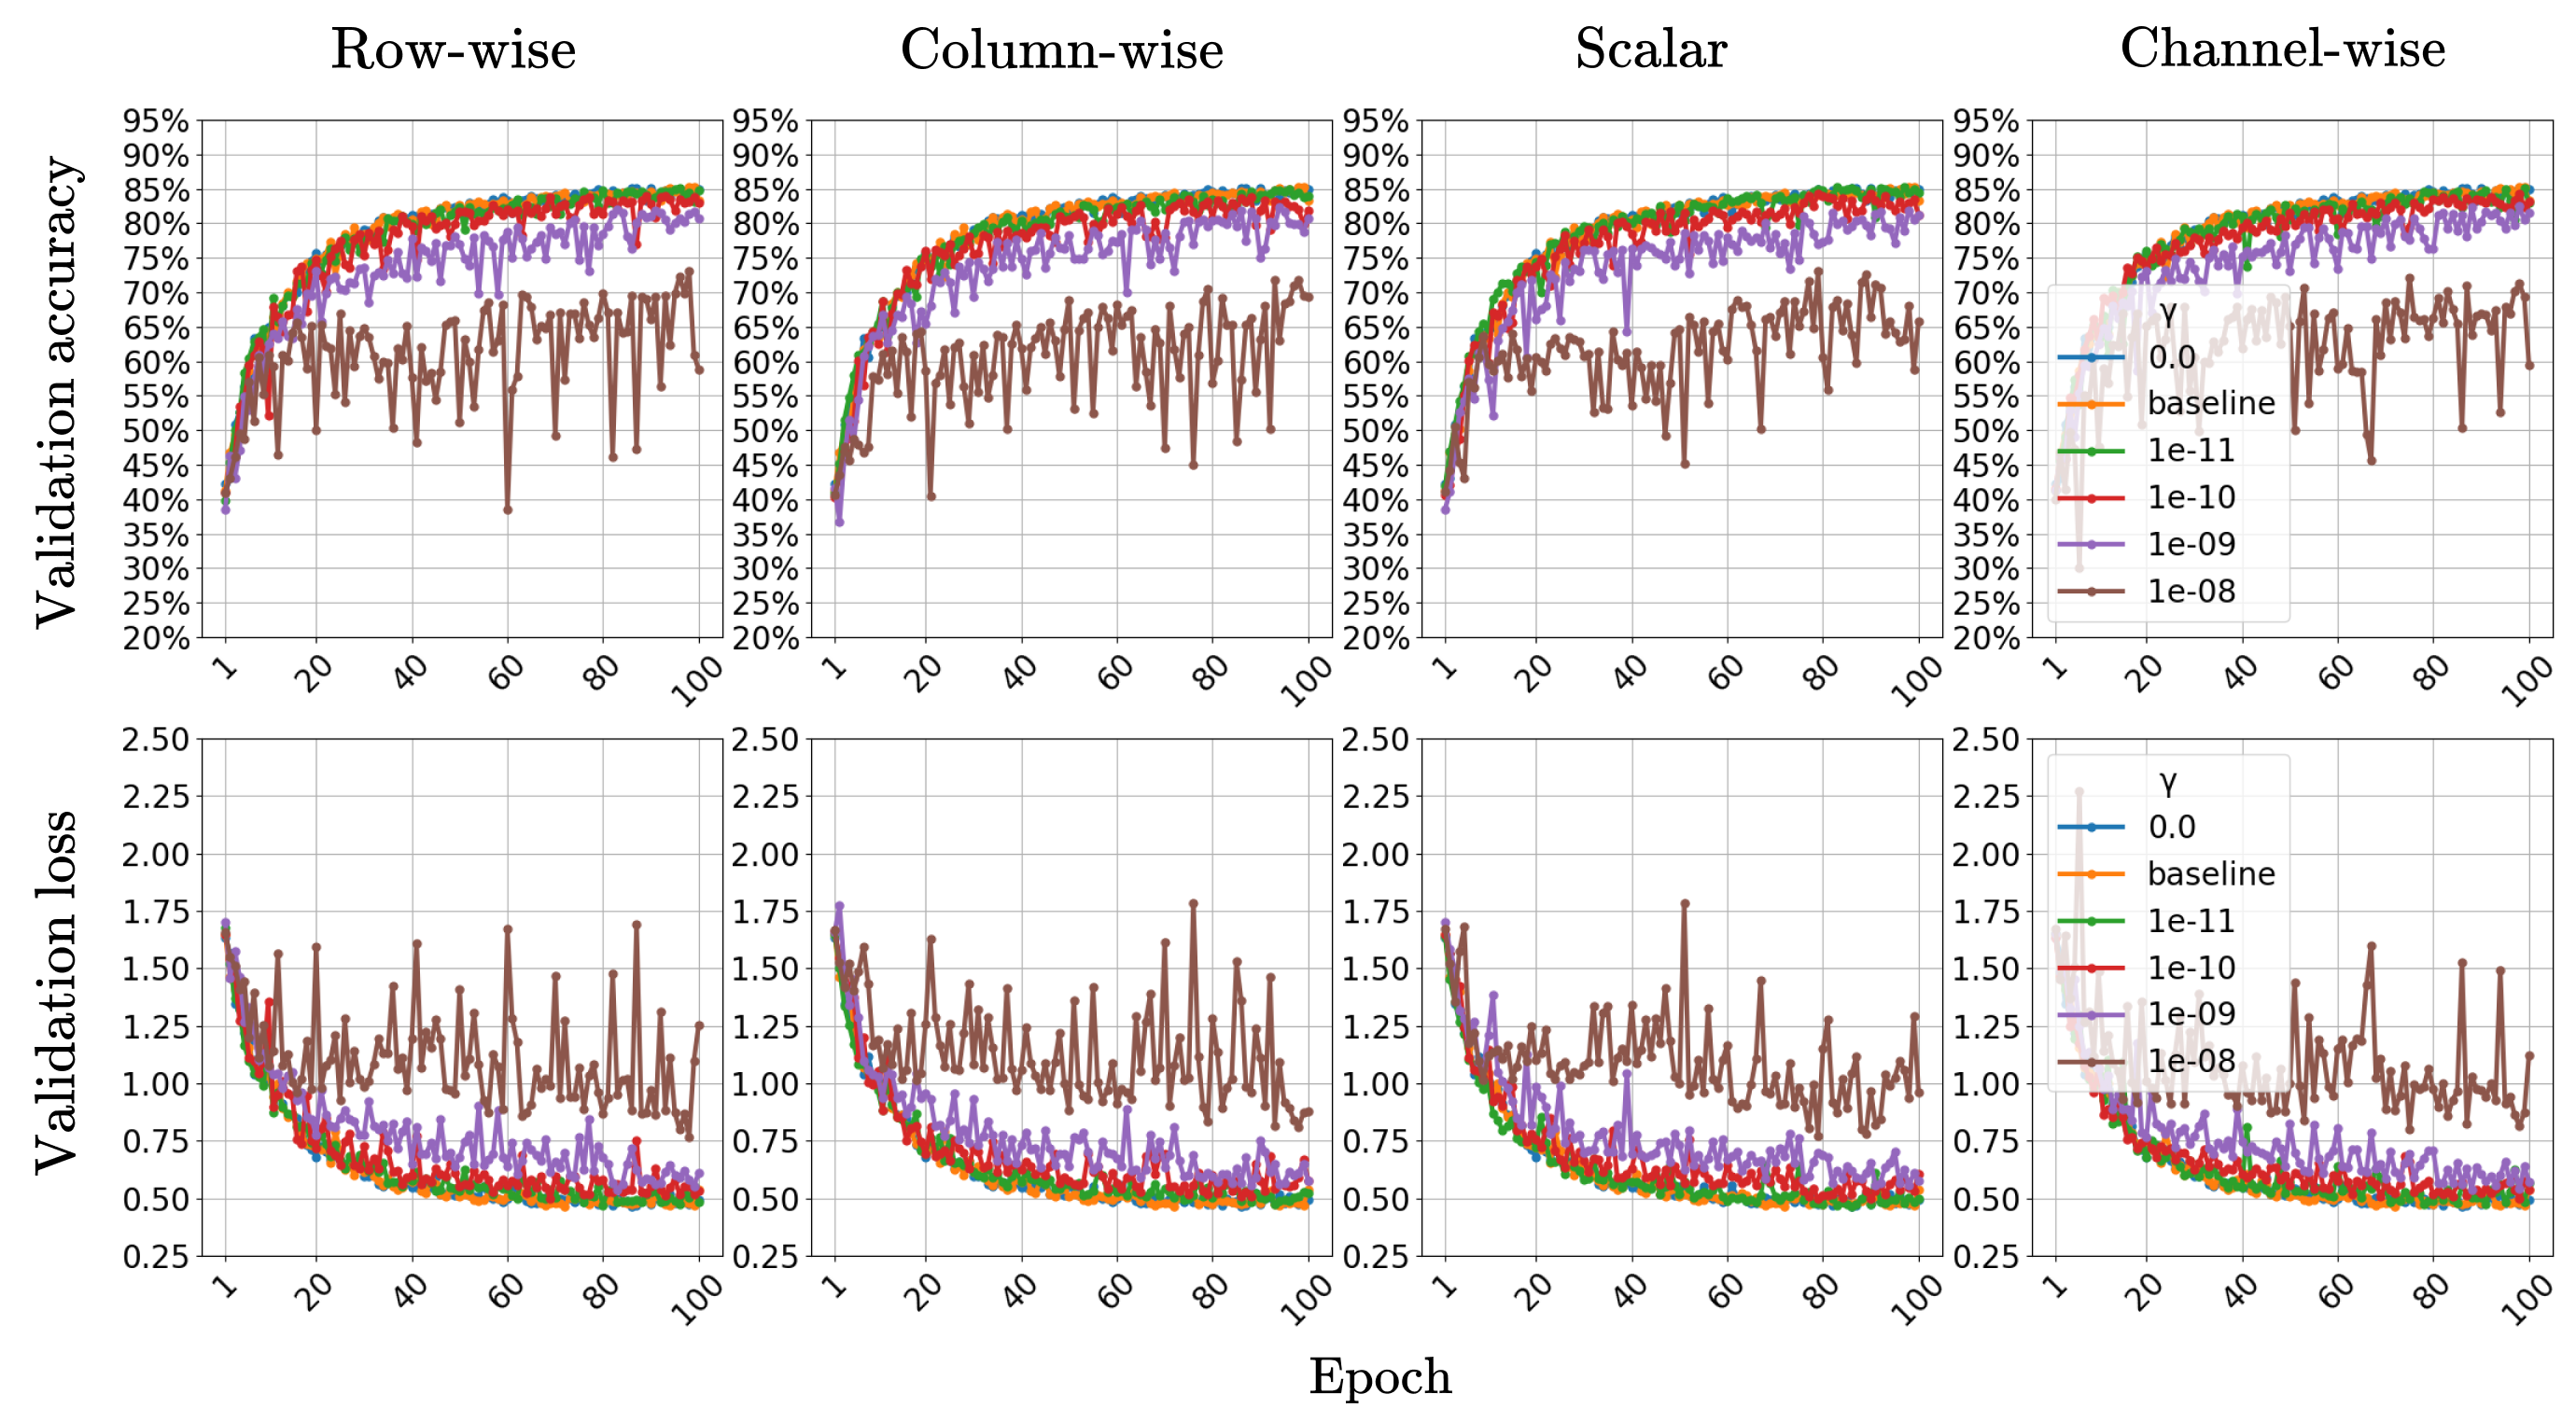
\includegraphics[width=14cm]{conv_nested_val_acc_loss.png}
  \caption{Impact of quantization on accuracy and loss for different \( \lambda \) on CIFAR-10.}
  \label{fig:val-accs-over-epochs-conv}
\end{figure}
If a slightly greater degradation in accuracy is viable, 
\( \lambda \) can be increased to \( \lambda = 1e-10\).
In the row-wise case, this adjustment results in a reduced range of integers,
spanning from \( -8 \) to \( 11 \). Further increasing \( \lambda \) could
reduce the number of unique values to less than ten.

\begin{table}[b!]
  \centering
  \caption{Compression rate of the nested quantization layer method}
  \label{tab:nestedcomrpessionrate}
  \begin{tabular}{lccc}
      \toprule
      \textbf{Dataset}     & \textbf{Baseline} & \textbf{PTQ + Compression} & \textbf{Granularity, $\lambda$} \\ 
      \midrule
      MNIST                & $\approx 0.36 $ MB            & $\approx 0.05 $ MB              & row-wise, $1e-10$         \\ 
      CIFAR-10          &  $\approx 1.02 $ MB          & $\approx 0.16 $ MB            & row-wise, $1e-11$            \\ 
      Imagenette               &  $\approx 39.57 $ MB          & $\approx 6.39 $ MB             & channel-wise, $1e-11$          \\ 

      \bottomrule
  \end{tabular}
  \vspace{0.5em}
\end{table}


\begin{figure}[t!]
  \centering
  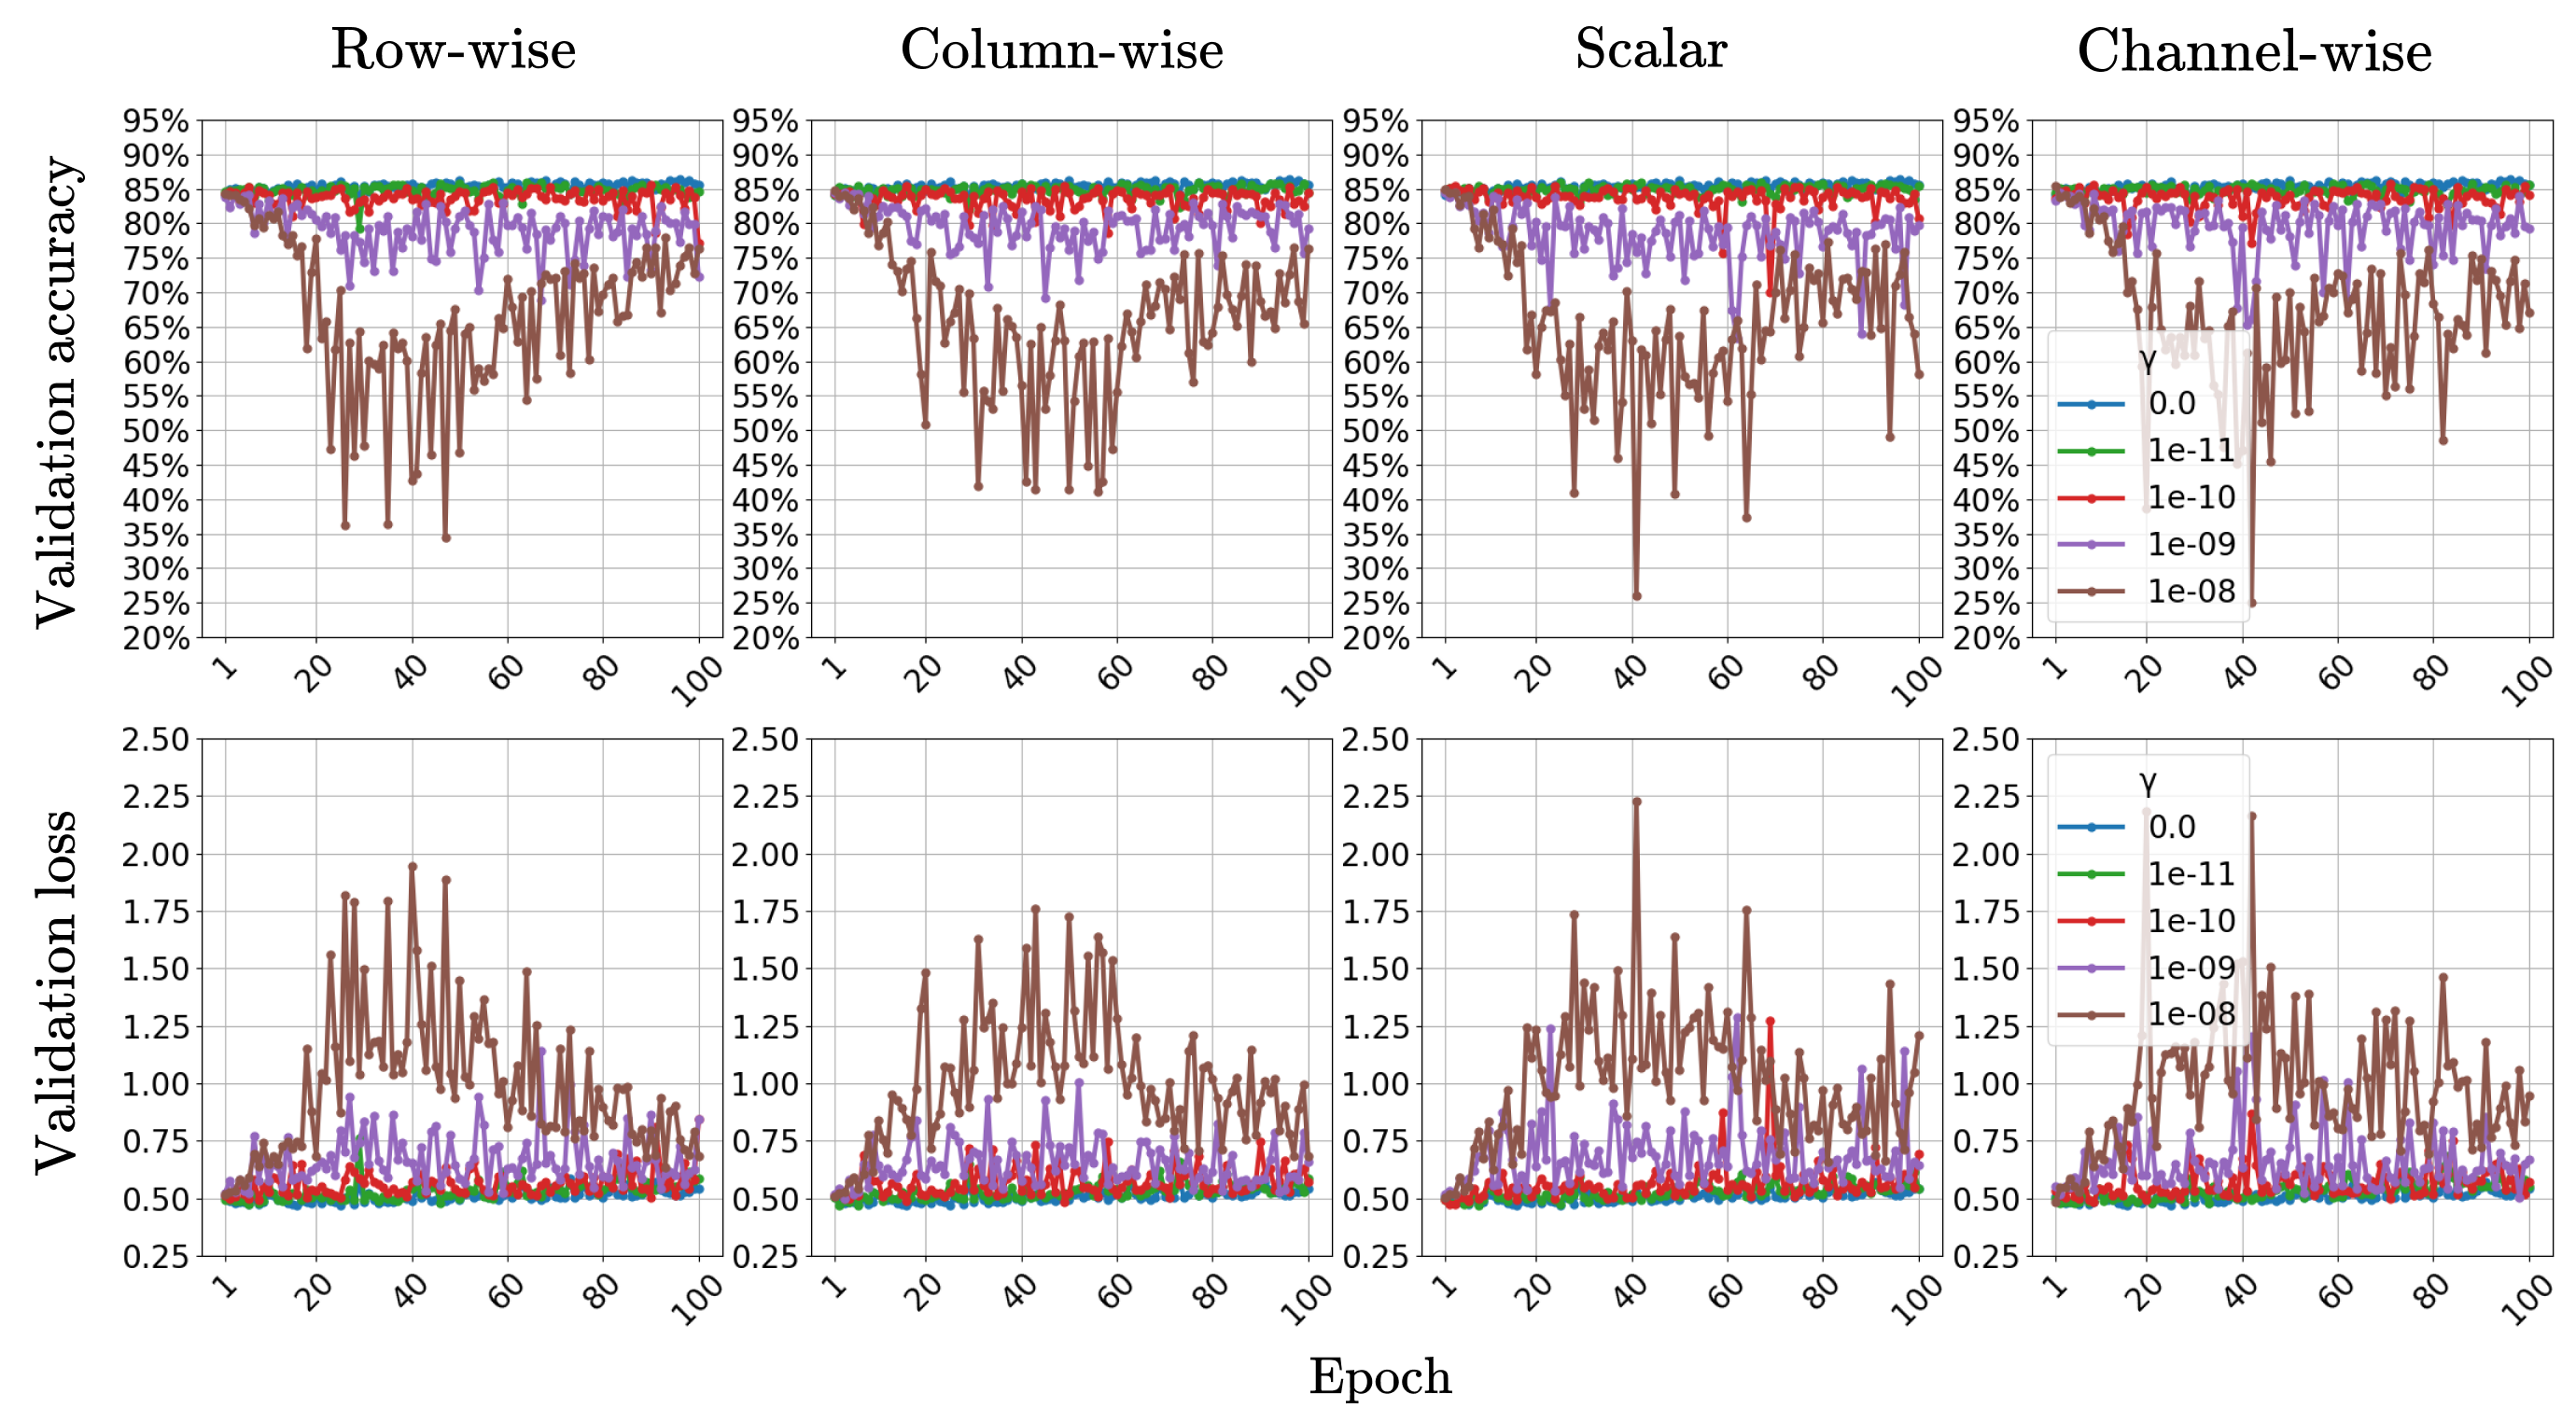
\includegraphics[width=14cm]{conv_nested_val_acc_loss_pt.png}
  \caption{Impact of PTQ on accuracy and loss for different \( \lambda \) on CIFAR-10.}
  \label{fig:val-accs-over-epochs-conv-pt}
\end{figure}

From \cref{fig:val-accs-over-epochs-conv}, 
we do not observe a significant difference in performance between the row-wise, 
column-wise, channel-wise, 
and scalar granularity scenarios. 
This suggests that the gradient-based method for updating scale factors produces 
"votes" and aggregated updates that are largely consistent across granularities. 
As a result, the scale factors tend to converge to similar values. 
Therefore, the scalar granularity may be the most suitable choice, 
as it requires the fewest parameters and offers the simplest implementation.
\newpage
In PTQ, we achieve results similar to those observed in dense layers, as shown in
\cref{fig:pareto-cifar-conv} and \cref{fig:quantization-results-1e-10conv}.
However, the validation loss progression during PTQ, demonstrated in \cref{fig:val-accs-over-epochs-conv-pt},
shows an interesting pattern for  \( \lambda = 1e-8\).
We observe that the validation loss increases initially but decreases towards the end. 
This stabilization occurs when the model reaches a significant level of quantization
— indicated by \( m \) (introduced in \cref{subsec:learnedscalefactor}), the maximum integer value for a given scale factor, becoming very small.
As  \( m \) drops, the gradient updates for the corresponding scale factor also shrink, 
causing the scale factors to converge. Such convergence, in its turn, helps the pretrained
model to re-stabilize. These observations suggest that the gradient-based approach 
may also be effective for PTQ scenarios where pretrained models need to be quantized.

For the Imagenette dataset, 
we define a ResNet-inspired network with twenty convolutional layers. 
Similarly, we examine four scenarios, each corresponding to different granularities.
While the specific kernel sizes differ, the logic for assigning scale factor configurations 
follows the same approach as outlined in \cref{tab:scalefactorgranularityconv}.
\newpage
The resulting Pareto front plots are depicted in \cref{fig:imagenette-nested}, 
where we see that PTQ has yielded significant accuracy improvement. 
This improvement is connected to the learning rate decay. Specifically, when we take a pretrained model that
ended its training with a very low learning rate and begin retraining to quantize with a larger learning rate,
the model essentially becomes more flexible, accommodating further convergence.

Similar to the observations on CIFAR-10, we do not see a significant difference between various granularity settings applied to Imagenette convolutional layers.


\cref{tab:nestedcomrpessionrate} presents the compressed file sizes of dense or convolutional layers before and after applying our PTQ in selected scenarios. 
To ensure a fair comparison, the Baseline column reflects the size of the original, unquantized FP32 weights and biases, which are compressed using zipping. 
The PTQ + Compressed column, on the other hand, shows the size after quantization and compression.

Specifically, the quantization and compression process involves flooring the weights and biases to
INT8 format, saving them as \texttt{.npy} files, and subsequently compressing these files using zipping. 
It is important to note that this compression method is intended solely for demonstration purposes, 
to highlight the potential reduction gains, and does not necessarily represent an efficient deployment format.

Across the three datasets, we observe up to an eight-fold reduction in file size.
We also note that the scaling factors must be saved separately in FP32, 
since they are used during the forward-pass to rescale the weights and biases. 
However, these full-precision scale factors are relatively small, so their storage overhead is minimal.


\begin{figure}[t!]
  \centering
  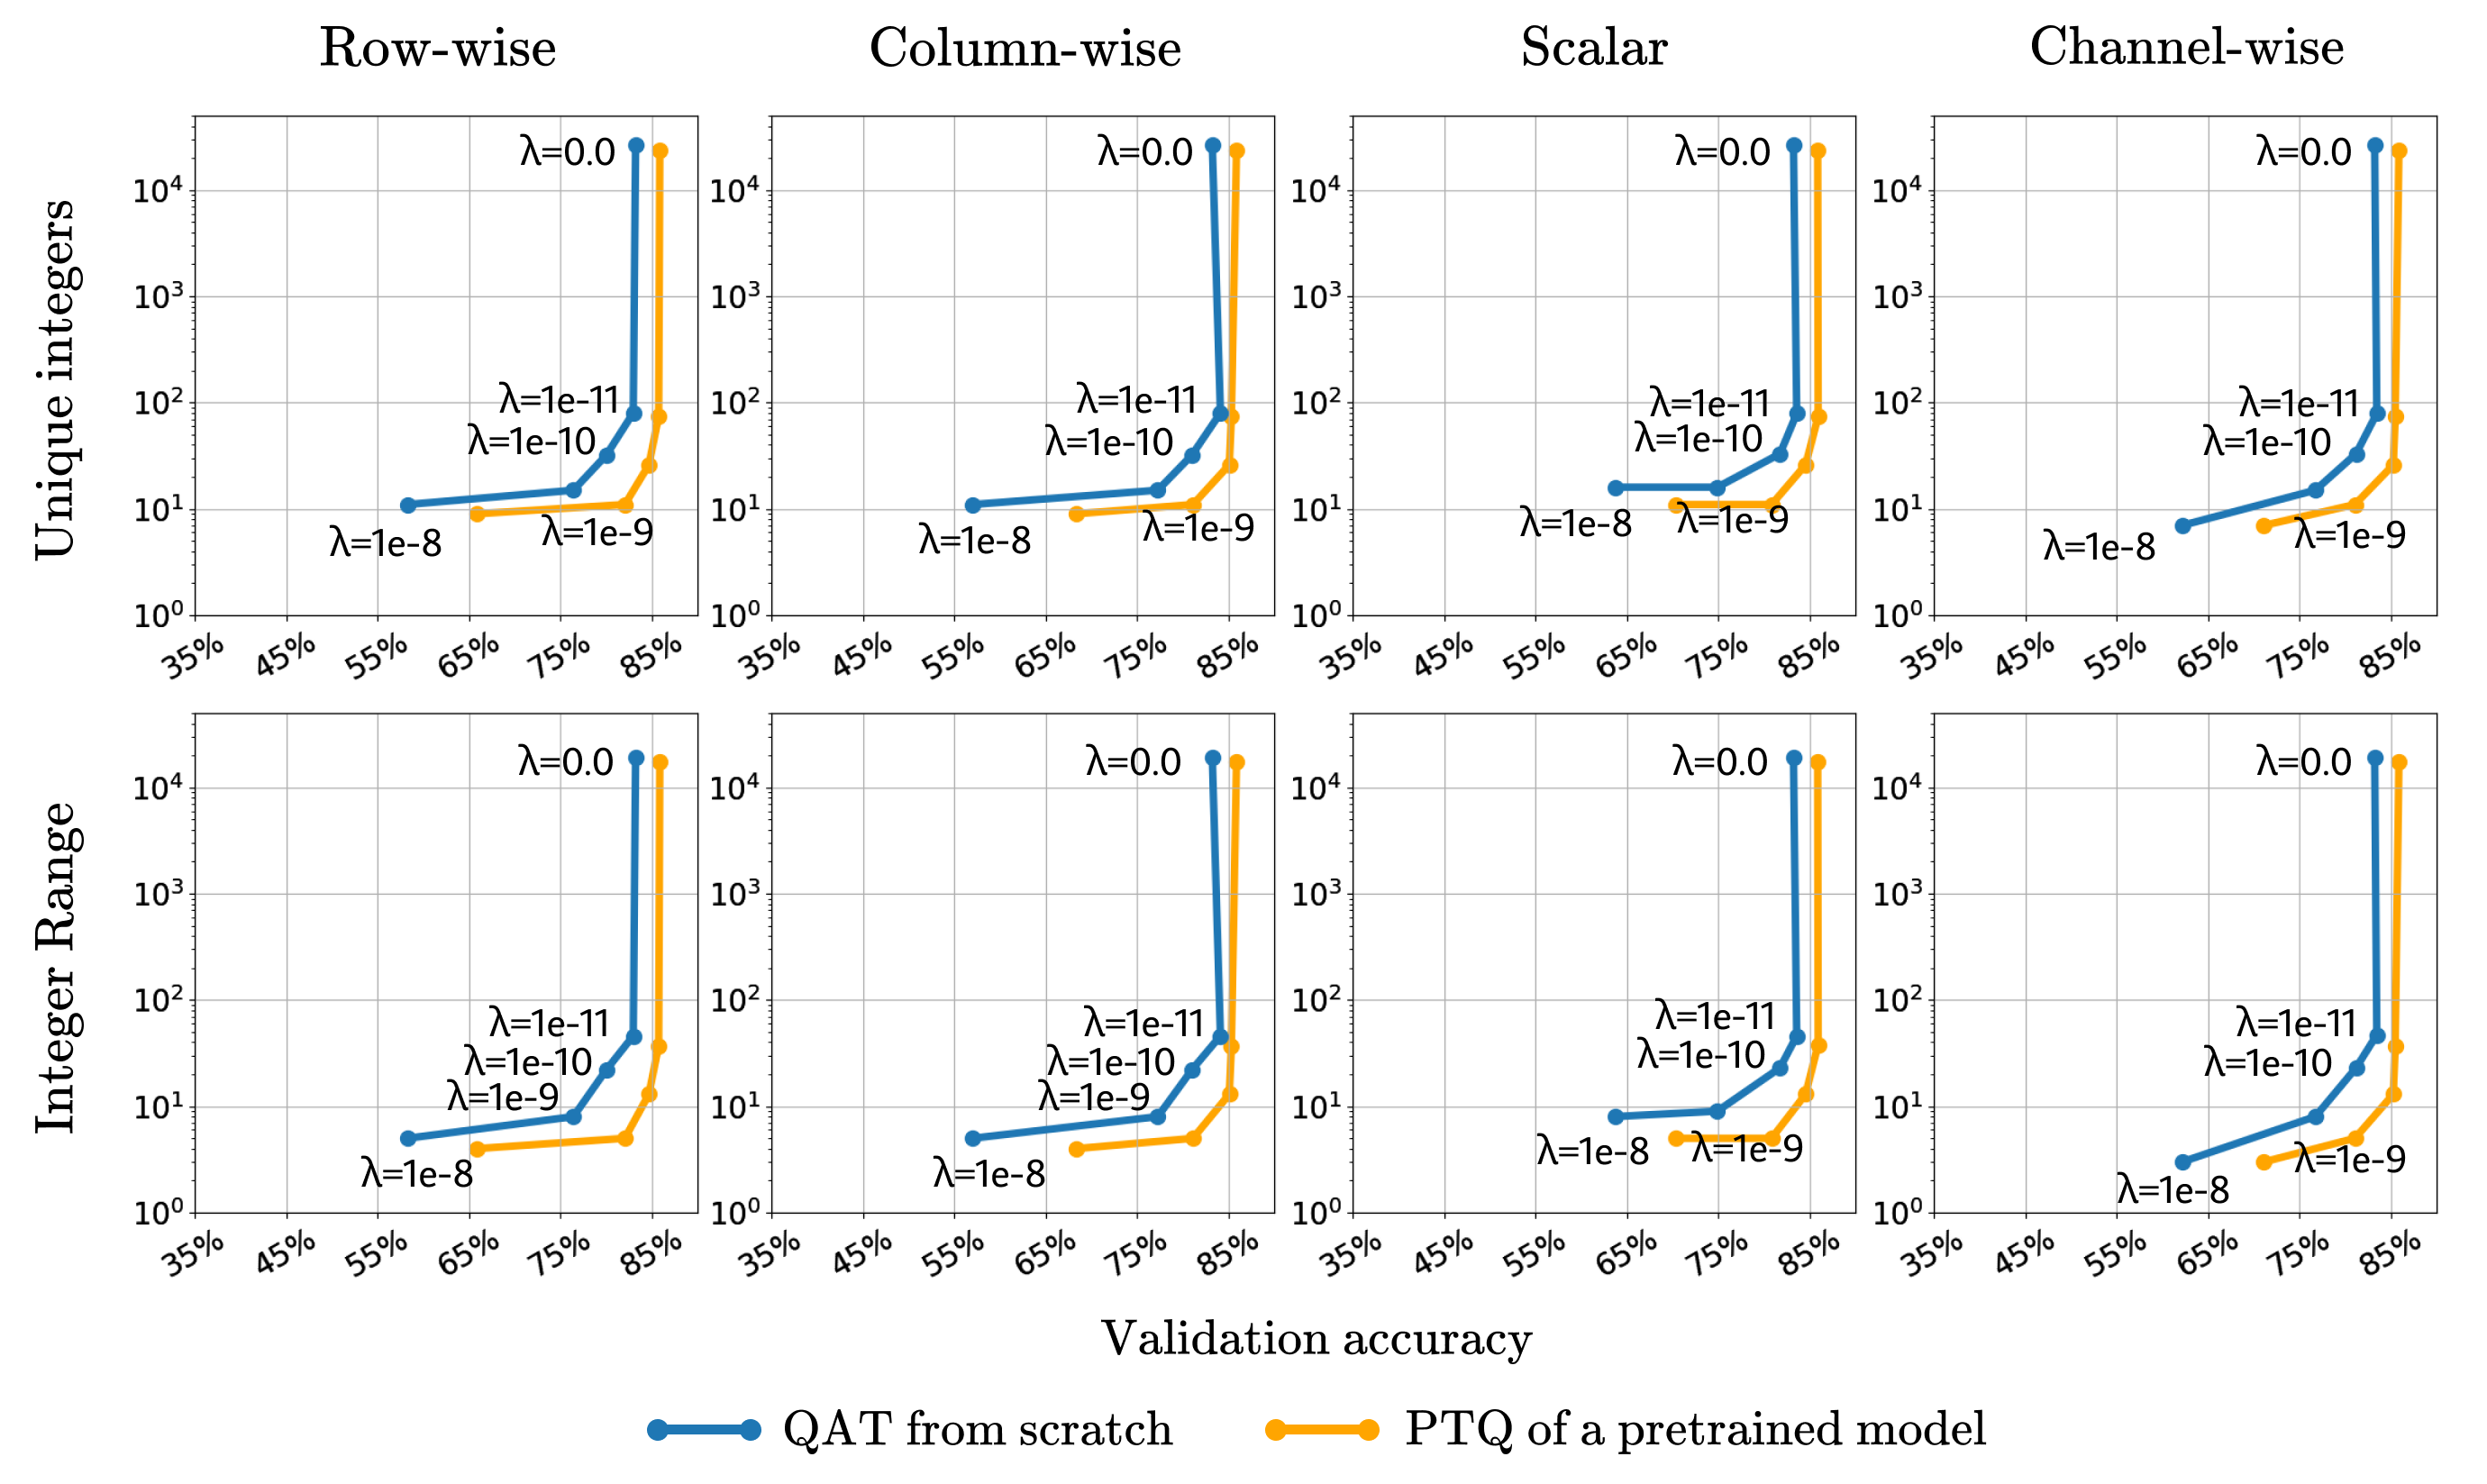
\includegraphics[width=14cm]{Imagenette_nested.png}
  \caption{Accuracy–quantization trade-off for nested quantization layers on Imagenette.}
  \label{fig:imagenette-nested}
\end{figure}


% ------------------------------------------------------------
% ----------------------- Custom loss terms analysis ----------------------- 
% ------------------------------------------------------------
\newpage

\section{Analysis of Custom Loss Terms}
\label{sec:analysisofcustomlossfunctionterms}

\hspace*{1em}For the custom loss term methods, we examine their behavior under different
penalty rates \( \gamma \) for the same three models discussed earlier, 
following a similar approach to the previous section.

% ----------------------- Dense ----------------------- 


\subsection{Fully Connected Layers}
\label{subsec:fullyconnectedlayerscustomloss}

\begin{figure}[t!]
  \centering
  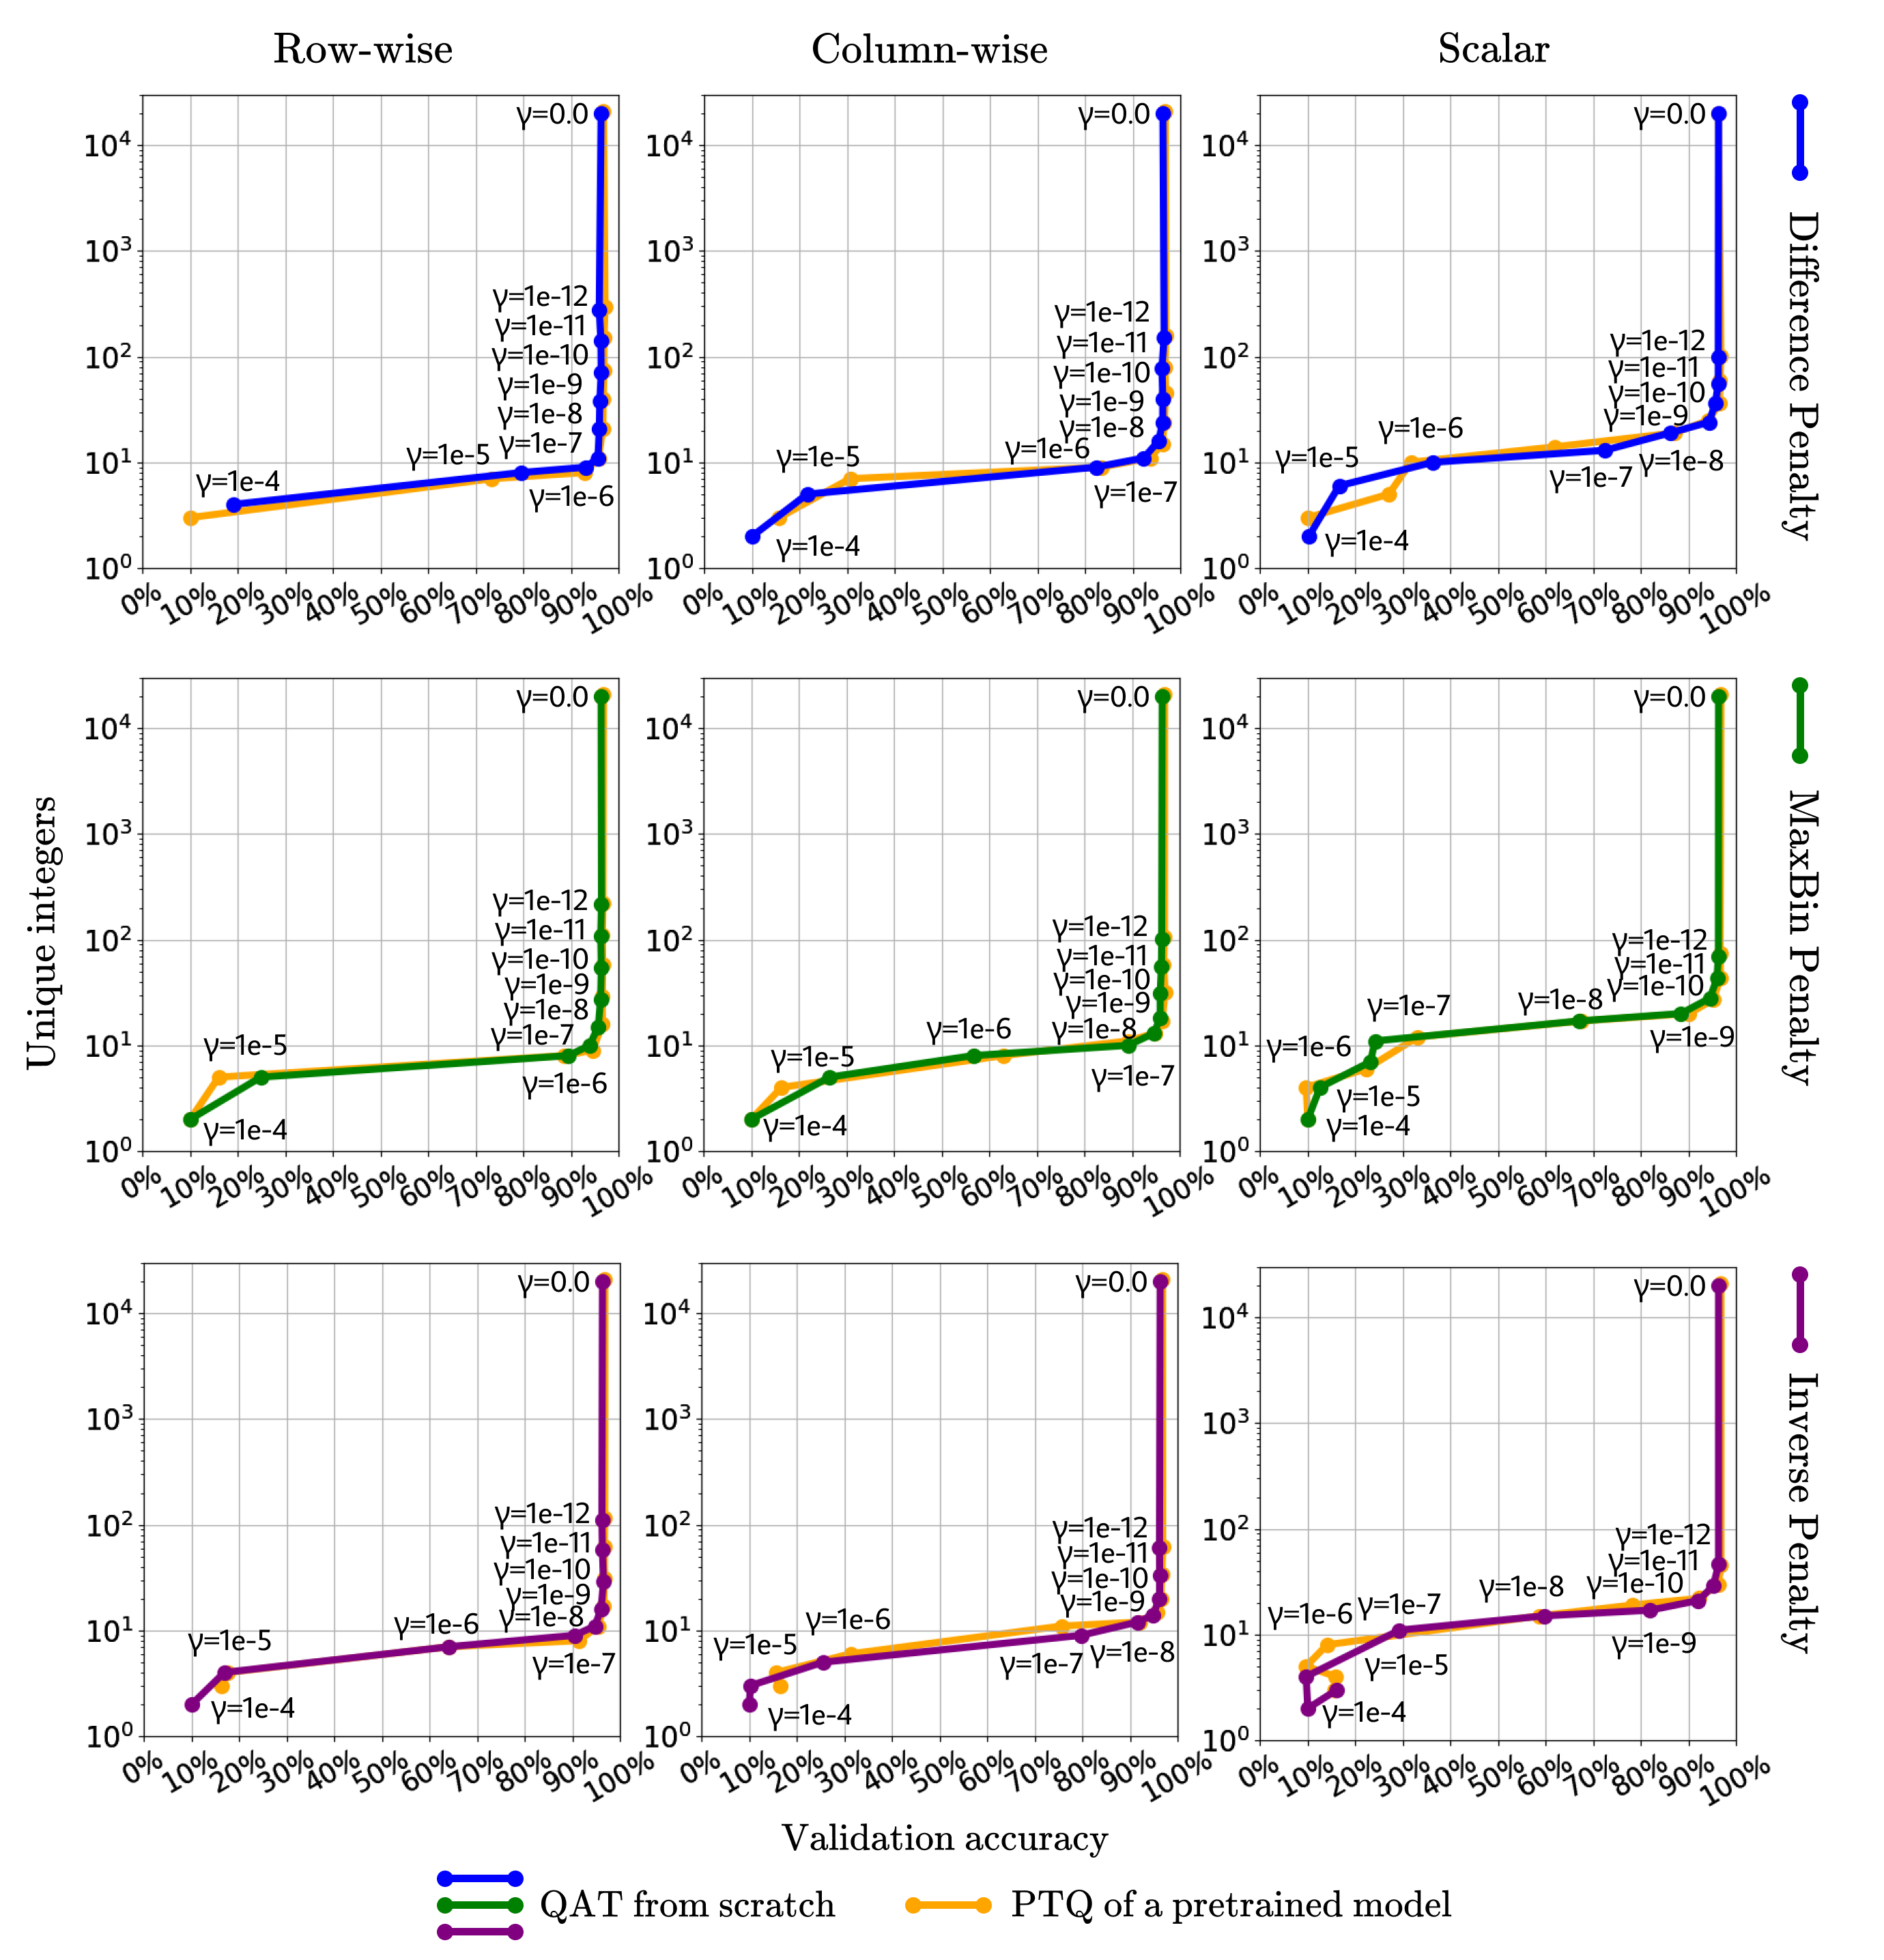
\includegraphics[width=14cm]{mnist_loss.png}
  \caption{Accuracy–quantization trade-off for custom loss terms on MNIST.}
  \label{fig:mnist-loss}
\end{figure}

\hspace*{1em}We compare the three custom loss function terms applied 
to the two dense layers of the model trained on MNIST. 
The resulting Pareto front plots are shown in \cref{fig:mnist-loss}.
We can conclude that the row-wise scenario with the Difference Penalty is the optimal one
as its Pareto front forms the sharpest angle,
the vertex of which is closest to the lower right corner of the plot, indicating an optimal
balance between the number of unique integers and validation accuracy. 
This vertex corresponds to \( \gamma = 1e-7\), that results in integers  
from \(-6 \) to \(2 \),
requiring only \( 4 \) bits, as demonstrated in \cref{fig:quantization_results_1e-7_dense_loss}.

\begin{figure}[t!]
  \centering
  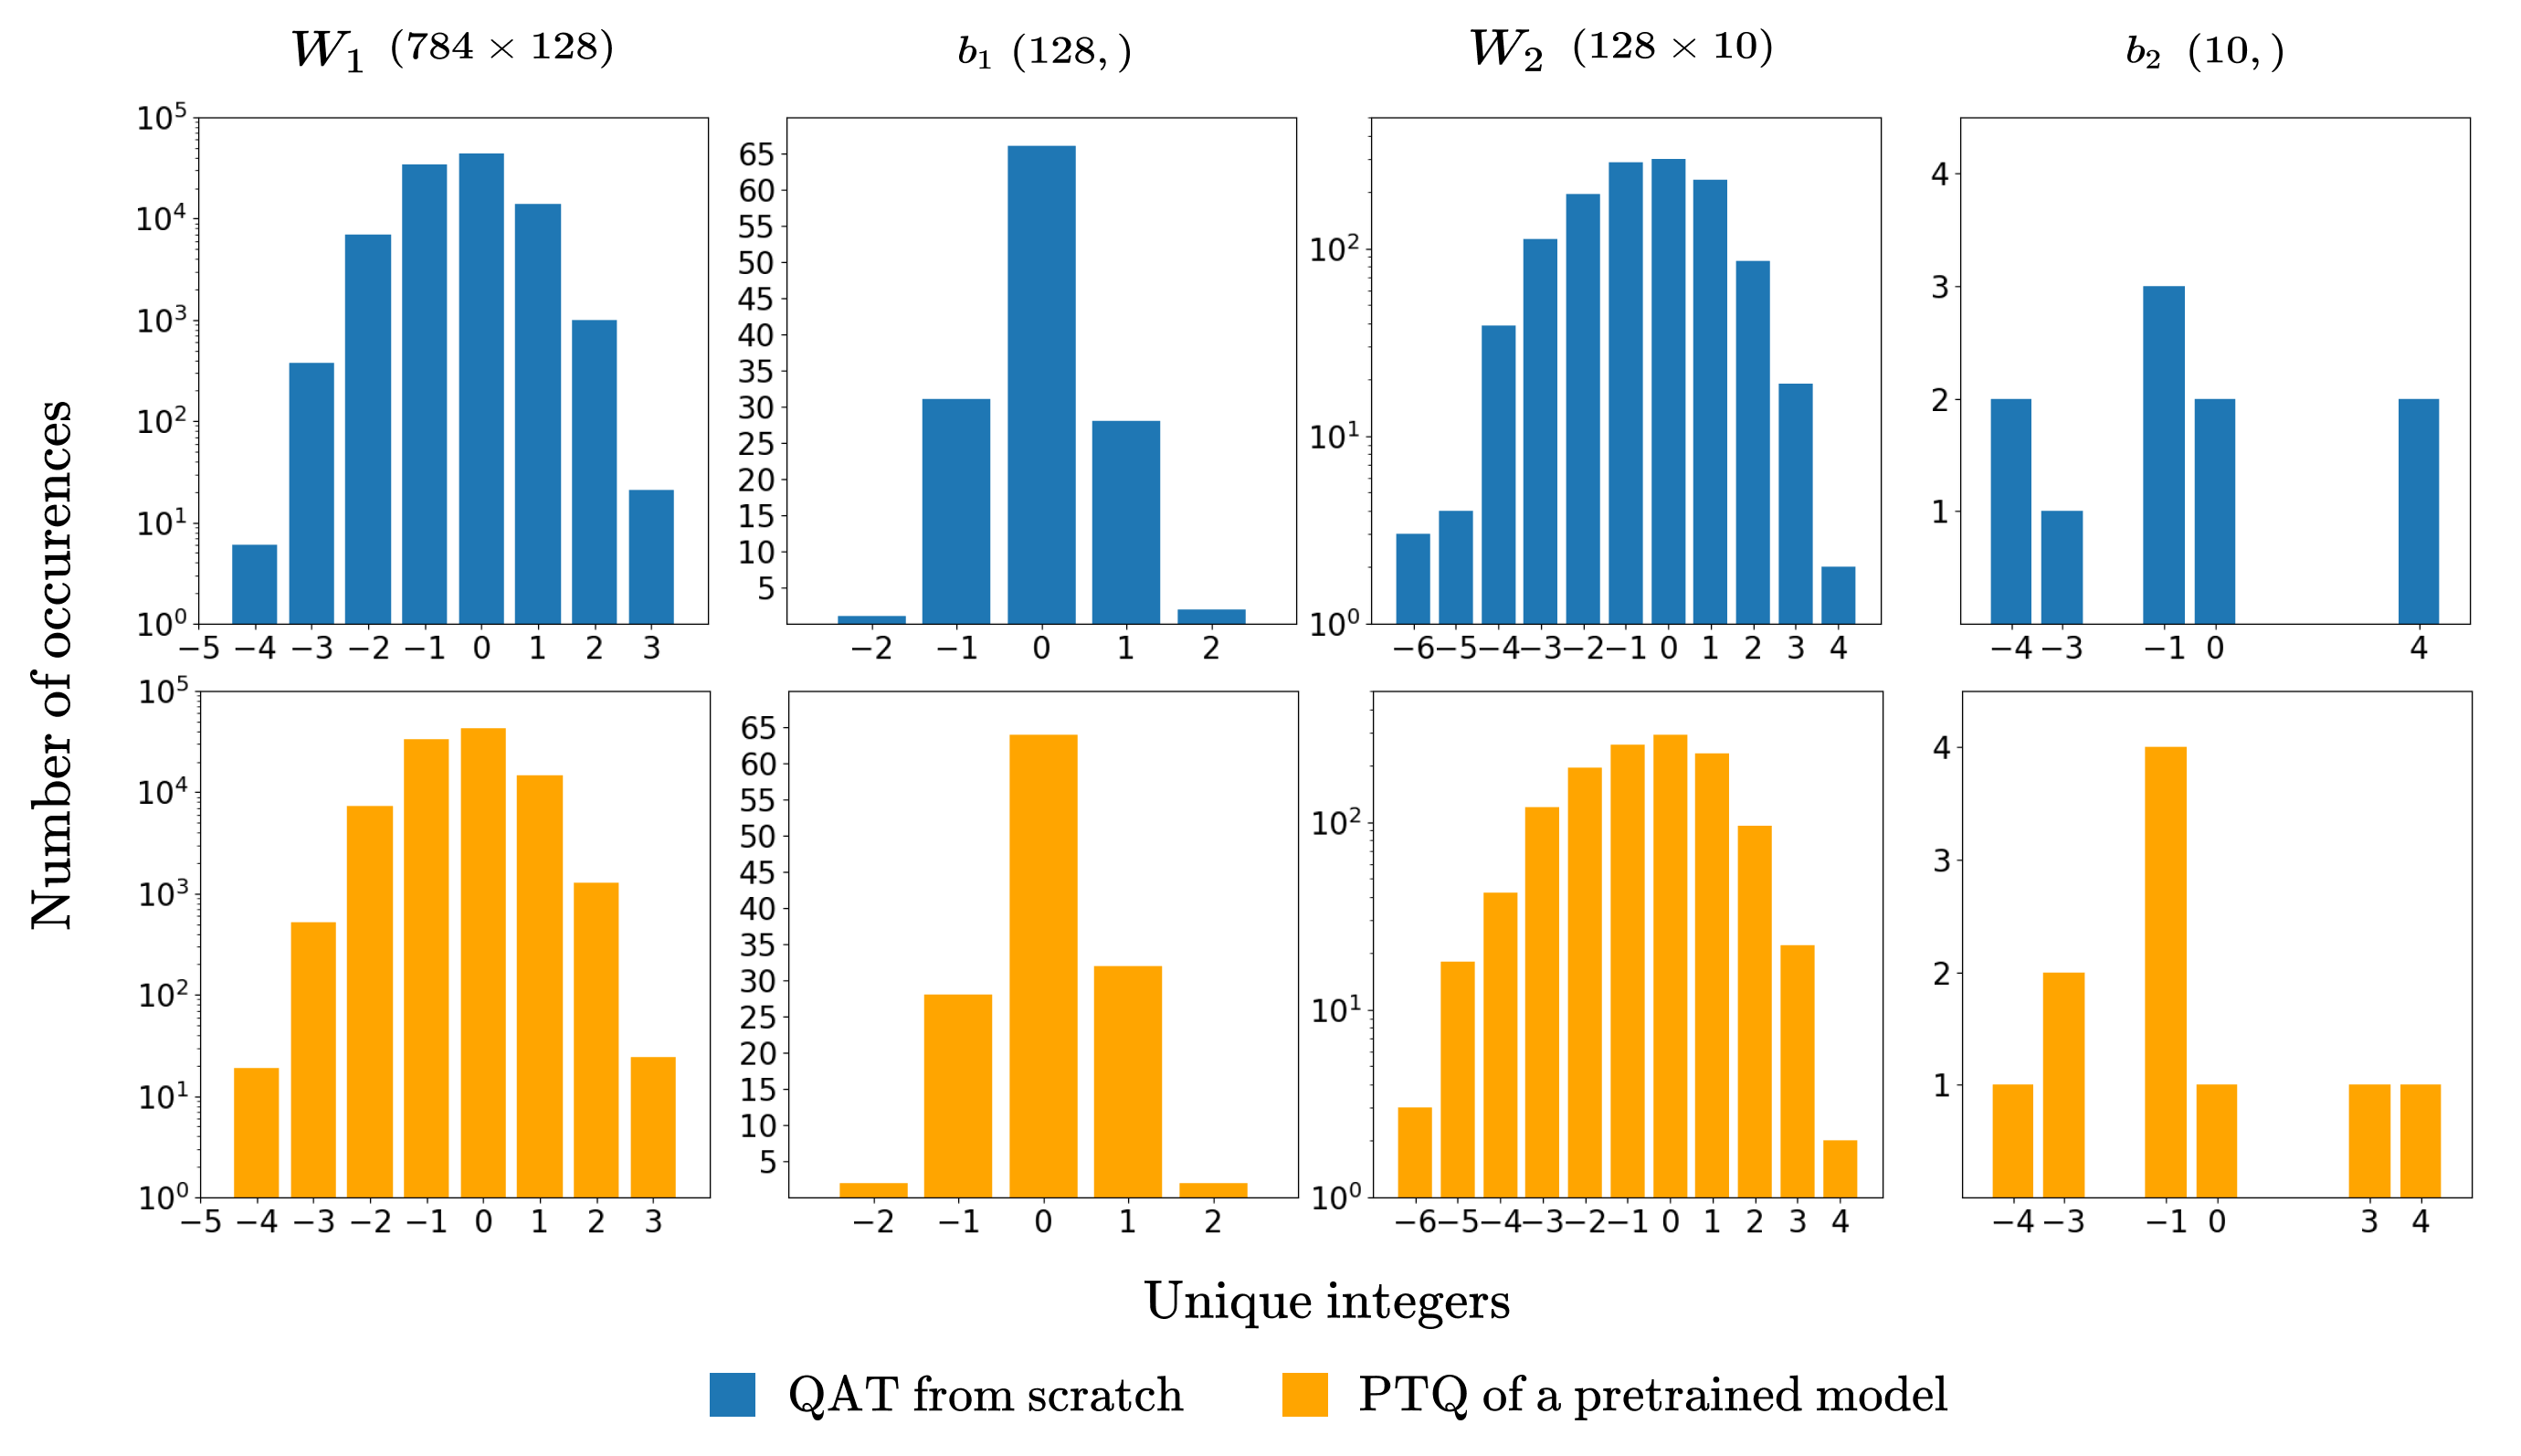
\includegraphics[width=14cm]{quantization_results_1e-7_dense_loss.png}
  \caption{Quantization of MNIST dense layers with row-wise granularity at \( \gamma  = 1e-7 \) with Difference Penalty.}
  \label{fig:quantization_results_1e-7_dense_loss}
\end{figure}

\begin{figure}[t!]
  \centering
  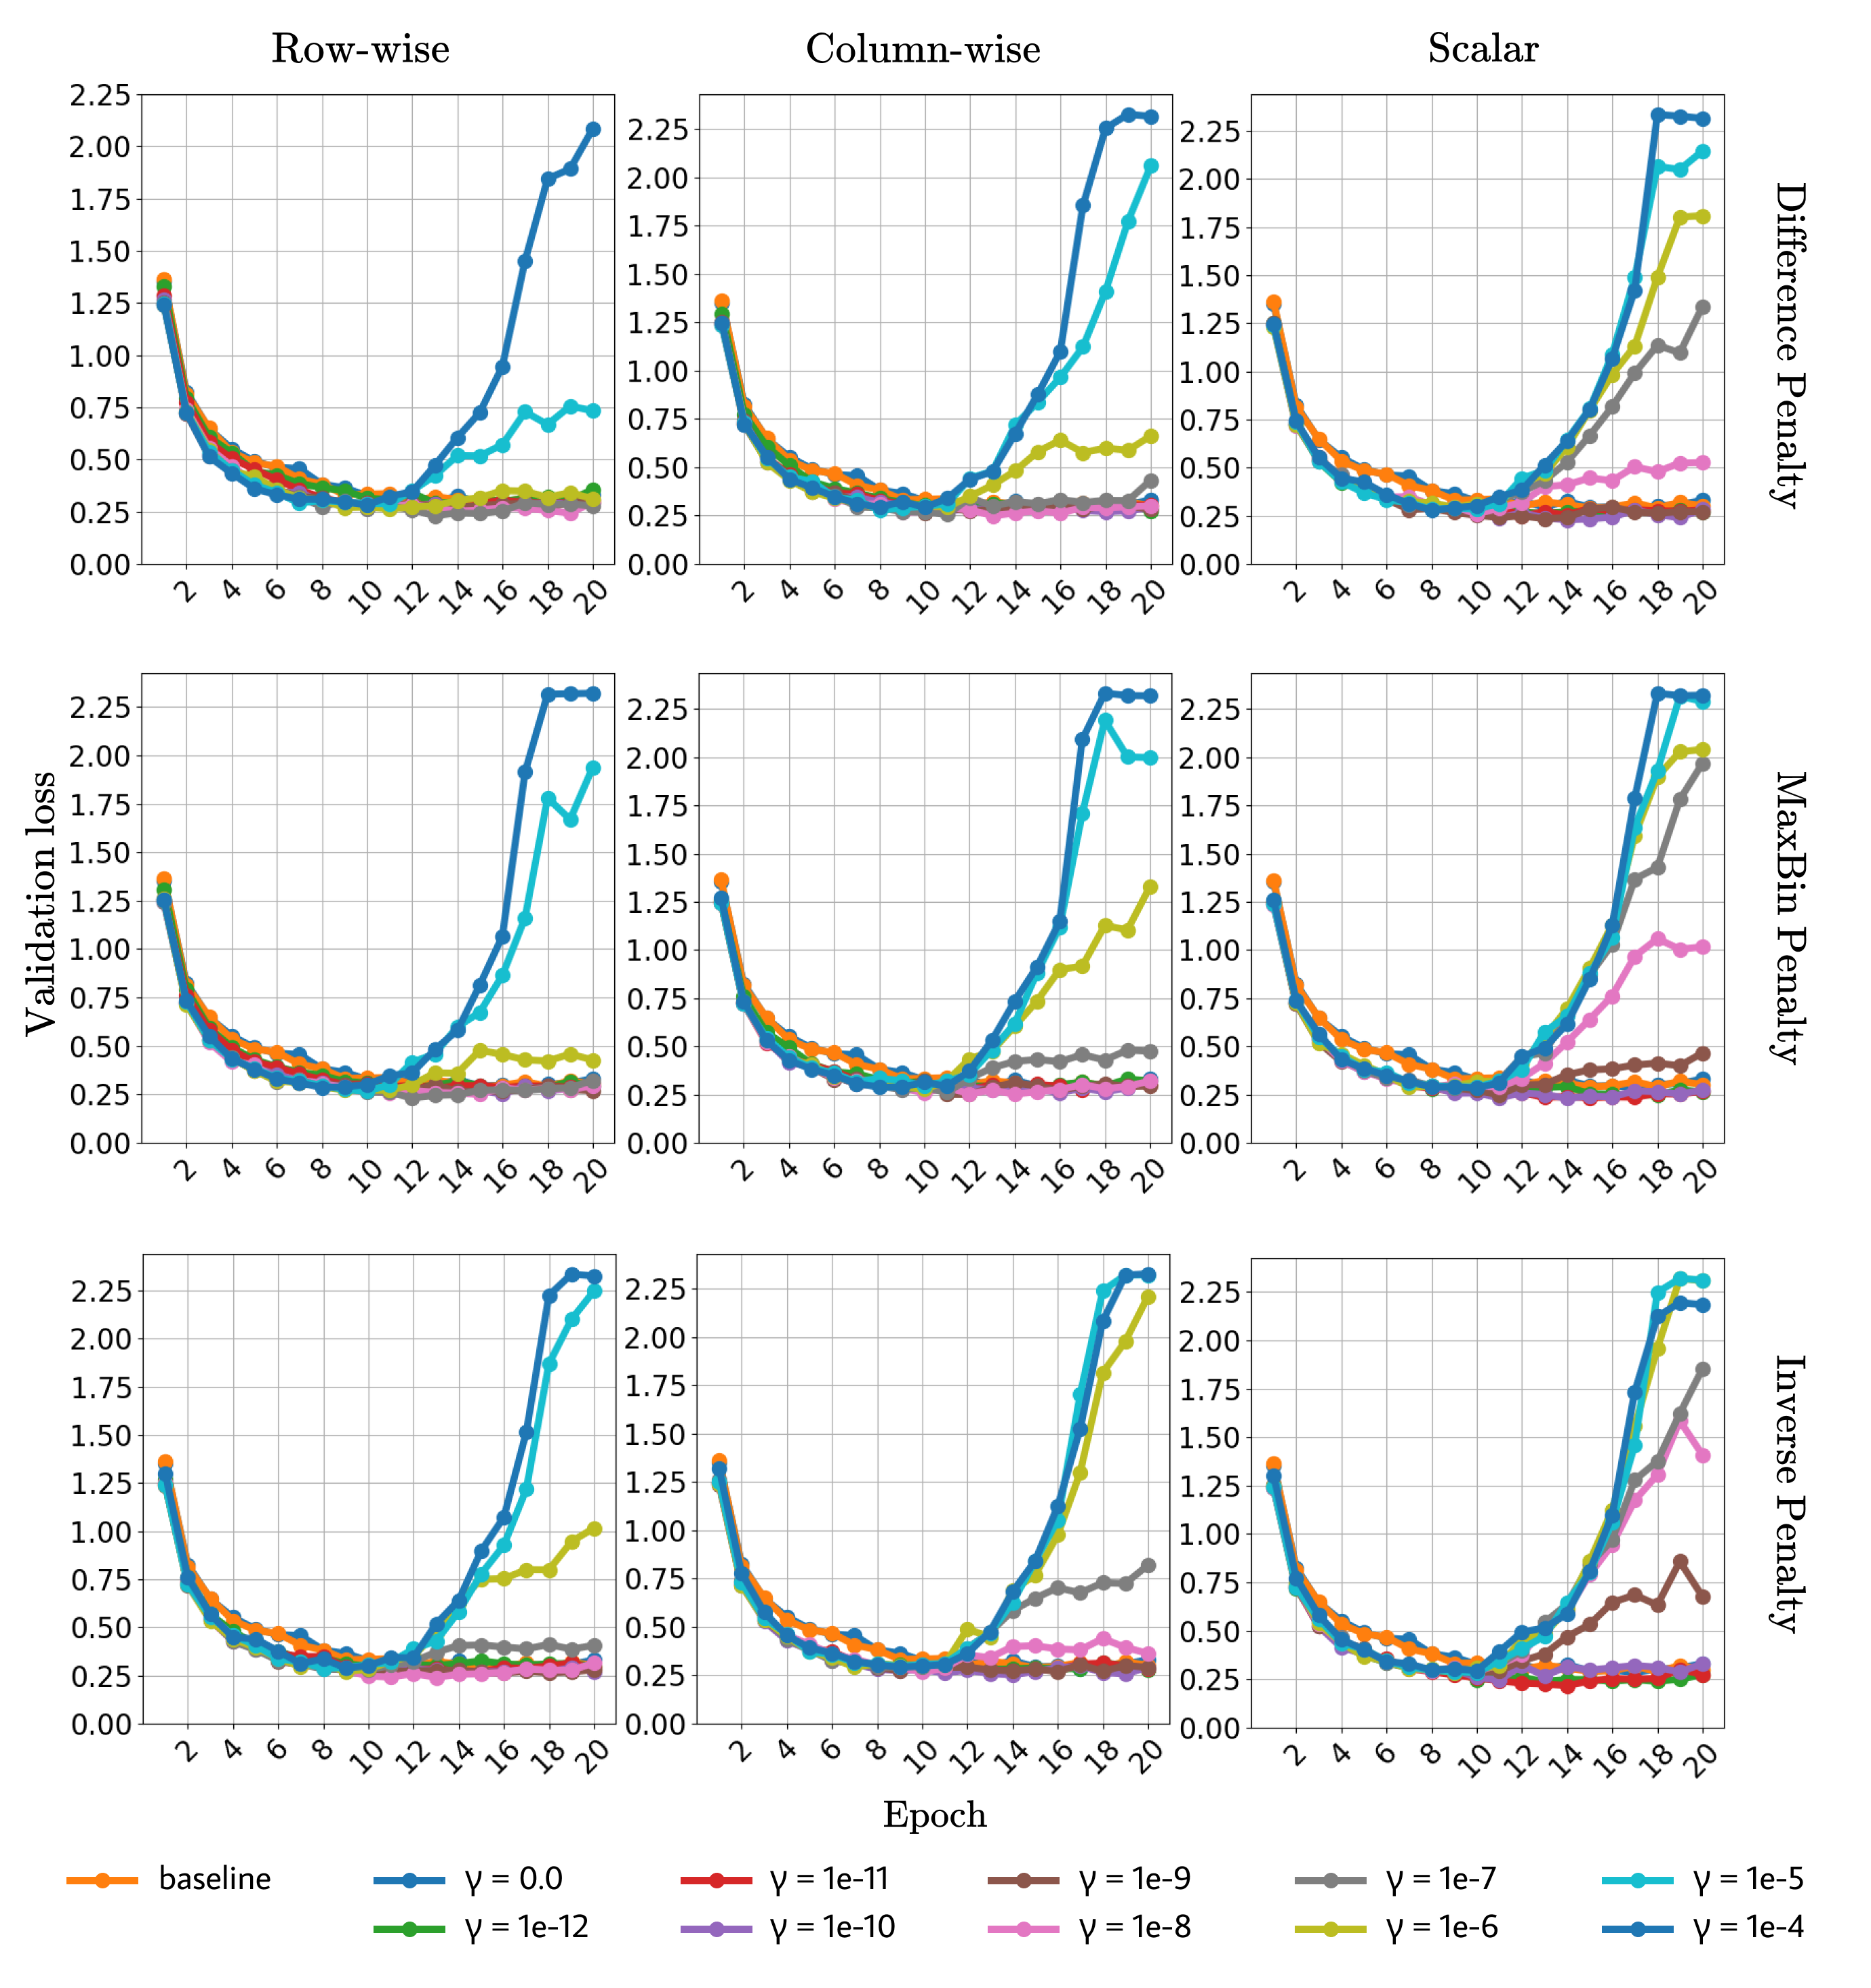
\includegraphics[width=14cm]{mnist-loss-validation.png}
  \caption{Impact of quantization on accuracy and loss for different \( \gamma \) on MNIST.}
  \label{fig:mnist-loss-validation}
\end{figure}

The optimality of the row-wise Difference Penalty case is further supported 
by \cref{fig:mnist-loss-validation}, 
where the validation loss for this scenario starts increasing only at
\( \gamma = 1e-6\), 
while the other granularity and custom loss term combinations
experience a significantly greater increase in loss at the same value of
\( \gamma \). 

From \cref{fig:mnist-loss-validation},we can make the following additional observations.
First, scalar granularity is the most aggressive among the three granularities, 
resulting in the poorest performance due to its excessive coarseness.
Second, the Inverse Penalty stands out as the most aggressive custom loss term,
which is intuitive, as the scale factors are initialized with very small values, 
leading to larger gradient updates proportional to the inverse of these factors.
Consequently, the combination of scalar granularity and the Inverse Penalty performs the worst among all combinations,
although it still achieves reasonably good quantization,
with fewer than 100 unique integers for  \( \gamma = 1e-12 \).


In terms of PTQ, we observe results approximately similar to those of QAT from scratch, 
as shown in \cref{fig:mnist-loss} and \cref{fig:quantization_results_1e-7_dense_loss}. 
The progression of validation loss for each scenario follows the same pattern as in \cref{fig:mnist-loss-validation}, 
although the initial value at the start of training is closer to 0.25 due to the use of a pretrained model.


\newpage

% ----------------------- Conv ----------------------- 

\subsection{Convolutional Layers}
\label{subsec:convolutionallayerscustomloss}

\hspace*{1em} We now compare the loss function terms applied to the convolutional layers of the model trained on CIFAR-10. 
Based on the results summarized in \cref{fig:cifar-loss} and \cref{fig:cifar-loss-validation}, 
the conclusion that the scalar granularity combined with the Inverse Penalty approach is the most aggressive remains valid. 
However, we observe that the channel-wise granularity is the most suitable configuration in this case, 
with \( \gamma = 1e-10 \) producing integers ranging from -28 to 34 in the kernels of the convolutional layers.
These integers form a bell curve closely resembling the experimental results of the nested quantization layer
with rowwise granularity for \( \lambda = 1e-11\) depicted in \cref{fig:quantization-results-1e-10conv}
\begin{figure}[t!]
  \centering
  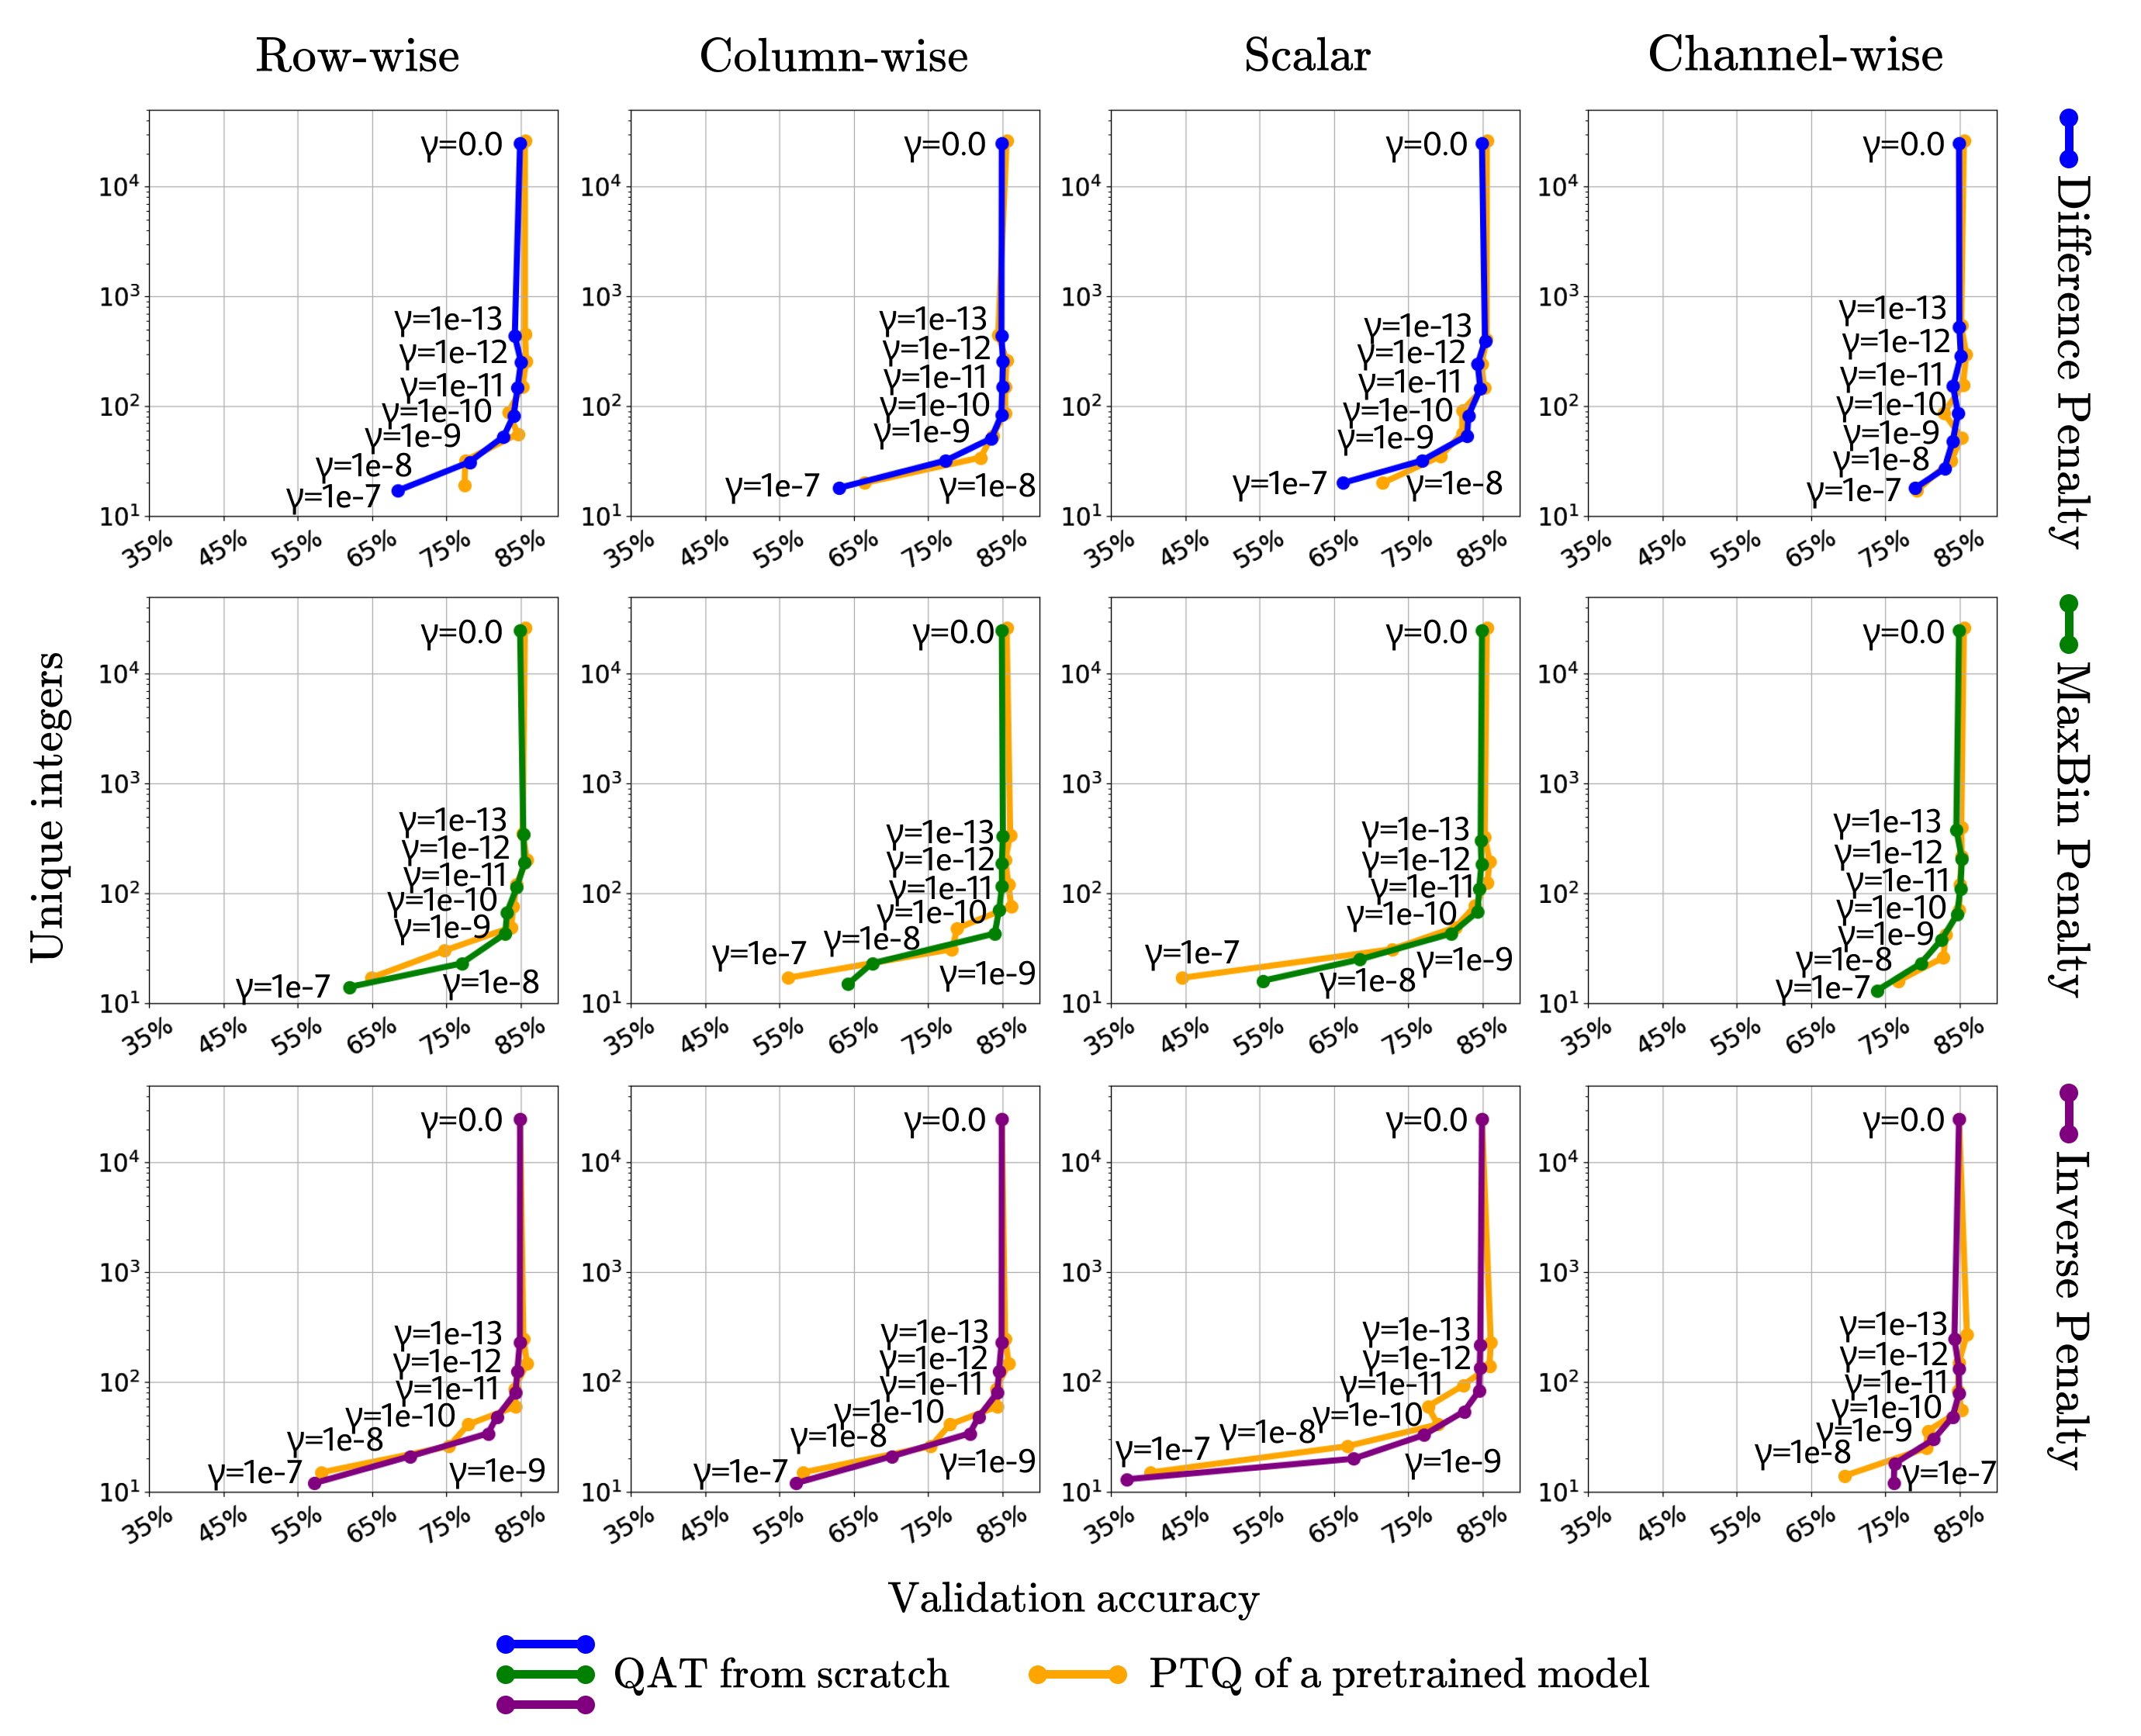
\includegraphics[width=14cm]{cifar_loss.png}
  \caption{Accuracy – Quantization Trade-off for Custom Loss Terms on CIFAR-10.}
  \label{fig:cifar-loss}
\end{figure}
It is worth noting that, 
compared to the gradient-based nested quantization layer approach, the custom loss terms
lead to more outliers in the resulting integers of biases.
This behavior can be attributed to the custom loss term formulations, 
specifically how they are scaled with the number of parameters in each kernel and bias.
Since the bias scale factors affect significantly fewer individual parameters than the kernels, 
their contribution to the loss term is smaller, leading to much smaller updates.

\begin{figure}[t!]
  \centering
  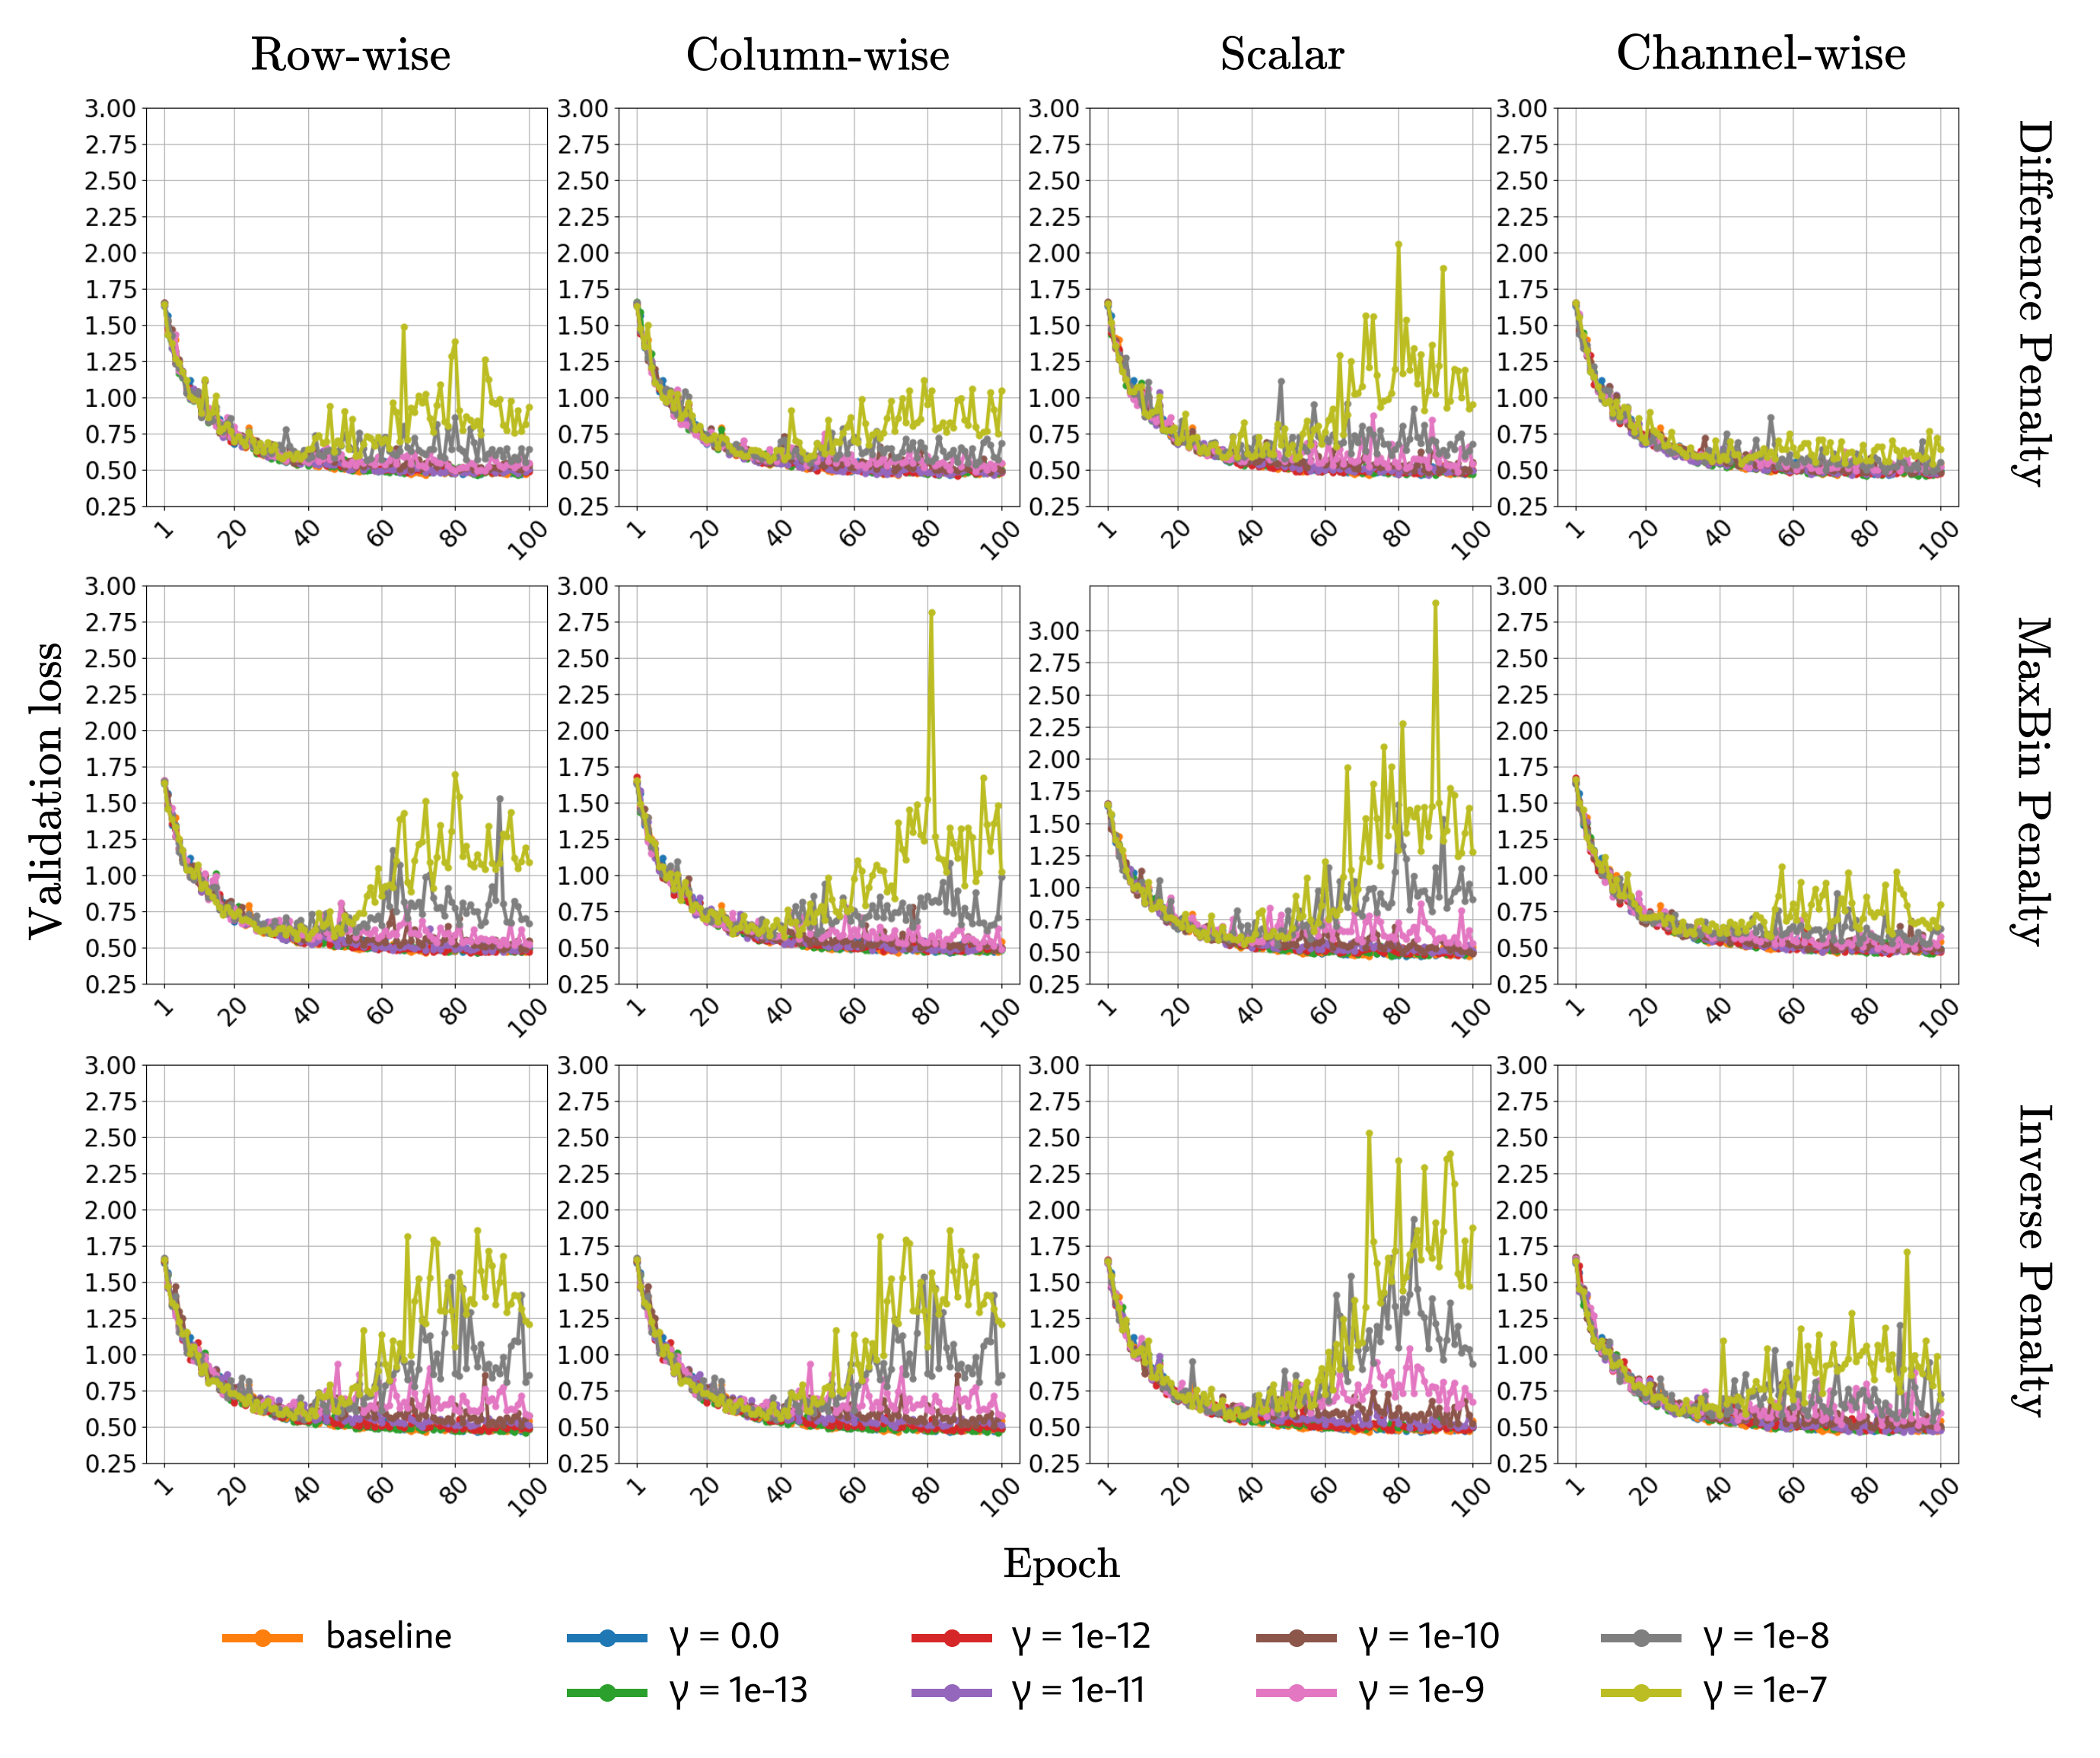
\includegraphics[width=14cm]{cifar-loss-validation.png}
  \caption{Impact of quantization on accuracy and for different \( \gamma \) and custom loss function terms on CIFAR-10.}
  \label{fig:cifar-loss-validation}
\end{figure}

Similar to the other experiments, we conduct PTQ using a full-precision pretrained model. 
The results of PTQ are closely comparable to those obtained through QAT as evident from \cref{fig:cifar-loss}
— which demonstrates the effectiveness of learned quantization in achieving similar outcomes 
without the need for a separate pretraining phase.
Furthermore, the PTQ results for the channel-wise granularity and Difference Penalty combination we highlighted earlier
align closely with those observed in the learned quantization scenario.

\begin{figure}[t!]
  \centering
  \includegraphics[width=14cm]{imagenette_loss.png}
  \caption{Accuracy – Quantization Trade-off for Custom Loss Terms on Imagenette.}
  \label{fig:imagenette-loss}
\end{figure}

For the model trained on Imagenette, 
the custom loss terms fail to form a Pareto front as depicted in \cref{fig:imagenette-loss}, 
although reasonable quantization is achieved with minimal accuracy loss. 
This behavior is attributed to the learning rate decay, 
which prevents the model from reaching a quantization level that could significantly 
impact accuracy once the learning rate becomes too small. In contrast, 
the nested quantization layer approach quantizes more rapidly, ultimately 
"breaking" the model for larger values of the corresponding 
hyperparameter before the learning rate decay limits further updates.

Nevertheless, for the Imagenette dataset, we observe improved accuracy in the PTQ scenario
as noticed in the case with the nested quantization layer. 

Table~\ref{tab:losscomrpessionrate} presents the file sizes of dense or convolutional layers before and after applying our PTQ in selected training scenarios. 
For demonstration purposes, we use the same compression technique as in the nested quantization layer approach.
Across all datasets, we observe a substantial reduction in file size, with reductions sometimes exceeding a factor of 10. 

\begin{table}[t!]
  \centering
  \caption{Compression rate for chosen quantization scenarios}
  \label{tab:losscomrpessionrate}
  \begin{tabular}{lccc}
      \toprule
      \textbf{Combination}     & \textbf{Baseline} & \textbf{PTQ + Compression} & \textbf{Granularity, $\gamma$} \\ 
      \midrule
      MNIST, Difference               & $\approx 0.36 $ MB            & $\approx 0.03 $ MB              & row-wise, $1e-7$         \\ 
      MNIST, MaxBin               & $\approx 0.36 $ MB             & $\approx 0.04 $ MB             &  row-wise, $ 1e-8$           \\ 
      MNIST, Inverse               & $\approx 0.36 $ MB            & $\approx 0.04 $ MB             &  row-wise, $1e-9$          \\ 
      CIFAR-10, Difference          &  $\approx 1.02 $ MB          & $\approx 0.17 $ MB            & channel-wise, $1e-10$            \\ 
      CIFAR-10, MaxBin               &  $\approx 1.02 $ MB            & $\approx 0.15 $ MB              &channel-wise, $ 1e-10$          \\ 
      CIFAR-10, Inverse               &  $\approx 1.02 $ MB            &$\approx 0.16 $ MB              &channel-wise, $1e-11$           \\ 
      Imagenette, Difference               &  $\approx 39.57 $ MB            & $\approx 5.90 $ MB              &channel-wise, $ 1e-9$            \\ 
      Imagenette, MaxBin               &  $\approx 39.57 $ MB        & $\approx 6.46 $ MB             & channel-wise, $1e-9$            \\ 
      Imagenette, Inverse               &  $\approx 39.57 $ MB          & $\approx 5.37 $ MB             & channel-wise, $1e-8$          \\ 

      \bottomrule
  \end{tabular}
  \vspace{1.0em}
\end{table}
    \chapter{Related Work\label{cha:chapter5}}

\hspace*{1em}
\begin{figure}[b!]
    \centering
    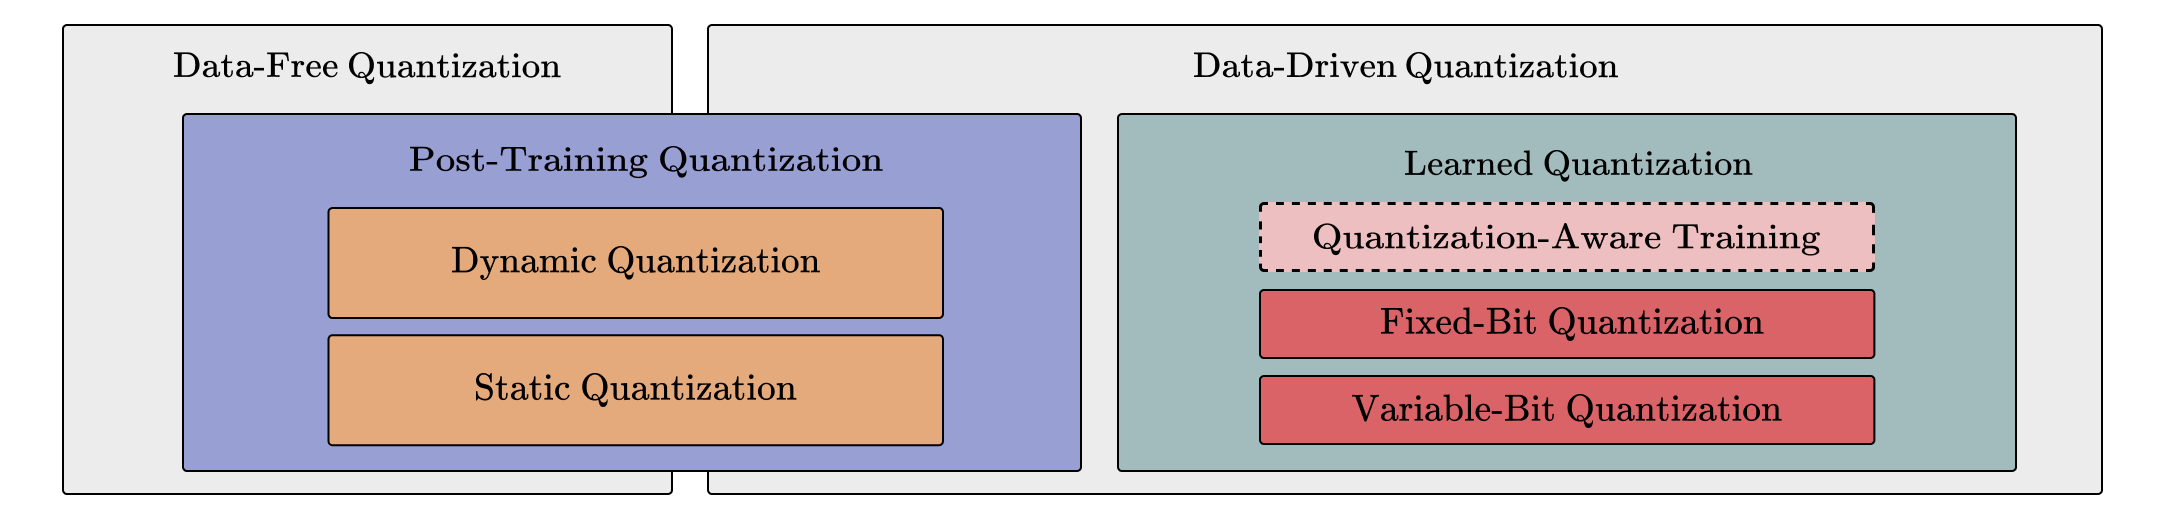
\includegraphics[width=14cm]{related_work.png}
    \caption{ Learned quantization in a broader context.}
    \label{fig:related_work}
  \end{figure}
  
The hyperparameter space of deep neural networks is so vast
that classifying research in the field of learned quantization into rigid groups
is inherently challenging.
Nevertheless, we aim to outline a rough distinction
between different approaches by emphasizing their most apparent aspects,
after first establishing the position of learned quantization within the broader field of quantization.

\textbf{Data-Free vs. Data-Driven Quantization.}
As discussed in \cref{cha:chapter2}, 
data-free quantization relies solely on the intrinsic properties of ML models, 
such as weight distribution statistics, to determine quantization parameters \cite{DBLP:conf/iccv/NagelBBW19}. 
In contrast, data-driven quantization uses the original training data to fine-tune the model to the quantization strategy \cite{Edouard2022SPIQ}. 
Although learned quantization does not strictly align with the definition of a fine-tuning process, 
it incorporates the full training pipeline, jointly optimizing both the model and the quantization parameters. 
This characteristic makes it inherently data-driven. 
Thus, we regard learned quantization as a distinct subcategory within data-driven quantization approaches.

\textbf{PTQ vs. QAT.}
PTQ \cite{DBLP:conf/icmcs/ZhuZL18} can fall into either the data-free or data-driven category, depending on the parameters being quantized. 
If it’s just weights, it’s data-free since weights can be quantized without relying on input data. 
However, if activations are included, it’s data-driven because activation quantization needs input data for calibration. 
Since PTQ doesn’t involve training on the full dataset, it’s distinct from learned quantization.
QAT, on the other hand, does involve full training, where the model adapts to the quantization strategy. 
This makes it part of learned quantization, which may also involve learning the quantization parameters themselves as part of the process.

\textbf{Static vs. Dynamic Quantization.} 
Static quantization is an offline method that quantizes weights and activations before inference, 
whereas dynamic quantization is applied on-the-fly during inference. 
Both static and dynamic quantization methods are post-training approaches. 
In the context of learned quantization, 
static quantization might refer to a fixed quantization scheme, 
and dynamic quantization  — to a scheme 
that depends on trainable quantizers.
However, these terms are not commonly used this way in the literature.
Therefore, we consider static and dynamic quantization separately from learned quantization. 

Having established the broader context of quantization, 
we will now attempt to classify the various approaches within learned quantization itself.

\textbf{Fixed-Bit vs. Variable-Bit.} 
Learned quantization schemes can be roughly divided into two broader groups. 
The first group involves quantization schemes that use a fixed target bit size, 
while the second group aims to learn or effectively determine the lowest feasible bit size. 
This distinction is not widely discussed in the literature, 
but we view it as a recognizable pattern. 
For example, LQ-Nets \cite{DBLP:conf/eccv/ZhangYYH18} compute binary encodings of model parameters using a predefined bit size, 
whereas LSQ \cite{DBLP:conf/iclr/EsserMBAM20} learns step sizes in a way that can adaptively reduce bit width requirements.

\textbf{Quantization Target.} NNs offer multiple opportunities for applying quantization.
While some learned quantization approaches focus exclusively on model weights \cite{polino2018modelcompression} \cite{ott2016rnn} \cite{courbariaux2015binaryconnect} \cite{DBLP:journals/pnas/EsserMACAABMMBN16},
others extend this to include activations \cite{krishnamoorthi2018quantizing} \cite{hubara2016qnn} \cite{rastegari2016xnor} \cite{Edouard2022SPIQ} \cite{DBLP:conf/eccv/ZhangYYH18}
and even gradients \cite{DBLP:journals/corr/LinCMB15} \cite{DBLP:conf/icml/Zhang0KALZ17}. As notable examples,
DoReFa-Net \cite{shuchang2016dorafenet} quantizes all three with arbitraty bitwidths, 
whereas Quantized Neural Networks \cite{hubara2016qnn} constrain weights and activations to either 
\( -1 \) or \( +1 \), and quantize gradients to \( 6 \) bits.

\textbf{Quantization Precision.}
The target lower bit precision, and whether it is adjustable, 
varies between methods — ranging from rigid constraints to only a few values, 
to the flexibility of setting the desired bitwidth. 
For instance, BinaryNet \cite{DBLP:conf/nips/HubaraCSEB16} and XNOR-Net \cite{rastegari2016xnor} 
represent extreme cases of quantization, 
where weights and activations are binarized. 
Ternary Weight Networks \cite{DBLP:conf/icassp/LiuLWZY23} take a slightly less aggressive approach 
by quantizing weights to \( -1, 0, 1 \). 
In contrast, DoReFa-Net \cite{shuchang2016dorafenet} allows the target bit size to be defined.

\textbf{Quantization Granularity.} 
Learned quantization methods differ in how granularly the quantization is applied, 
that is, the level of detail at which model parameters are quantized. 
To illustrate, Benoit et al. \cite{jacob2018quantization} implement layer-wise quantization  — 
similar to QIL \cite{DBLP:conf/cvpr/JungSLSHKHC19} and PACT \cite{DBLP:journals/corr/abs-1805-06085}  — 
whereas LQ-Nets \cite{DBLP:conf/eccv/ZhangYYH18} employ channel-wise quantization for weights, 
despite using layer-wise quantization for activations.

\textbf{Combination with Other Techniques.} 
A number of learned quantization methods work in unison with other model compression approaches.
For example, Deep Compression \cite{han2016deepcompression} combines quantization with pruning, while 
Polino et al. \cite{polino2018modelcompression} and Wei et al. \cite{DBLP:conf/eccv/WeiPQOY18} 
jointly leverage quantization and knowledge distillation.

To summarize, the landscape of learned quantization is as diverse as it gets.
While the classifications outlined in this chapter are by no means exhaustive, 
they represent those we find most apparent and distinguishable.
Together with \cref{cha:chapter2}, 
this chapter aims to provide a broader pitcture of learned quantization. 
Building on this picture,
we will reflect on the contributions of this thesis and outline potential directions for future research in the conclusion.

    \chapter{Conclusions\label{cha:chapter6}}

Bullet points:
- not all layers react similarly to quantization. This gives room for experimenting with
different thresholds for different Layers
- combined scenarios are not tested 
- could be tested on standard networks like ALexNet
- The scale updates will potentially be improved by some kind of normalization/heuristics
- Most literature argues that having an additional parameter to tune is based
- The grad calculation may be considered a bit too much
- In real life, if the model is hard to track, it will be hard to finetune

- but this is, if not the first, then at least one of the first 
approaches that is based on the gradient of the parameter
- there's also a theory that the ratio |dy| / |paramter| converges for all parameters,
so this is very valid
- the nested logic is cool

% ---------------------------------------------------------------
\backmatter % no page numbering from here
    %\addchap{List of Acronyms}

\begin{tabbing}
spacespacespace \= space \kill
ML	 \> 	Machine Learning	 \\
\end{tabbing}
\endinput

		
		% if you want to provide a glossary with explanations of important terms put it in here

    % \bibliographystyle{geralpha}
    % \bibliography{./bib/manual}
    \printbibliography  
    % \addchap{Appendix}

\begin{appendix}

Add additional experimental results that do not need to be directly included in the thesis body. 

\end{appendix}

\endinput


\end{document}
